% =====================================================================
%  main.tex —— 汇总文件（Lead 独占）
%  植田一石《ホモロジー的ミラー対称性》中文译注本
%  编译：xelatex main.tex（连续两遍）
% =====================================================================
% =====================================================================
%  preamble.tex —— 导言区（Lead 独占；译者只读，不得修改）
%  植田一石《ホモロジー的ミラー対称性》（东京大学 2015 年度冬学期讲义录）
%  中文译注本 · XeLaTeX 编译
% =====================================================================
\documentclass[11pt,a4paper]{article}

\usepackage[UTF8]{ctex}
\usepackage{amsmath,amssymb,amsthm,mathtools}
\usepackage{bm}
\usepackage{graphicx}
\usepackage[a4paper,left=2.4cm,right=2.4cm,top=2.6cm,bottom=2.7cm]{geometry}
\usepackage[dvipsnames]{xcolor}
\usepackage{enumitem}
\usepackage{booktabs}
\usepackage{array}
\usepackage{multicol}
\usepackage{fancyhdr}
\usepackage{caption}
\usepackage{titlesec}
\usepackage[hidelinks,unicode]{hyperref}
\hypersetup{pdftitle={同调镜像对称（中文译注本）},
  pdfauthor={植田一石 著；中文译注：本工程}}

\captionsetup{font=small,labelsep=quad}
\setlength{\emergencystretch}{3em}
\allowdisplaybreaks[1]
\graphicspath{{figures/}{../work/figures/}{work/figures/}}

% ---------- 节标题：原文「第 N 節」 ----------
\titleformat{\section}{\Large\bfseries}{第 \thesection{} 节}{1em}{}
\titlespacing*{\section}{0pt}{22pt}{12pt}
\titleformat{\subsection}{\large\bfseries}{\thesubsection}{1em}{}
\titleformat{\subsubsection}[runin]{\bfseries}{\thesubsubsection.}{0.5em}{}

% ---------- 页眉页脚 ----------
\pagestyle{fancy}
\fancyhf{}
\fancyhead[L]{\small\itshape Homological Mirror Symmetry}
\fancyhead[R]{\small 同调镜像对称\quad\thepage}
\renewcommand{\headrulewidth}{0.4pt}

% ---------- 定理类环境：全节共享一个计数器 ----------
% 原文：定義 30.1 / 定理 30.3 / 命題 30.4 …（同一节内连续编号）
\theoremstyle{plain}
\newtheorem{theorem}{定理}[section]
\newtheorem{definition}[theorem]{定义}
\newtheorem{proposition}[theorem]{命题}
\newtheorem{lemma}[theorem]{引理}
\newtheorem{corollary}[theorem]{推论}
\newtheorem{example}[theorem]{例}
\newtheorem{claim}[theorem]{断言}
\newtheorem{conjecture}[theorem]{猜想}
\newtheorem{question}[theorem]{问题}
\newtheorem{exercise}[theorem]{习题}
\theoremstyle{definition}
\newtheorem{remark}[theorem]{注}
\newtheorem{notation}[theorem]{记号}
\newtheorem{construction}[theorem]{构造}

% ---------- 常用宏 ----------
\newcommand{\R}{\mathbb{R}}
\newcommand{\C}{\mathbb{C}}
\newcommand{\Z}{\mathbb{Z}}
\newcommand{\N}{\mathbb{N}}
\newcommand{\Q}{\mathbb{Q}}
\newcommand{\PP}{\mathbb{P}}
\newcommand{\kk}{k}
\newcommand{\dd}{\mathrm{d}}
\newcommand{\ee}{\mathrm{e}}
\newcommand{\ii}{\mathrm{i}}
\newcommand{\id}{\mathrm{id}}
\newcommand{\rank}{\operatorname{rank}}
\newcommand{\Hom}{\operatorname{Hom}}
\newcommand{\End}{\operatorname{End}}
\newcommand{\Ext}{\operatorname{Ext}}
\newcommand{\Tot}{\operatorname{Tot}}
\newcommand{\Spec}{\operatorname{Spec}}
\newcommand{\Coh}{\operatorname{Coh}}
\newcommand{\Perf}{\operatorname{Perf}}
\newcommand{\Dcoh}{D^{b}(\Coh)}
\newcommand{\Fuk}{\mathcal{F}}
\newcommand{\cA}{\mathcal{A}}\newcommand{\cB}{\mathcal{B}}\newcommand{\cC}{\mathcal{C}}
\newcommand{\cD}{\mathcal{D}}\newcommand{\cE}{\mathcal{E}}\newcommand{\cF}{\mathcal{F}}
\newcommand{\cG}{\mathcal{G}}\newcommand{\cH}{\mathcal{H}}\newcommand{\cI}{\mathcal{I}}
\newcommand{\cL}{\mathcal{L}}\newcommand{\cM}{\mathcal{M}}\newcommand{\cN}{\mathcal{N}}
\newcommand{\cO}{\mathcal{O}}\newcommand{\cP}{\mathcal{P}}\newcommand{\cS}{\mathcal{S}}
\newcommand{\cT}{\mathcal{T}}\newcommand{\cU}{\mathcal{U}}\newcommand{\cV}{\mathcal{V}}
\newcommand{\cW}{\mathcal{W}}\newcommand{\cX}{\mathcal{X}}\newcommand{\cY}{\mathcal{Y}}
\newcommand{\cZ}{\mathcal{Z}}
\newcommand{\fg}{\mathfrak{g}}\newcommand{\fM}{\mathfrak{M}}\newcommand{\fT}{\mathfrak{T}}
\newcommand{\fX}{\mathfrak{X}}\newcommand{\fY}{\mathfrak{Y}}\newcommand{\fZ}{\mathfrak{Z}}

% 原文行内粗体小标题（如「**定義.**」）用这个
\newcommand{\para}[1]{\par\noindent\textbf{#1}\quad}

% 图注：原文「図 13.1: ...」→ 印「图 13.1：...」
\newcommand{\figtitle}[2]{\caption*{图 #1：\ #2}}
% 表注
\newcommand{\tabtitle}[2]{\caption*{表 #1：\ #2}}

% 译者注框（审校批注就地引用时用；正文不滥用）
\newcommand{\transnote}[1]{\par\smallskip\noindent{\small\color{Sepia}【译者注】#1}\smallskip\par}

\setlength{\parindent}{2em}
\setcounter{tocdepth}{2}


\title{\bfseries 同调镜像对称\\[6pt]
  \large\mdseries 植田一石 著 · 中文译注本}
\author{原作：植田一石（大阪大学／东京大学）\\[2pt]
  \small 底本：东京大学大学院数理科学研究科 2015 年度冬学期讲义录}
\date{2026 年}

\begin{document}
\maketitle
\thispagestyle{empty}

\vspace{2em}
\begin{center}
\begin{minipage}{0.86\textwidth}
\small
\textbf{译本说明}\quad
本译本依据植田一石教授 2015 年度冬学期于东京大学大学院数理科学研究科讲授的
「同调镜像对称」讲义录（PDF 64 页）译出。原文按「節」编号（共 34 节），
译本保留原编号与节标题的语义，公式编号（如 (2.1)、(30.3)）与原文一一对应。
翻译中公式一律以原页面图像为准逐符号核对；原文的省略、含糊或疑似笔误，
一律不补写、不改写，只在批注中标出。
\end{minipage}
\end{center}

\vspace{1em}
\tableofcontents
\newpage

% =====================================================================
% c00.tex —— 第 1 节「はじめに」/ 第 2 节「ミラー対称性」（p001–p005）
% 底本：植田一石《ホモロジー的ミラー対称性》讲义录
% 公式一律以 work/pages/pNNN.png 页面图像为准逐符号核对。
%
% [Tutor Note: BRIEF 记 c00 有 10 个编号公式，该数来自文字层命中（含正文对同一编号的交叉引用）。按页面图像核对，p001–p005 上实际编号公式为 (2.1)–(2.6) 共 6 条；此处按实际条数标注，未凑数、未给无编号公式加 tag。]
% [Tutor Note: 原文以「予想 N.M.」行内粗体形式给出猜想陈述（并非独立环境）；preamble.tex 未提供 conjecture / 予想 环境，故按 STYLE_GUIDE §2 的「行内粗体小标题」体例用 \para{猜想 N.M.} 保留原文编号。]
% [Tutor Note: 原文 p001 第 2 段作「Lagarnge 多様体」，当为「Lagrange」之误；译文按 Lagrange 书写，未改原意。]
% =====================================================================

\section{引言}

镜像对称是源自超弦理论的一种数学现象，指某个空间的辛几何与另一个空间的复几何之间存在不可思议的关系。它最初只以 Calabi–Yau 流形为对象，但其适用范围逐渐扩大，如今甚至有一种势头，让人觉得对所有的复流形与辛流形，在某种意义下镜像都存在。

以对各种与镜像对称相关的现象给出概念性理解为目标、由 Kontsevich 于 1994 年提出的猜想，就是同调镜像对称。它断言：在构成镜像对（mirror pair）的一对流形中，相干层的导出范畴与 Lagrange 子流形所构成的 Fukaya 范畴的导出范畴是等价的。这一猜想提供了把 A∞ 范畴看作空间并研究其几何学这一全新的视角，蕴含着从根本上颠覆我们空间概念的可能性。在提出 20 多年之后，同调镜像对称不仅把复几何与辛几何联系起来，还与完全可积系统、纽结理论、几何 Langlands 对应、簇代数等广泛的数学相关联，成长为一个巨大的领域。这里，在简要回顾镜像对称的历史之后，我想对同调镜像对称的几个侧面作一概观。\footnote{本稿是在东京大学大学院数理科学研究科 2015 年度冬学期讲义录的基础上增补、修订而成的。}

\section{镜像对称}

镜像对称的源流可以上溯到弦理论\footnote{弦理论的教科书例如有 [GSW87, Pol98b]。}的环面紧致化\footnote{弦理论中的环面紧致化，是指取 $T$ 为 $k$ 维实环面、$M$ 为 $n-k$ 维流形时，在直积 $T\times M$ 上考虑弦理论；它与 [AMRT10] 所处理的数学中的环面紧致化没有直接关系。这里 $n$ 是自然数，通常取弦理论的临界维数（10 或 26）。}的研究过程中所发现的一个认识：弦以与点粒子完全不同的方式观看这个世界 [KY84, SS86]。对在半径为 $2\pi R$ 的圆周 $T\cong\R/2\pi R\Z$ 上运动的自由粒子，与时间无关的 Schrödinger 方程为
\begin{equation}
    -\frac{\partial^2}{\partial x^2}\Psi(x) = E \Psi(x) \tag{2.1}
\end{equation}
其解用动量 $m\in\Z$ 写成 $\Psi(x)=\exp\bigl(\sqrt{-1}\,mx/R\bigr)$，此时的能量由 $E=m^2/R^2$ 给出。另一方面，为了描述 $T$ 上经典弦的运动，考虑以泛函
\begin{equation}
    \operatorname{Map}(S^1,T)\to\R,\quad
    \gamma\mapsto\int_{S^1}\left(\frac{d\gamma}{d\theta}\right)^2\frac{d\theta}{2\pi} \tag{2.2}
\end{equation}
作为能量，则对给定的卷绕数 $w\in\Z\cong\pi_1(T)$，使能量最小的位形为 $\gamma(\theta)=Rw\theta$，此时的能量由 $R^2w^2$ 给出。在 $T$ 上运动的量子弦同时具有动量与卷绕数，其能量由
\begin{equation}
    E=\frac{m^2}{R^2}+R^2w^2 \tag{2.3}
\end{equation}
给出。这里，若在把半径 $R$ 换成 $1/R$ 的同时交换动量与卷绕数，则可以看出弦的能量保持不变。这一论证由于本质上非相对论、以及描述弦的状态时除动量与卷绕数之外还需要无限多个指定弦振动模式的自然数等原因而不准确，但经更精细的考察可知，半径为 $R$ 的圆周上的弦理论与半径为 $1/R$ 的圆周上的弦理论是不可区分的。这被称为 T 对偶性，其中以下两点很重要：

\begin{itemize}
    \item 这是点粒子的理论中所没有的、弦理论特有的现象。
    \item 这是经典理论中所没有的量子现象。
\end{itemize}

进而，在 T 对偶变换 $R\mapsto1/R$ 的不动点 $R=1$ 处，会发生称为规范对称性增强（enhancement）的现象，这对于用无限维 Lie 环的顶点算子代数来实现而言是本质的\footnote{关于弦理论的环面紧致化与 T 对偶性的入门性记述，参见例如 [Pol98a, Chapter 8]。}。

更一般地，取 $n$ 维 Euclid 空间 $\R^n$，用与 $\Z^n$ 同构的离散子群 $N\subset\R^n$ 作商所得的环面记为 $T:=\R^n/N$，则在 $T$ 上运动的弦，除了取值为 $T$ 的特征标群 $M:=\Hom(T,S^1)\cong\Hom_{\Z}(N,\Z)$ 的动量之外，还具有取值为 $N\cong\pi_1(T)$ 的卷绕数；弦的动力学在同时交换动量与卷绕数、并交换环面 $T=\R^n/N$ 与对偶环面 $\check{T}=(\R^n)^{\vee}/M$ 的操作下不变。换言之，对弦理论而言，环面 $T$ 与对偶环面 $\check{T}$ 是无法分辨的。

% [Tutor Note: 原文「混成弦理論」为 heterotic string theory，大陆通行译名为「杂化弦」，此处按通行译名处理（首次出现附原文 heterotic）；glossary.tsv 未收该词，若需与其余 chunk 统一请 Lead 裁定。]

超弦理论只存在于 10 维，分为 I 型超弦理论、IIA 型超弦理论、IIB 型超弦理论、$SO(32)$ 杂化弦理论（heterotic）、$E_8\times E_8$ 杂化弦理论 5 类。其中之一的 $E_8\times E_8$ 杂化弦理论，若在实 4 维时空 $\R^4$ 与复 3 维 Calabi–Yau 流形 $M$ 的直积 $\R^4\times M$ 上考虑，则已知它给出接近粒子物理标准模型的模型，于是 3 维 Calabi–Yau 流形上的弦理论研究就盛行起来\footnote{这里 3 维 Calabi–Yau 流形是指 Ricci 曲率为零的 3 维 Kähler 流形。这与说全纯群包含于 $SU(3)$ 中的实 6 维 Riemann 流形是同一回事。注意，根据 Yau 对 Calabi 猜想的解决，具有平凡典范丛的紧 Kähler 流形在相差常数倍的意义下具有唯一的 Ricci 平坦度量。全纯群通过协变常数的旋量与时空的超对称性的大小相关。为了使 $\R^4\times M$ 上的 $E_8\times E_8$ 杂化弦理论给出接近粒子物理标准模型的模型，全纯群必须恰好与 $SU(3)$ 一致，但本论说不作这一假设。}。

超弦理论的数学上严格的构造尚不可知，但人们期待：在 3 维 Calabi–Yau 流形上考虑杂化弦理论会给出 2 维的 $(0,2)$ 超共形场论，而在 3 维 Calabi–Yau 流形上考虑 II 型超弦理论会给出 2 维的 $(2,2)$ 超共形场论。

2 维的 $(2,2)$ 超共形场论中有一种操作，把与超共形代数所含的左行（left-moving；数学文献中多把左行与右行分别称为全纯与反全纯）$U(1)$ 流相伴的标量场的符号反转。于是，对任意 Calabi–Yau 流形 $M$，由 $M$ 上的 II 型超弦理论所确定的超共形场论经此操作后得到的超共形场论，是否再次来自某个适当的 Calabi–Yau 流形 $W$，就成了自然的问题。当这一问题的答案为肯定时，称 $W$ 为 $M$ 的镜像流形（mirror manifold）。

由于超弦理论的数学上严格的定义尚不可知，要把镜像对称数学地定式化，就需要考虑比超共形场论更粗的对象，即对任意 Calabi–Yau 流形都数学地严格确定的某种东西。这种较粗信息的典型例子是 Hodge 数，用它可以把称为位相镜像对称（topological mirror symmetry）的猜想表述如下：

\para{猜想 2.1.} 对任意 3 维 Calabi–Yau 流形 $M$，存在某个 3 维 Calabi–Yau 流形 $W$，使得对任意 $0\le p,q\le3$，$M$ 与 $W$ 的 Hodge 数之间
\begin{equation}
    h^{p,q}(M)=h^{p,3-q}(W) \tag{2.4}
\end{equation}
这样的关系成立。

特别地有 $h^{1,1}(M)=h^{1,2}(W)$，但须注意左边是 $M$ 的 Kähler 类的形变自由度的维数，右边是 $W$ 的复结构的形变自由度的维数。任意 Calabi–Yau 流形都具有把 Kähler 类乘以常数的自由度，因此 $h^{1,1}(M)$ 总是 1 以上；但存在没有形变的 Calabi–Yau 流形，所以 $h^{1,2}(W)$ 可以等于 0。因此，猜想 2.1 照原样并不成立。另外，若 Calabi–Yau 流形是单连通的，则其 Euler 数由 $\chi=2(h^{1,1}-h^{1,2})$ 给出，因此镜像对称把 Euler 数的符号反转。

作为 Calabi–Yau 流形的例子，立刻能想到的是加权射影空间中超曲面的奇点消解。按朴素的想法，这样得到的 Calabi–Yau 流形似乎具有来自齐次多项式个数的大 $h^{1,2}$ 和来自加权射影空间 Picard 群的小 $h^{1,1}$。所以当弦理论家把作为 4 维加权射影空间中超曲面得到的 6000 个 3 维 Calabi–Yau 流形的 Hodge 数绘出图来时，其中发现了许多位相镜像对（即满足 (2.4) 的 Calabi–Yau 流形对 $(M,W)$），这一事实受到代数几何学家的惊喜欢迎\footnote{参见 [CLS90, Fig. 1] 中令人印象深刻的图。}。另外，他们计算 Hodge 数所用的 Calabi–Yau/Landau–Ginzburg 对应与 Vafa 的公式在当时尚未得到数学上的正当化，而为理解它们所作的努力成了此后发展的原动力\footnote{关于 Calabi–Yau/Landau–Ginzburg 对应的数学研究，例如参见 [Orl09, CR10, CR11, CIR14] 及其参考文献。特别地，[Orl09] 与同调镜像对称关系很深。另外，Vafa 的公式产生了 3 维 McKay 对应 [Rei, Rei02]、弦理论式 Hodge 数 [Bat98]、轨形量子上同调 [CR02, AGV08]、Motif 积分 [DL99, Cra04] 等理论。}。关于位相镜像对称最著名的结果是 Batyrev 等人 [Bat94, BD96, BB96] 的工作，他们证明了：对于作为 Gorenstein 环面 Fano 流形上 nef 线丛的完全交所得的 Calabi–Yau 流形，猜想 2.1 成立。

% [Tutor Note: 原文「地誌学」对应英文 geography（曲面地理学），此处按字面译作「地志学」；国内文献或作「地理学」，请审校统一。]

位相镜像对称是一般型曲面的地志学 [Per87] 在 Calabi–Yau 流形中的类似物，至今仍是持续被研究的深刻问题，但在与镜像对称相关的诸猜想中是最弱的。使镜像对称引起数学家极大关注的是 [CdlOGP91] 所给出的惊人预言：$\PP^4$ 中 5 次超曲面上的有理曲线的计数与其镜像流形的周期有关。

计算给定代数流形上给定次数的有理曲线条数，属于称为计数几何（enumerative geometry）的领域，是一个经典问题。$\PP^3$ 中光滑 3 次曲面有 27 条直线这一事实很有名，而关于 $\PP^4$ 中的 5 次超曲面，有 Clemens [Cle87] 的如下猜想：

\para{猜想 2.2.} 对任意正整数 $d$，$\PP^4$ 的一般 5 次超曲面上的 $d$ 次光滑有理曲线至多只有有限条存在。

猜想 2.2 受到广泛关注，但目前成否不明。另外，已知它与 Lang 的猜想不相容 [Voi03]。假设猜想 2.2 成立，记 $d$ 次光滑有理曲线的条数为 $n_d$。$n_1=2875$ 是经典的，$n_2=609250$ 已由 [Kat86] 算出，但在 1991 年时 $n_3$ 以后的数尚属未知。[CdlOGP91] 猜想了用镜像流形的周期表示 $n_d$ 的生成函数的公式，并由此对 $d\le10$ 具体计算了导出的 $n_d$。在这些预言中，$n_3=317206375$ 由 [ES95] 证明，$n_4=242467530000$ 由 [Kon95a] 证明。

另一方面，不是对曲线作朴素的计数，而是在稳定映射（stable map）的模空间上的虚拟基本类（virtual fundamental class）中作积分，Gromov–Witten 不变量（Gromov–Witten invariant）的概念经过许多人的努力被表述了出来\footnote{例如参见 [CK99] 第 7 章及其参考文献。}。由此回避了与未解决的猜想 2.2 相伴的困难，从而可以把古典镜像对称（classical mirror symmetry）表述如下：

\para{猜想 2.3.} 对任意 Calabi–Yau 流形 $X$，存在某个 Calabi–Yau 流形的退化族 $\cY\to B$，使得 $X$ 的 Gromov–Witten 不变量的生成函数由 $\cY$ 的周期具体描述。

更准确地说，古典镜像对称被表述为：由 $X$ 的 Gromov–Witten 不变量所确定的 $H^2(X;\C)$ 上的 Hodge 结构的形变，与 $\cY$ 所确定的 $B$ 上的 Hodge 结构的形变之间的同构。也有时表述为：由 $X$ 的 Gromov–Witten 不变量所确定的 Frobenius 流形，与由 $\cY$ 的 Hodge 结构的形变所确定的 Frobenius 流形之间的同构。这一猜想对于作为环面 Fano 流形中 nef 线丛的完全交给出的 Calabi–Yau 流形，已由 Givental [Giv96, Giv98] 与 Lian–Liu–Yau [LLY97] 证明；但其证明基于关于环面作用的同变上同调的局部化，这种关系之所以存在的根本理由仍作为谜团留了下来。

以对镜像对称给出概念性理解为目标、由 Kontsevich [Kon95b] 在 1994 年国际数学家大会上提出的，就是如下的同调镜像对称（homological mirror symmetry）：

\para{猜想 2.4.} 对任意 Calabi–Yau 流形 $X$，存在某个 Calabi–Yau 流形 $Y$，使得在 $X$ 的 Fukaya 范畴的导出范畴与 $Y$ 的相干层的导出范畴之间存在增广三角范畴（enhanced triangulated category）的等价；
\begin{equation}
    D^b\mathfrak{Fuk}\,X\cong D^b\operatorname{coh}Y. \tag{2.5}
\end{equation}

(2.5) 左边出现的范畴的对象是 $X$ 的 Lagrange 子流形，态射是 Floer 上同调；而右边出现的范畴的对象是 $M$ 上的相干层，态射是层的上同调。

% [Tutor Note: 原文此处作「$M$ 上の連接層」，按上下文（右边为 $Y$ 的相干层的导出范畴）应为「$Y$ 上」，疑为笔误；译文照原文保留，请审校确认。]

猜想 2.4 主张在乍看之下毫无关系的这两个范畴之间存在深刻的联系，这一点是惊人的，它被认为是与镜像对称相关的诸猜想中最强的一个。在最简单的椭圆曲线情形，(2.5) 与 $\vartheta$ 函数的双线性关系式密切相关，这一点由 [Kon95b] 指出；在此基础上，[PZ98] 证明了比增广三角范畴的等价更弱的分次范畴（graded category）的等价。仅凭分次范畴的结构无法决定的高次 Massey 积的比较，在 [Pol00] 中讨论。另外，对于更一般的 Abel 流形，[KS01] 与 [Fuk02c] 中得到了部分结果。另一方面，通过与这些完全不同的划时代方法，[Sei15] 证明了 $\PP^3$ 中 K3 超曲面情形的猜想 2.4，并由 [She15, She15] 推广到一般维数射影空间中的 Calabi–Yau 超曲面。这些结果作为特例包含了椭圆曲线情形猜想 2.4 的完全解决。此外，对于作为两条椭圆曲线直积给出的 Abel 曲面，通过归约到各椭圆曲线的情形，猜想 2.4 已被证明 [AS10b]\footnote{这一证明本质地使用了称为 Floer 同调（quilted Floer homology）的理论；关于这一理论参见 [WW10] 等参考文献。}。

Seidel 的手法可以理解为：把关于超曲面的同调镜像猜想归约到关于外围射影空间的同调镜像猜想。所谓外围空间，不只是射影空间，也可以考虑更一般的环面 Fano 流形。与 Calabi–Yau 流形的情形不同，环面 Fano 流形的镜像不是流形而是洛朗多项式；此时同调镜像对称的主张如下：

\para{猜想 2.5（[Kon98, Sei01a]）。} 对任意环面 Fano 流形 $M$，存在某个洛朗多项式 $W$，使得 $M$ 的相干层的导出范畴，与 $W$ 所确定的 Lefschetz 纤维丛的 Fukaya–Seidel 范畴的导出范畴，作为增广三角范畴等价；
\begin{equation}
    D^b\operatorname{coh}M\cong D^b\mathcal{F}(W). \tag{2.6}
\end{equation}

猜想 2.5 对环面 Fano 叠、以及对未必是 Fano 的环面叠也可推广。Lefschetz 纤维丛是 Morse 函数在辛几何中的类似物。对于 Lefschetz 纤维丛，以消没圈（vanishing cycle）为基的自由 Abel 群上以相交数引入二次形式，所得之物称为 Milnor 格，是奇点论中重要的研究对象。对给定的 Lefschetz 纤维丛具体描述其 Milnor 格是困难的问题。Seidel 基于 Kontsevich [Kon98] 的想法，对 Lefschetz 纤维丛定义了这样的 A∞ 范畴：对象是消没圈，态射由 Lagrange 相交 Floer 复形给出 [Sei01b]。这就是 Fukaya–Seidel 范畴（Fukaya–Seidel category）；在其 Grothendieck 群与 Milnor 格同构这一意义上，它给出了 Milnor 格的范畴化（categorification）。猜想 2.5 是关于 Fukaya–Seidel 范畴的极其非平凡的主张：对 $\PP^2$ 与 $\PP^1\times\PP^1$ 已在 [Sei01a] 中、对环面 del Pezzo 曲面已在 [Ued06] 中、对加权射影平面及一般的 del Pezzo 曲面已在 [AKO08, AKO06] 中得到证明。另外，[UY13] 通过使用称为二聚体模型（dimer model）的组合论对象，对把环面 del Pezzo 曲面用环面的任意有限子群作商所得的环面 Fano 叠证明了猜想 2.5。利用这一二聚体模型的理论，还可证明对任意 2 维环面 Fano 叠 $X$，存在某个 Lefschetz 纤维丛 $W$，使得导出范畴的等价 (2.6) 成立 [FU10]\footnote{由二聚体模型构成的 Lefschetz 纤维丛能否用洛朗多项式表示，目前尚不清楚，因此 [FU10] 的主张比猜想 2.5 更弱。}。二聚体模型是 2 维特有的对象，但人们期待存在其高维类似物 [FU14, FLS]。另外，[NU12] 组合 [Sei15] 的手法与 [She11] 的结果证明了 $\PP^4$ 中 5 次超曲面的同调镜像对称，并在过程中得到了对一般维数射影空间的猜想 2.5 的证明。另一方面，虽不是猜想 2.5 本身，但与其密切相关的结果已在 [Abo06, Abo09] 及 [FLTZ11a, FLTZ11b] 中得到。

在 Kontsevich 提出同调镜像对称的翌年，Polchinski 证明了弦理论中所含的称为 D 膜（D-brane）的对象是具有 Ramond–Ramond 荷的 BPS 态 [Pol95]。这是代表超弦理论第二次革命（the second superstring revolution）的成果之一，加速了被称为膜（brane）的扩展对象（extended object）的研究。在这一潮流中，T 对偶性与镜像对称的关系被重新审视，Strominger–Yau–Zaslow [SYZ96] 提出了如下猜想：

\para{猜想 2.6.}
\begin{enumerate}
    \item 任意 Calabi–Yau 流形都具有特殊拉格朗日环面纤维化。
    \item 在这一特殊拉格朗日环面纤维化中，把每条纤维置换成对偶环面，就得到镜像流形。
    \item 同调镜像对称由沿这一特殊拉格朗日环面纤维化的纤维所作的某种 Fourier 变换来实现。
\end{enumerate}

猜想 2.6 一般被称为 SYZ 猜想，其准确定式化与证明是 Calabi–Yau 流形几何中的中心问题之一。特殊拉格朗日子流形是指全纯体积形式的虚部之限制消失的拉格朗日子流形。特殊拉格朗日子流形是校准子流形（calibrated submanifold），从而是 Riemann 几何意义下的极小子流形（minimal submanifold）。由此可知，「是特殊拉格朗日子流形」这一条件比「只是拉格朗日子流形」强得多。注意，由 Liouville–Arnold 定理，拉格朗日环面纤维化与完全可积系统是几乎等价的概念。猜想 2.6.1 主张：任意 Calabi–Yau 流形都具有完全可积系统的结构，而且其守恒量的等位面（level set）是极小子流形。另外，在复 2 维情形，Calabi–Yau 流形是超 Kähler 流形，特殊拉格朗日子流形与全纯子流形通过超 Kähler 旋转联系起来。在这个意义上，SYZ 猜想是椭圆 K3 曲面理论的高维化，可以认为它以某种关于 Calabi–Yau 流形的结构定理为目标。另外，猜想 2.6.3 中出现的 Fourier 变换也称为 SYZ 变换，与族的 Floer 上同调密切相关\footnote{关于族的 Floer 上同调，例如参见 [Fuk02b, Tu15, Aboa, Abob] 等。}。

% [Tutor Note: 上引脚注中文献标签原文作「Aboa, Abob」，疑为 Abo 氏两篇文献的标签写法，照录待核。]

一般认为，与镜像对称相关的诸猜想的强弱关系如下所示：
\[
    \text{位相镜像猜想}\ \Leftarrow\ \text{古典镜像猜想}\ \Leftarrow\ \text{同调镜像猜想}\ \Leftrightarrow\ \text{SYZ 猜想}
\]

由古典镜像对称（Frobenius 流形的同构，或 Hodge 结构的（扩充）形变空间的同构）直接推出位相镜像对称（Hodge 数的对应）。从同调镜像对称推出古典镜像对称，正是 Kontsevich 最初的纲领，虽有种种重要进展，但目前仍未解决\footnote{为从同调镜像对称导出古典镜像对称，需要以下 3 点：1. 从增广三角范畴构成 Frobenius 流形或 [KM94] 意义下的上同调场论（cohomological field theory）；2. 由 1 从 Fukaya 范畴的导出范畴得到 Gromov–Witten 不变量；3. 把 1 应用于相干层的导出范畴，再现 [CdlOGP92] 等人的计算。其中关于 1，有 [Cos07, KKP08, KS09] 等的工作。关于从 Fukaya 范畴计算 Gromov–Witten 不变量，Fukaya 范畴的 Hochschild 上同调与量子上同调的环同构已在 [Kon95b, Sei02] 等中被猜想，并在 [FOOO09, FOOO, Seib, GPS] 等中被研究。另外，3 与斋藤恭司的原始形式理论密切相关 [ST08]。}。若有同调镜像对称，则作为点层的镜像得到拉格朗日环面，并期待它们构成纤维化，这是自然的。作为纤维不取单纯的拉格朗日子流形而取特殊拉格朗日子流形这一猜想，是 Kobayashi–Hitchin 对应（Donaldson–Uhlenbeck–Yau 定理）在辛几何中的类似物，是与拉格朗日子流形稳定性相关的难题。另一方面，从猜想 2.6.3 的主张可以看出，SYZ 猜想包含同调镜像猜想。

镜像对称最初是对 Calabi–Yau 流形表述的，后来被推广到环面 Fano 流形。进而，对于未必是环面的 Fano 流形的镜像对称，也在与环面退化、表示论等相关的各种文献中被讨论 [Giv97, EHX97, Rie08, GS15, Tel]。Fano 流形的镜像对称，看来应在与反典范因子的组（即所谓对数 Calabi–Yau 流形）的文献中来理解 [Aur07, Aur09, GHK15]。另一方面，「对于一般型流形，同调镜像对称也应成立」这一想法经由 [HV00, HIV]，被 Katzarkov 等人所追求 [Kat07, KKOY09, GKR]。受此影响，[Sei11] 证明了亏格 2 曲线的同调镜像对称，并由 [Efi12] 立即推广到一般亏格。另外，对于非紧曲线，亏格 0 的情形由 [AAE$^{+}$13] 证明，并由 [Boc16] 推广到一般亏格。后者的证明本质地使用了二聚体模型。

从 [GP90] 中最初的镜像流形构造也可以看出，Calabi–Yau 流形的镜像对称与 Landau–Ginzburg 模型的镜像对称不可分割地联系在一起。Landau–Ginzburg 模型源自超导的 Ginzburg–Landau 理论\footnote{超导的 Ginzburg–Landau 理论是把二次相变的 Landau 理论应用于超导描述所得的唯象理论，相当于在 Yang–Mills–Higgs 理论中取规范群为 $U(1)$。附带一提，Yang–Mills 理论中作为 BPS 方程的 Hermite–Yang–Mills 方程（Hermitian Yang–Mills equation）在 Yang–Mills–Higgs 理论中的对应物是涡旋方程（vortex equation）。}，但在镜像对称的文献中，它是指由 Kähler 流形及其上的全纯函数的组

% 本 chunk 依原文在 p005 页末截断：c01 自「決まる作用汎関数によって…」接续。
% CHUNK c00 DONE pages p001–p005

% =====================================================================
% c01.tex —— 第 2 节末（p006 上部）+ 第 3 节「導来圏」（p006–p009）
% 底本：植田一石《ホモロジー的ミラー対称性》讲义录
% 公式一律以 work/pages/pNNN.png 页面图像为准逐符号核对。
%
% [Tutor Note: 本 chunk 起首承接 c00 末句（p005 页末「Kähler 多様体とその上の正則関数の組から」），自「決まる作用汎関数によって…」接续，非新段落。]
% [Tutor Note: BRIEF 记 c01 有 9 个编号公式，该数来自文字层命中（含正文对同一编号的交叉引用）。按页面图像核对，p006–p009 上实际编号公式为 (2.7)、(3.1)–(3.5) 共 6 条；此处按实际条数标注，未凑数、未给无编号公式加 tag。]
% =====================================================================

\noindent 所确定的作用泛函所指定、具有 $(2,2)$ 超对称性的 2 维场论\footnote{关于作用泛函的具体表达式，例如参见 [HKK$^{+}$03, 13 章]。}\footnote{Landau–Ginzburg 模型与以奇点论为中心的代数几何密切相关，这一点在 1980 年代末被认识到 [Mar90, VV89]。}。[GP90] 的推广 [Bat94, BD96, BB96] 中环面几何走到前台，Landau–Ginzburg 模型并不显式登场；但通过与外围的环面 Fano 流形的镜像对称的关系，Landau–Ginzburg 模型再次露出身影\footnote{例如参见 [Wit93] 与 [Giv95]。另外，猜想 2.5 中出现的洛朗多项式也与代数环面 $(\C^{\times})^n$ 组合，给出 Landau–Ginzburg 模型。}。另一方面，[GP90] 的另一个推广 [BH93] 中，Landau–Ginzburg 模型起中心作用。这在历史上与基于环面几何的镜像流形构造相比不太受关注，但受 Gromov–Witten 理论在 Landau–Ginzburg 模型中的类似物\footnote{[FJR13, PV] 及其参考文献。}的发展推动，近年被活跃地研究\footnote{基于环面几何的镜像流形构造与基于可逆多项式的镜像流形构造的关系是有趣的问题。试图统一理解它们的工作有 [Bor13] 与 [Cla] 等。}。此情形下的 Landau–Ginzburg 模型由可逆多项式（invertible polynomial）\footnote{可逆多项式与 Delsarte 多项式 [Del95, Shi86] 实质上是同一概念。}给出，同调镜像对称的主张大致如下：

\para{猜想 2.7.} 对任意可逆多项式 $f$，记其转置为 $\check{f}$，则存在如下增广三角范畴的等价：
\begin{equation}
    D^b\mathfrak{Fuk}\,f\cong\operatorname{hmf}(\check{f}). \tag{2.7}
\end{equation}

(2.7) 的左边是扰动 $f$ 所得的 Lefschetz 纤维丛的 Fukaya–Seidel 范畴的导出范畴，右边是在适当分次之下 $\check{f}$ 的矩阵因子化（matrix factorization）的范畴。矩阵因子化是 [Eis80] 在研究完全交上的 Cohen–Macaulay 模时引入的概念，在 Cohen–Macaulay 模的稳定范畴（stable category）的研究中被有效地使用\footnote{关于矩阵因子化的教科书，例如有 [Yos90]。}。矩阵因子化的同伦范畴等价于有界导出范畴（bounded derived category）的完全导出范畴（perfect derived category）所作的 Verdier 商 [Buc87]。Landau–Ginzburg 模型中 B 型膜由矩阵因子化给出这一想法归功于 Kontsevich\footnote{例如参见 [KL03]。}。对单纯奇点，已知猜想 2.7 的左边由 [Sei01a, Proposition 3.4]、右边由 [KST07] 分别与对应 Dynkin 箭图的表示的导出范畴等价，由此猜想 2.7 得证。更一般地，对于作为 A 型或 D 型多项式的 Sebastian–Thom 和所得的任意可逆多项式，猜想 2.7 也成立，这已由 [FU11, FU13] 证明。

% [Tutor Note: 原文此处作「Sebastian–Thom 和」，通行的名称为 Thom–Sebastiani 和（日文常作トム–セバスティアーニ和），原文疑为笔误或异写；译文照录，请审校确认。]

另外，在猜想 2.7 中，若把 $f$ 取为尖点奇点（cusp singularity）的定义多项式 $x^p+y^q+z^r+xyz$ 而非可逆多项式，则其镜像不是转置多项式，而是 $\PP^1$ 上 3 点处分别具有阶为 $p$、$q$ 及 $r$ 的固定子群的光滑有理轨形 $\PP^1_{a,b,c}$，这由 [Tak10] 猜想、[Kea15] 证明。这里 $(p,q,r)$ 是满足 $1/p+1/q+1/r<1$ 的正整数三元组。这与 [Ros10, TS15] 及 [Sei11] 密切相关。另外，把这里的辛几何侧与复几何侧互换所得之物在 [CHL] 中被研究。

关于奇点的镜像对称，也有不取定义多项式所定的 Lefschetz 纤维丛的 Fukaya–Seidel 范畴、而取变形奇点所得的 Liouville 区域上的卷绕 Fukaya 范畴（wrapped Fukaya category）的流派。对单纯奇点参见 [CU13, EL]，对尖点奇点参见 [Kea]，对 3 维通常二重点参见 [CPU]。

关于镜像对称最著名的教科书是 [CK99]。另外，2000 年与 2002 年 Clay 数学研究所主办的关于镜像对称的春季学校的记录 [HKK$^{+}$03, ABC$^{+}$09] 也可参考。关于镜像对称的综述有 [Hos99]，关于相干层的导出范畴的综述有 [Kaw06a]，关于 Lagrange 相交 Floer 理论的综述有 [Ono06, Fuk11]。关于同调镜像对称的综述有 [Fuk01, Fuk02a] 及 [Bal08]、[Por]。关于镜像对称与热带几何的关系参见 [Gro11]，关于 SYZ 猜想参见 [Gro13] 及其参考文献。另外，与 [KS06] 和 [GS11] 相关联，镜像对称与簇代数之间存在深刻关系这一点正逐渐明朗 [KS, GS15, GHKK, STWZ]。

\section{导出范畴}

同调镜像对称提供了把增广三角范畴看作空间、研究其几何学这一崭新的观点。也就是说，增广三角范畴是几何实体；至于它实现为某个流形的相干层的导出范畴、实现为另一个流形的 Fukaya 范畴的导出范畴、还是借助 Landau–Ginzburg 模型来实现，就像给流形安放坐标一样，并非本质。

Abel 范畴（Abelian category）的导出范畴（derived category），是把复形的同伦范畴用拟同构（quasi-isomorphism）局部化而得到的\footnote{范畴的局部化是环的局部化的自然推广。注意，只有一个对象的加法范畴是与环等价的概念。指这一点，范畴也被称为具有多个对象的环（rings with several objects）[Mit72]。沿着这一哲学，不仅局部化，模、Hochschild 上同调等关于环的许多概念都被推广到范畴。}。若 Abel 范畴具有足够多的内射对象（have enough injectives），则其导出范畴等价于由内射对象（injective object）构成的复形的同伦范畴。导出范畴常常用 [Ver96]\footnote{这是 Verdier 1967 年的学位论文，经若干编辑后于其去世后的 1996 年出版。}所引入的三角范畴（triangulated category）的语言来记述，但由于映射锥（mapping cone）缺乏函子性\footnote{若三角范畴具有函子性的映射锥，则它成为半单 Abel 范畴的充实子范畴 [Ver96, Proposition 1.2.13]。}、存在作为三角范畴等价但 Quillen 高阶 K 群不同构的 Abel 范畴的例子、以及仅凭三角范畴的结构不能从生成元复原导出范畴等各种理由，它被认为是把导出范畴定式化时并不令人满意的框架。取上同调会丢失信息，因此保持复形原样处理，是导出范畴的哲学。在三角范畴中，对象虽提升为复形，态射却取上同调（即只考虑复形之间态射的映射像，把同伦等价的态射视为同一），这一点是各种不便的原因。作为解决这一点的框架，有微分分次范畴、A∞ 范畴、稳定 ∞-范畴等；已知在特征 0 的域上它们给出等价的理论\footnote{微分分次范畴是 A∞ 范畴的特殊情形。另外，与给定 A∞ 范畴等价的微分分次范畴，可利用 A∞ 范畴中的米田引理来构造 [KS09, Section 6]。微分分次范畴与稳定 ∞-范畴理论的等价性参见 [Coh]。}。

在这些理论中，引入时所需预备知识最少的是微分分次范畴（differential graded category）。它是在通常的范畴公理中，把态射空间从单纯的线性空间提升为线性空间的复形，并对态射的合成施加 Leibniz 法则而成之物。

微分分次范畴的典型例子是如下定义的复形范畴。设 $\cA$ 为加法范畴。$\cA$ 的复形是指：$\cA$ 的对象列 $X := (X^i)_{i\in\Z}$ 与态射列 $d_X := (d_X^i)_{i\in\Z}$（其中 $d_X^i\in\Hom_{\cA}(X^i,X^{i+1})$）组成的对 $X^{\bullet} := (X,d_X)$，且对任意 $i\in\Z$ 满足 $d_X^{i+1}\circ d_X^i=0$。对复形 $X^{\bullet}$ 与 $Y^{\bullet}$，分次向量空间 $\hom(X,Y) := \bigoplus_{i\in\Z}\hom^i(X^{\bullet},Y^{\bullet})$ 由 $\hom^i(X^{\bullet},Y^{\bullet}) := \prod_{j\in\Z}\Hom_{\cA}(X^j,Y^{i+j})$ 定义。对 $\phi=(\phi^j\colon X^j\to Y^{j+i})_{j\in\Z}\in\hom^i(X^{\bullet},Y^{\bullet})$，定义映射 $d=(d^i\colon\hom^i(X^{\bullet},Y^{\bullet})\to\hom^{i+1}(X^{\bullet},Y^{\bullet}))_{i\in\Z}$ 为
\begin{equation}
    d^i\phi := \Bigl( (d^i\phi)^j := d_Y^{j+i}\circ\phi^j - (-1)^i\phi^{j+1}\circ d_X^j \colon X^j\to Y^{j+i+1} \Bigr)_{j\in\Z}\in\hom^{i+1}(X^{\bullet},Y^{\bullet}) \tag{3.1}
\end{equation}
则容易看出它成为微分（即满足 $d^{i+1}\circ d^i=0$）。态射的合成，对 $\phi\in\hom^i(X^{\bullet},Y^{\bullet})$ 与 $\psi\in\hom^j(Y^{\bullet},Z^{\bullet})$，由
\begin{equation}
    \psi\circ\phi := \Bigl( \psi^{k+i}\circ\phi^k \colon X^k\to Z^{i+k} \Bigr)_{k\in\Z}\in\hom^{i+j}(X^{\bullet},Z^{\bullet}) \tag{3.2}
\end{equation}
定义。态射的微分与合成满足 Leibniz 法则
\begin{equation}
    d(\psi\circ\phi)=(d\psi)\circ\phi+(-1)^j\psi\circ(d\phi) \tag{3.3}
\end{equation}
这一点很容易看出。

% [Tutor Note: 原文 (3.2) 中写作「$X^k\to Z^{i+k}$」，按 $\phi\in\hom^i(X,Y)$、$\psi\in\hom^j(Y,Z)$ 及本式右端 $\hom^{i+j}(X,Z)$ 的指标，似应为 $Z^{i+j+k}$；译文照原文保留，请审校确认。]

给定微分分次范畴 $\cD$ 时，可以不变更对象而取态射空间 0 次上同调来作加法范畴，称之为 $\cD$ 的上同调范畴（cohomology category），记作 $H^0(\cD)$。

任意态射都具有映射锥的微分分次范畴称为前三角（pretriangulated）。利用扭复形（twisted complex），任意微分分次范畴都可作为充实子范畴嵌入前三角微分分次范畴 [BK90]。前三角微分分次范畴的同伦范畴自然具有三角范畴的结构。对给定三角范畴 $\cT$，称同伦范畴与 $\cT$ 作为三角范畴等价的微分分次范畴（或 A∞ 范畴、或稳定 ∞-范畴）为 $\cT$ 的增广（enhancement）。把导出范畴作为增广三角范畴处理，上述 3 个困难便全部消解（例如参见 [Kel06, Toë11]）。

A∞ 范畴（A∞-category）是态射的合成在相差相容同伦的意义下结合的（associative up to coherent homotopy）这样的微分分次范畴的推广\footnote{A∞ 范畴的入门性文献，例如有 [Kel01, Kel02]。}。在相差同伦的意义下结合，与在相差相容同伦的意义下结合，其差别正是从微分分次范畴移到其同伦范畴时所丢失的信息。在 A∞ 范畴中，通过考虑态射的高次合成，可以恢复这一信息。A∞ 范畴除态射的微分与合成之外，一般还具有无限多个高次合成；态射的合成不满足结合律，但在上同调的层面上满足结合律，而且与结合律的偏离由态射的高次合成具体地描述出来。对微分分次范畴的前三角性\footnote{关于前三角 A∞ 范畴，例如参见 [BLM08] 及其参考文献。}、扭复形等概念自然推广到 A∞ 范畴，用它们定义 A∞ 范畴的导出范畴。

微分分次范畴构成的范畴 $\mathrm{dgcat}$ 又成为微分分次范畴，A∞ 范畴构成的范畴 $A_\infty\text{-}\mathrm{cat}$ 又成为 A∞ 范畴。高次合成全为零的 A∞ 范畴与微分分次范畴是同一概念，因此 $\mathrm{dgcat}$ 是 $A_\infty\text{-}\mathrm{cat}$ 的部分范畴；但两个微分分次范畴之间的 $A_\infty\text{-}\mathrm{cat}$ 中的态射比 $\mathrm{dgcat}$ 中的态射多得多，所以嵌入 $\mathrm{dgcat}\to A_\infty\text{-}\mathrm{cat}$ 不是充实的（full）。

$\mathrm{dgcat}$ 中使 $\mathrm{dgcat}$ 中的微分消失的态射称为微分分次函子（differential graded functor），$A_\infty\text{-}\mathrm{cat}$ 中使 $A_\infty\text{-}\mathrm{cat}$ 中的微分消失的态射称为 A∞ 函子（A∞-functor）。另外，诱导同伦范畴上等价的微分分次函子或 A∞ 函子称为拟等价（quasi-equivalence）。在 $H^0(\mathrm{dgcat})$ 中拟等价的逆函子未必存在，但在 $H^0(A_\infty\text{-}\mathrm{cat})$ 中任意拟等价都有逆函子存在。这一事实是与微分分次范畴相比 A∞ 范畴的优点之一。

微分为零的 A∞ 范畴称为极小模型（minimal model）\footnote{A∞ 范畴的极小模型与 Sullivan 的 de Rham 同伦理论中微分分次环的极小模型是不同的概念。}。对任意 A∞ 范畴，在 $A_\infty\text{-}\mathrm{cat}$ 中存在与之拟等价的微分分次范畴与极小模型。在微分分次范畴的范围内，即使任意对象之间的态射空间的上同调是有限维的，也未必存在拟等价的、任意对象之间态射空间为有限维的微分分次范畴。在 A∞ 范畴中，通过取极小模型，可以构成拟等价的、态射空间为有限维的 A∞ 范畴。这一事实也是与微分分次范畴相比 A∞ 范畴的优点之一。高次合成是为这些优点所必须付出的代价：$\hom(X,Y)$ 的有限维性，是用无限多个高次合成换来的。

拟等价的逆函子与极小模型，是用同调扰动理论（homological perturbation theory）构成的。关于同调扰动理论，例如参见 [Hue] 及其参考文献。

微分分次范畴与极小模型是 A∞ 范畴中的两极；当二者同时被满足时，即微分与高次合成两者都为零时，A∞ 范畴就只是分次范畴（graded category）。与分次范畴拟等价的 A∞ 范畴称为形式的（formal）。

奇点论中有称为有限决定性（finite determinacy）的概念，指全纯函数的孤立临界点的同构类由足够高阶的 jet 决定 [Mat68, Tou68]。与此类似，当 A∞ 范畴的拟等价类由直到足够高次合成为止的信息所决定时，称该 A∞ 范畴具有有限决定性（finitely determined）。有限决定性的关键是 Hochschild 上同调\footnote{这是与奇点论中的 Jacobi 环（也称 Milnor 环）相对应的。}的有限维性。

A∞ 结构的概念由 [Sta63] 引入，用于环路空间的特征化。据此，CW 复形 $X$ 能够环路空间化（deloop）\footnote{即存在某个 $Y$，使 $X$ 与基于点的环路空间 $\Omega Y$ 同伦等价。}的必要充分条件是 $X$ 为 A∞ 空间。A∞ 空间若用 [May72] 中引入的 operad 概念，则可定义为由 Stasheff 结合多面体（Stasheff associahedra）构成的拓扑 operad（topological operad）上的代数（algebra）。取这一拓扑 operad 的最高次链，就得到标准微分分次 A∞ operad（the standard differential graded A∞-operad）。标准微分分次 A∞ operad 上的代数就是 A∞ 代数。标准微分分次 A∞ operad 也可理解为结合 operad（associative operad）的自由分解（free resolution）[Mar96]。

关于 operad，结合代数的 Hochschild 复形成为小圆盘 operad（little disk operad）上的代数这一 Deligne 猜想（Deligne conjecture）很重要。关于 Deligne 猜想的证明参见 [Tam]，关于其推广参见 [Lur, Section 5.3] 及其参考文献。这与 [Kon03] 所证明并应用于 Poisson 流形形变量子化的 Kontsevich 形式性（Kontsevich formality）密切相关 [KS00, DTT09]。

有限决定性与 Kontsevich 形式性被有效地用于亏格 2 曲线的同调镜像对称的证明 [Sei11]。

A∞ 范畴是基于同伦论想法对微分分次范畴作出的灵活而精致的推广，而稳定 ∞-范畴（stable ∞-category）则是把同伦论进一步推到前台的导出范畴的定式化\footnote{关于 ∞-范畴参见 [Lur09]，关于稳定 ∞-范畴参见 [Lur] 及其参考文献。}。∞-范畴（∞-category）也称为 $(1,\infty)$-范畴（$(1,\infty)$-category），指高次态射全部可逆的高次范畴（higher category）。∞-范畴有拓扑范畴（topological category）、单纯增广范畴（simplicially enriched category）、Segal 范畴（Segal category）、拟范畴（quasicategory）等各种模型。取 ∞-范畴的同伦范畴，可以得到去掉高次信息的通常意义的范畴。范畴的局部化是 ∞-范畴出现的典型情形，把复形的同伦范畴用拟同构局部化所得的导出范畴即属此类。

给定范畴 $\cC$ 与其上称为弱等价（weak equivalence）的态射族 $\cW$ 时\footnote{范畴 $\cC$ 上的弱等价，是指 $\cC$ 的部分范畴 $\cW$，它包含所有同构（特别地，$\cC$ 的所有对象都是 $\cW$ 的对象），并满足 2-out-of-3 性（two-out-of-three property，即对任意图表 $X\xrightarrow{f}Y\xrightarrow{g}Z$，若 $f,g,g\circ f$ 中有两个属于 $\cW$，则剩下的一个也属于 $\cW$）。}，$\cC$ 关于 $\cW$ 的局部化（localization）$\cC[\cW^{-1}]$，定义为这样的范畴：使 $\cW$ 的元素变为同构的、从 $\cC$ 出发的函子，都唯一地经由它。Dwyer–Kan [DK80] 的单纯局部化（simplicial localization）是由组 $(\cC,\cW)$ 给出单纯增广范畴 $L(\cC,\cW)$ 的方法；取这一单纯增广范畴的同伦范畴，便得到通常的局部化：$\cC[\cW^{-1}]\simeq\operatorname{Ho}L(\cC,\cW)$。局部化后的范畴 $\cC[\cW^{-1}]$ 与 $\cC$ 有相同的对象，但具体描述 $\cC[\cW^{-1}]$ 中的态射一般很困难。若弱等价 $\cW$ 具有分数计算（calculus of fraction），情况会稍有改善，但本质的进步是由模型范畴（model category）带来的。这是作为同伦论中构造的抽象化、由 Quillen 引入的概念，是同调代数在某种意义上的非线性化。模型范畴除弱等价 $\cW$ 之外，还具有纤维化（fibration）、余纤维化（cofibration）以及称为函子性因子化（functorial factorization）的额外结构，并且这些结构被施加了强公理，使得局部化范畴中的态射能够被具体描述\footnote{对给定的范畴与弱等价的组，在其上添加纤维化与余纤维化以构成模型，一般并非显然的问题。另外，即便可能，纤维化与余纤维化的添加方式也不唯一。}。

这些公理包含完备性（completeness）与余完备性（cocompleteness），即任意极限（limit）及余极限（colimit）的存在；特别地，作为空图表（empty diagram）的余极限与极限，定义了始对象（initial object）与终对象（terminal object）。从始对象到终对象有唯一的态射，当它是同构时范畴称为带点的（pointed）。对不带点的范畴 $\cC$，通过考虑终对象 $\ast$ 的下范畴\footnote{对范畴 $\cC$ 及 $\cC$ 的对象 $S$，$S$ 的下范畴（under category 或 coslice category）是指以 $\cC$ 的态射 $S\to X$ 为对象、以 $S$ 之下的交换图表为态射的范畴 $\cC_{S/}$。} $\cC_{\ast}:=\cC_{\ast/}$，可以标准地构成带点范畴\footnote{位相空间的范畴具有终对象，但不具有始对象，所以不是带点范畴。另一方面，带点位相空间构成的范畴是带点范畴。}。

% [Tutor Note: 原文此处写作「終対象 ∗ の下圏 $\mathcal{C}_* := \mathcal{C}_{*/}$」，等号左右的下标不一致（下范畴的通常记号应为 $\mathcal{C}_{*/}$），疑为笔误；译文照原文保留，请审校确认。]

带点 ∞-范畴 $\cC$ 的三角（triangle）是指
\begin{equation}
    \begin{array}{ccc}
        X & \xrightarrow{\hspace*{7mm}f\hspace*{7mm}} & Y\\[9pt]
        \downarrow & & \downarrow\scriptstyle{g}\\[9pt]
        \ast & \xrightarrow{\hspace*{19mm}} & Z
    \end{array} \tag{3.4}
\end{equation}
形式的图表。(3.4) 是拉回图表时，称 $X\xrightarrow{f}Y\xrightarrow{g}Z$ 为完全三角（exact triangle），并称 $f$ 为 $g$ 的核（kernel）。与此对偶地，(3.4) 是推出图表时，称 $X\xrightarrow{f}Y\xrightarrow{g}Z$ 为余完全三角（coexact triangle），并称 $g$ 为 $f$ 的余核（cokernel）。任意态射都具有核与余核，且完全三角与余完全三角一致的带点 ∞-范畴就是稳定 ∞-范畴（stable ∞-category）。这与由 $\Sigma X := \ast\coprod_{X}\ast$ 确定的悬垂函子 $\Sigma$（或由 $\Omega X := \ast\times_{X}\ast$ 确定的环路函子 $\Omega$）成为 ∞-范畴的自等价是等价的，「稳定」一词即由此而来。对稳定 ∞-范畴的对象 $X$，
\begin{equation}
    X[n] :=
    \begin{cases}
        \Sigma^n(X) & n\ge0,\\
        \Omega^{-n}(X) & n<0
    \end{cases} \tag{3.5}
\end{equation}
写。

稳定 ∞-范畴的同伦范畴成为 Verdier 意义的三角范畴\footnote{例如参见 [Lur]。另外参照 [Hov99, Chapter 7]。}。与三角范畴比较时，稳定 ∞-范畴的特征之一在于：稳定 ∞-范畴是在 ∞-范畴上添加条件之物，而不是添加结构之物。

∞-范畴之间的函子与有限极限交换时称为左正合的（left exact）。同样地，∞-范畴之间的函子与有限余极限交换时称为右正合的（right exact）。左正合且右正合的函子称为正合的（exact）。对稳定 ∞-范畴

% 本 chunk 依原文在 p009 页末截断（原文「安定 ∞ 圏に対」）：c02 自 p010「しては…」接续。
% CHUNK c01 DONE pages p006–p009

% =====================================================================
%  chunk c02 —— 植田一石《ホモロジー的ミラー対称性》
%  第 4–6 节，原书 p010–p013
%  编号公式 22 条（p010: 7 条，p011: 6 条，p012: 7 条，p013: 2 条），
%  逐页据 work/pages/pNNN.png 抄录，符号一一对应。
%  注：preamble 未载入 amscd / tikz-cd，原文的交换图表一律用 array 环境排出；
%  竖直箭头的标号按原版式置于箭头左侧或右侧。
% =====================================================================
% [Tutor Note: 关于本 chunk 的公式条数。work/BRIEF.md 对 c02 记「36 条编号公式」，
%  但按页面图像逐页核对，p010–p013 上实际印出的编号公式共 22 条，即
%  (4.1)–(4.19)、(5.1)、(6.1)、(6.2)。BRIEF 的 36 来自 work/tags_bypage.txt 的
%  原始命中数（p010: 8，p011: 9，p012: 17，p013: 2，合计 36），其中包含正文中的
%  公式交叉引用（如 p012 正文反复引用 (4.16)、(4.19)）与同一 tag 的重复命中，
%  并非编号公式的条数。此处按图像一一对应抄录 22 条（每页 7/6/7/2 条），
%  未增补、未重复、未自造任何编号。按 Lead 通知：以页面图像实际条数为准。]

……，右正合性、左正合性以及正合性是等价的概念。以稳定 ∞-范畴为对象、以正合函子为态射的 $\mathcal{C}at_\infty$ 的子范畴记作 $\mathcal{C}at^{\mathrm{Ex}}_\infty$。对特征 $0$ 的域 $k$，可以自然地定义 $k$ 上的稳定 ∞-范畴这一概念。$k$ 上的稳定 ∞-范畴所构成的 ∞-范畴，与把 $k$ 上的 dg 范畴所构成的范畴按森田等价作局部化而得到的 ∞-范畴等价。\footnote{参见 [Coh]。}

\section{A∞ 代数}

本节中，为了忘掉符号与分次的问题，我们在特征 $2$ 的域 $k$ 上考虑。本节的目标是解说弱 A∞ 代数与张量余代数上的余微分是等价的概念。\footnote{张量余代数上的余微分可以解释为非交换形式概形上的奇向量场（odd vector field）。关于这一点，参见 [KS09] 及其参考文献。}

设 $A$ 为 $k$ 上的向量空间，$m\colon A\otimes A\to A$ 与 $e\colon k\to A$ 为线性映射。所谓 $k$ 代数（k-algebra）指的是这样的 3 元组 $(A,m,e)$：图表
\begin{equation}
  \begin{array}{ccc}
    A\otimes A\otimes A & \xrightarrow{\ \id\otimes m\ } & A\otimes A\\[8pt]
    {\scriptstyle m\otimes\id}\Big\downarrow & & \Big\downarrow{\scriptstyle m}\\[8pt]
    A\otimes A & \xrightarrow{\ m\ } & A
  \end{array} \tag{4.1}
\end{equation}
可交换，并且
\begin{equation}
  A\cong k\otimes A \xrightarrow{\ e\otimes\id\ } A\otimes A \xrightarrow{\ m\ } A \tag{4.2}
\end{equation}
与
\begin{equation}
  A\cong k\otimes A \xrightarrow{\ e\otimes\id\ } A\otimes A \xrightarrow{\ m\ } A \tag{4.3}
\end{equation}
成为恒等映射。此时，$m$ 称为 $A$ 的乘法（multiplication），$e$ 称为单位元（unit）。图表 (4.1) 的可交换性就是 $A$ 的结合律（associativity）。对 $k$ 代数 $(A,m,e)$ 与 $(A',m',e')$，使以下图表
\begin{equation}
  \begin{array}{ccc}
    A\otimes A & \xrightarrow{\ m\ } & A\\[8pt]
    {\scriptstyle\varphi\otimes\varphi}\Big\downarrow & & \Big\downarrow{\scriptstyle\varphi}\\[8pt]
    A'\otimes A' & \xrightarrow{\ m'\ } & A'
  \end{array} \tag{4.4}
\end{equation}
以及
\begin{equation}
  \begin{array}{ccc}
    k & \xrightarrow{\ e\ } & A\\[8pt]
    {\scriptstyle\id}\Big\downarrow & & \Big\downarrow{\scriptstyle\varphi}\\[8pt]
    k & \xrightarrow{\ e'\ } & A'
  \end{array} \tag{4.5}
\end{equation}
可交换的线性映射 $\varphi\colon A\to A'$ 称为从 $(A,m,e)$ 到 $(A',m',e')$ 的 $k$ 代数同态（homomorphism）。以 $k$ 代数为对象、以 $k$ 代数同态为态射的范畴称为 $k$ 代数范畴，记作 $\mathrm{alg}_k$。此外，使图表
\begin{equation}
  \begin{array}{ccc}
    A\otimes A & \xrightarrow{\ m\ } & A\\[8pt]
    {\scriptstyle\id\otimes\partial+\partial\otimes\id}\Big\downarrow & & \Big\downarrow{\scriptstyle\partial}\\[8pt]
    A\otimes A & \xrightarrow{\ m\ } & A
  \end{array} \tag{4.6}
\end{equation}
可交换的线性映射 $\partial\colon A\to A$ 称为 $A$ 上的导子（derivation）。

% [Tutor Note: (4.2) 与 (4.3) 在图像上完全相同，均为
%  A ≅ k⊗A —e⊗id→ A⊗A —m→ A。按常理 (4.3) 似应为
%  A ≅ A⊗k —id⊗e→ A⊗A —m→ A。此处照录图像，请审校确认。]

对 $k$ 代数 $A$，把其底层结构所对应的向量空间与之对应的遗忘函子（forgetful functor）记作 $\mathrm{fgt}\colon\mathrm{alg}_k\to\vec{t}_k$。它本质满（essentially surjective）且忠实（faithful），但不是满的（full）。对向量空间 $V$，在直和 $TV:=\bigoplus_{n\in\N}V^{\otimes n}$ 上按
\begin{equation}
  (v_1\otimes\cdots\otimes v_m)\otimes(w_1\otimes\cdots\otimes w_n)
  \mapsto v_1\otimes\cdots\otimes v_m\otimes w_1\otimes\cdots\otimes w_n \tag{4.7}
\end{equation}
引入乘法 $TV\otimes TV\to TV$ 而得到的代数，称为 $V$ 上的自由代数（free algebra），记作 $\mathrm{free}(V)$。\footnote{自由代数也称为张量代数（tensor algebra）。}

设 $\varphi\colon V\to V'$ 为从向量空间 $V$ 到 $V'$ 的线性映射，定义 $T\varphi\colon TV\to TV'$ 为 $T\varphi(v_1\otimes\cdots\otimes v_n):=\varphi(v_1)\otimes\cdots\otimes\varphi(v_n)$，则它成为 $k$ 代数同态。因此，把向量空间 $V$ 对应到张量代数 $TV$ 的函子 $\mathrm{free}\colon\vec{t}_k\to\mathrm{alg}_k$ 得以确定，并且它是遗忘函子 $\mathrm{fgt}$ 的左伴随函子（left adjoint functor）；
\begin{equation}
  \Hom_{\vec{t}_k}(V,\mathrm{fgt}(A)) \cong \Hom_{\mathrm{alg}_k}(\mathrm{free}(V),A). \tag{4.8}
\end{equation}
伴随关系 (4.8) 与下面的普遍映射性质（universal mapping property）等价：对任意线性映射 $f\colon V\to A$，存在唯一的代数同态 $\tilde f\colon\mathrm{free}(V)\to A$，使 $f$ 唯一地经由嵌入映射 $\varphi_V\colon V\hookrightarrow\mathrm{free}(V)$ 分解。

把代数的公理对偶化，便得到余代数的概念。$k$ 余代数（k-coalgebra）是指由向量空间 $C$、线性映射 $\Delta\colon C\to C\otimes C$ 及 $\epsilon\colon C\to k$ 组成的 3 元组 $(C,\Delta,\epsilon)$，满足图表
\begin{equation}
  \begin{array}{ccc}
    C & \xrightarrow{\ \Delta\ } & C\otimes C\\[8pt]
    {\scriptstyle\Delta}\Big\downarrow & & \Big\downarrow{\scriptstyle\id\otimes\Delta}\\[8pt]
    C\otimes C & \xrightarrow{\ \Delta\otimes\id\ } & C\otimes C\otimes C
  \end{array} \tag{4.9}
\end{equation}
可交换，并且
\begin{equation}
  C \xrightarrow{\ \Delta\ } C\otimes C \xrightarrow{\ \epsilon\otimes\id\ } k\otimes C \cong C \tag{4.10}
\end{equation}
及
\begin{equation}
  C \xrightarrow{\ \Delta\ } C\otimes C \xrightarrow{\ \id\otimes\epsilon\ } k\otimes C \cong C \tag{4.11}
\end{equation}
等于恒等映射这一条件。此时，$\Delta$ 称为余积（coproduct），$\epsilon$ 称为余单位元（counit）。此外，图表 (4.9) 的可交换性称为余结合律（coassociativity）。与代数的情形一样，与余积及余单位元可交换的线性映射称为 $k$ 余代数同态；以 $k$ 余代数为对象、以 $k$ 余代数同态为态射的范畴记作 $\mathrm{Coalg}_k$。对余代数 $C$，使图表
\begin{equation}
  \begin{array}{ccc}
    C & \xrightarrow{\ \Delta\ } & C\otimes C\\[8pt]
    {\scriptstyle\Delta}\Big\downarrow & & \Big\downarrow{\scriptstyle\id\otimes\delta+\delta\otimes\id}\\[8pt]
    C & \xrightarrow{\ \Delta\ } & C\otimes C
  \end{array} \tag{4.12}
\end{equation}
可交换的线性映射 $\delta\colon C\to C$ 称为 $C$ 上的余导子（coderivation）。此外，满足 $\delta\circ\delta=0$ 的余导子称为余微分（codifferential）。

% [Tutor Note: (4.11) 的像原文印作 k⊗C（箭头标号为 id⊗ε: C⊗C → k⊗C）；
%  按 (4.10) 的对称性，此处似应为 C⊗k。此处照录图像，请审校确认。]

对任意向量空间 $V$，直和 $TV:=\bigoplus_{n\in\N}V^{\otimes n}$ 带有以
\begin{equation}
  \Delta(v_1\otimes\cdots\otimes v_n) = \sum_{i=0}^{n}(v_1\otimes\cdots\otimes v_i)\otimes(v_{i+1}\otimes\cdots\otimes v_n) \tag{4.13}
\end{equation}
定义的映射 $\Delta\colon TV\to TV\otimes TV$ 为余积、以到直和分量 $k\cong V^{\otimes 0}\subset TV:=\bigoplus_{n\in\N}V^{\otimes n}$ 的投影 $\epsilon$ 为余单位元的余代数结构，这称为 $V$ 上的张量余代数（tensor coalgebra）。

若存在某个自然数 $n$ 使 $\Delta_n\colon C\to C^{\otimes n}$ 为 $0$，则称余代数 $C$ 是余幂零的（conilpotent）。可表示成余幂零余代数的归纳极限的余代数称为归纳余幂零的（ind-colinpotent）。把向量空间 $V$ 对应到 $V$ 上的张量余代数 $C(V)$ 的函子，是「从归纳余幂零余代数的范畴到向量空间的范畴的遗忘函子」的右伴随函子 [Pri10, Remark 3.12]\footnote{由自由代数 $\mathrm{free}(V)$ 的底层结构即作为向量空间由直和 $TV=\bigoplus_{n\in\N}V^{\otimes n}$ 给出可知，余自由代数 $\mathrm{cofree}(V)$ 的底层结构似乎取直积 $\widehat{TV}:=\prod_{n\in\N}V^{\otimes n}$ 即可；但张量余代数 $TV\subset\widehat{TV}$ 的余积 (4.13) 不能延拓为 $\widehat{TV}\to\widehat{T}\otimes\widehat{T}$，所以这种想当然的想法并不正确。关于余自由代数的构造，参见例如 [Haz03]。}。

设 $V$ 为向量空间，$\delta\colon TV\to TV$ 为张量余代数 $TV$ 上的余微分。记与直和分解 $TV:=\bigoplus_{i\in\N}V^{\otimes i}$ 相伴的投影为 $\pi\colon TV\to V$，并记复合映射 $\mathbf{m}:=\pi\circ\delta\colon TV\to V$ 在 $V^{\otimes n}\subset TV$ 上的限制为
\begin{equation}
  \mathbf{m}_n\colon V^{\otimes n}\to V \tag{4.14}
\end{equation}
则由图式 (4.12) 的可交换性，余导子 $\delta$ 由映射的序列 $(\mathbf{m}_n)_{n\in\N}$ 按
\begin{equation}
  \delta(v_1\otimes\cdots\otimes v_n)
  = \sum_{m=0}^{n}\sum_{i=0}^{n-m}
  v_1\otimes\cdots\otimes v_i\otimes \mathbf{m}_m(v_{i+1}\otimes\cdots\otimes v_{i+m})
  \otimes v_{i+m+1}\otimes\cdots\otimes v_n \tag{4.15}
\end{equation}
唯一地确定。这里，(4.15) 右端求和号内的项是 $V^{\otimes(n-m+1)}\subset TV$ 的元素。由此可知，余导子 $\delta$ 是余微分的充要条件是：对任意 $n\in\N$ 与任意 $v_1\otimes\cdots\otimes v_n\in V^{\otimes n}$，
\begin{equation}
  \sum_{m=0}^{n}\sum_{i=0}^{n-m}
  \mathbf{m}_{n-m+1}\bigl(v_1\otimes\cdots\otimes v_i\otimes \mathbf{m}_m(v_{i+1}\otimes\cdots\otimes v_{i+m})
  \otimes v_{i+m+1}\otimes\cdots\otimes v_n\bigr) = 0 \tag{4.16}
\end{equation}
成立。(4.16) 称为 A∞ 关系式（A∞-relation）；由向量空间 $V$ 与映射的序列 $(\mathbf{m}_n)_{n\in\N}$ 组成的组 $(V,(\mathbf{m}_n)_{n\in\N})$ 中满足 (4.16) 者，称为弱 A∞ 代数（weak A∞-algebra）。弱 A∞ 代数进一步满足条件 $\mathbf{m}_0=0$ 时，称为 A∞ 代数（A∞-algebra）。在 A∞ 代数的情形，把较小的 $n$ 所对应的 A∞ 关系式 (4.16) 具体写出来，就是
\begin{equation}
  \mathbf{m}_1(\mathbf{m}_1(x)) = 0, \tag{4.17}
\end{equation}
\begin{equation}
  \mathbf{m}_2(\mathbf{m}_1(x)\otimes y) + \mathbf{m}_2(x\otimes\mathbf{m}_1(y)) + \mathbf{m}_1(\mathbf{m}_2(x\otimes y)) = 0, \tag{4.18}
\end{equation}
\begin{align}
  & \mathbf{m}_3(\mathbf{m}_1(x)\otimes y\otimes z) + \mathbf{m}_3(x\otimes\mathbf{m}_1(y)\otimes z)
    + \mathbf{m}_3(x\otimes y\otimes\mathbf{m}_1(z)) \notag\\
  & \quad + \mathbf{m}_2(\mathbf{m}_2(x\otimes y)\otimes z) + \mathbf{m}_2(x\otimes\mathbf{m}_2(y\otimes z))
    + \mathbf{m}_1(\mathbf{m}_3(x\otimes y\otimes z)) = 0 \tag{4.19}
\end{align}
成为这样。(4.17) 意味着 $\mathbf{m}_1$ 是微分，(4.18) 是乘法 $\mathbf{m}_2$ 关于微分 $\mathbf{m}_1$ 的 Leibniz 法则。(4.19) 在 $\mathbf{m}_3=0$ 时给出 $\mathbf{m}_2$ 的结合律。当 $\mathbf{m}_3\neq 0$ 时 $\mathbf{m}_2$ 不是结合的，因此一般地 A∞ 范畴不成为范畴\footnote{一般的 A∞ 范畴不是范畴，这与任意微分分次范畴都是范畴形成对照。}。但是，由 Leibniz 法则 (4.18)，$\mathbf{m}_2$ 诱导出上同调群 $H^{*}(V,\mathbf{m}_1):=\operatorname{Ker}\mathbf{m}_1/\operatorname{Im}\mathbf{m}_1$ 上的乘法 $[\mathbf{m}_2]\colon H^{*}(V,\mathbf{m}_1)\otimes H^{*}(V,\mathbf{m}_1)\to H^{*}(V,\mathbf{m}_1)$，而 (4.19) 保证这个乘法是结合的。换言之，$\mathbf{m}_2$ 在相差同伦的意义下是结合的，$\mathbf{m}_3$ 描述的正是这个同伦。进而，$\mathbf{m}_3$ 在相差同伦的意义下满足高阶的相容性条件，其同伦由 $\mathbf{m}_4$ 描述，……，这样的链条无限延续下去。

\section{导出代数几何}

增广三角范畴是加性的（或者线性的）理论，但也可以考虑非线性对象——代数流形——的导出版本。其出发点是把代数流形看作从可换环的范畴 $\mathrm{calg}$ 到集合的范畴 $\mathrm{set}$ 的函子。从给定的代数流形造出新的代数流形的典型方法，有切（即取函数的零点）这一操作与除（即取按等价关系的商）这一操作。函数 $f\colon X\to\mathbb{A}^1$ 的零点就是图表
\begin{equation}
  \begin{array}{ccc}
    & & X\\[8pt]
    & & \Big\downarrow{\scriptstyle f}\\[8pt]
    0 & \longrightarrow & \mathbb{A}^1
  \end{array} \tag{5.1}
\end{equation}
的纤维积，而按等价关系取的商则是图表 $S\overset{f}{\underset{g}{\rightrightarrows}}X$ 的余等化子（coequalizer）。前者在坐标环的层面上对应于张量积，而张量积不是左正合的这一点，在非横截（transversal）的情形会引起问题。后者的典型例子是群作用下的商，它往往无法用概形表示。前者的困难可以通过把函子的定义域从 $\mathrm{calg}$ 换成单纯可换环（simplicial commutative ring）的范畴 $\mathrm{scalg}$ 来消解。另一方面，把函子的值域换成群胚（groupoid），从而使按群作用的商总是可以被表示出来，这便是栈（stack）的理论。但是，为了处理比余等化子更一般的余极限（colimit），考虑在高阶范畴中与群胚相对应的 ∞-群胚（∞-groupoid）会更方便。把 Grothendieck 的同伦假设（homotopy hypothesis）记在心上，取单纯集合的范畴 $\mathrm{sset}$ 作为 ∞-群胚的模型，并把从 $\mathrm{scalg}$ 到 $\mathrm{sset}$ 的、满足适当条件的函子定义为导出代数流形。这样得到的导出代数流形的范畴，提供了可以自由地取极限与余极限的灵活框架。关于导出代数几何的概说，参见例如 [Toë09, Toë14]。

作为有代表性的导出代数流形，可以举出代数流形 $X$ 的环路空间 $LX:=\operatorname{Map}(S^1,X)=X\times_{X\times X}X$。它是把 $\cO_X$ 的 Hochschild 复形看作 $\cO_X$ 上的微分分次代数时的谱。由 $S^1$ 等变的 Hochschild 上同调是循环上同调，以及代数流形的循环上同调是 de Rham 上同调这两点可知，代数流形上的 $\cD$-模可以用其环路空间上 $S^1$ 等变的准相干层来描述 [BZN12, TV15]。此外，栈的环路空间也同样被定义，可以看作惯性栈（inertia stack）的导出版本。

对于只对经典代数流形感兴趣的人来说，导出代数几何就如同对于只对代数方程的整数解感兴趣的人来说的复代数几何。即使在结论中并不出现导出代数流形，为了自然地理解而有效运用导出代数几何的例子，可以举出它在几何表示论中的应用 [BZN13]。

在镜像对称中，各种模空间起着中心作用。模空间常常是通过把方程的零点按等价关系作商而得到的，因此用导出代数几何的方式来处理是自然的。把模空间构造成导出栈，从而消解「在代数流形或概形的范围内考虑模问题时产生的各种困难」——这一哲学称为隐光滑性原理（hidden smoothness principle）\footnote{藤原一宏，《现代数学的土壤》伽罗瓦理论，数学的乐趣，第 13 卷，日本评论社，pp. 109–121 中把 Galois 理论比作隐对称性（hidden symmetry），而隐光滑性也与隐对称性略有相似。隐对称性也称为自发破缺的对称性（spontaneously broken symmetry），是理论物理学中的重要原理。要直接看到隐对称性需要高能量，而要直接看到隐光滑性则需要高阶范畴。}。此外，用微分 Lie 环描述模空间的局部理论，也能在导出代数几何的框架中自然地理解 [Man02, Hin01, Lur10]。

% [Tutor Note: (5.1) 的图表中，方图顶边 X → 0 的箭头未印出，图上只画出 0 → A^1 与
%  X —f→ A^1 两个箭头；此处照录图像。该图表表示 X 是 0 → A^1 沿 f: X → A^1 的纤维积。
%  另，图注「図式 S ⇉ X」中上下两个箭头分别标 f、g，已按原版式排出。]

\section{复几何与辛几何}

给定 $m$ 维流形 $M$、群 $G$，以及从 $G$ 到 $\mathrm{GL}(m,\R)$ 的同态时，$M$ 的标架丛 $TM$ 的结构群 $\mathrm{GL}(m,\R)$ 到 $G$ 的约化称为 $M$ 的 $G$ 结构（G-structure）。例如，$\mathrm{GL}(m,\R)^{+}$ 结构与定向等价，$O(m)$ 结构与黎曼度量等价。此外，当给定的 $G$ 结构局部同构于 $\R^m$ 的自然 $G$ 结构时，称为可积的（integrable）。定向总是可积的，而黎曼结构可积的充要条件是曲率张量为 $0$。

复一般线性群（complex general linear group）与辛群（symplectic group）用矩阵 $J_{2n}:=\begin{pmatrix}0 & -I_n\\ I_n & 0\end{pmatrix}$ 定义为
\begin{equation}
  \mathrm{GL}(n,\C) := \{\, g\in\mathrm{GL}(2n,\R) \mid g^{-1}J_{2n}g = J_{2n} \,\}, \tag{6.1}
\end{equation}
\begin{equation}
  \mathrm{Sp}(2n,\R) := \{\, g\in\mathrm{GL}(2n,\R) \mid g^{T}J_{2n}g = J_{2n} \,\} \tag{6.2}
\end{equation}
可积的 $\mathrm{Sp}(2n,\R)$ 结构称为辛结构（symplectic structure），可积的 $\mathrm{GL}(n,\C)$ 结构称为复结构（complex structure）。在偶数维流形上给出 $\mathrm{Sp}(2n,\R)$ 结构，等价于给出在所有点处非退化的 2 次微分形式 $\omega$；而给出 $\mathrm{GL}(n,\C)$ 结构，等价于给出切丛 $TM$ 的自同态 $J\in\End(TM)$ 且满足 $J^2=-\id_{TM}$\footnote{未必可积的 $\mathrm{GL}(n,\C)$ 结构称为近复结构（almost complex structure）。未必可积的 $\mathrm{Sp}(2n,\R)$ 结构没有特别的称呼。}。满足 $Jf_{*}=f_{*}J$ 的微分同胚称为双全纯映射（biholomorphic map），满足 $f^{*}\omega=\omega$ 的微分同胚称为辛同胚（symplectomorphism）。此外，辛向量空间的开集之间的辛同胚特别地称为正则变换（canonical transformation）。复流形是用双全纯映射把复向量空间的开集粘贴起来所得的流形，而辛流形则是把辛向量空间的开集用正则变换

% CHUNK c02 DONE pages p010–p013

% =====================================================================
%  c03 —— 植田一石《同调镜像对称》中译（第 6 节末 + 第 7–9 节开篇）
%  页范围：p014–p015
%  编号公式：9 条 —— (6.3) (6.4) (7.1)–(7.5) (8.1) (9.1)
%  说明：BRIEF 原记 10 条，系 work/tags.txt 把 p014 正文中的交叉引用
%        「(6.3) において」误计为编号公式；按页面图像实际为 9 条。
%  节标题：第 7 节（起于 p014）、第 8 节（起于 p015）、第 9 节（起于 p015）
%        均在本 chunk 内，故各写一次；p014 顶部为第 6 节续文，不再写节标题。
% =====================================================================

粘合而得到的流形。$\mathrm{Sp}(2n,\R)$ 结构的可积性与 $\omega$ 为闭形式等价（Darboux 定理），$\mathrm{GL}(n,\C)$ 结构的可积性与 Nijenhuis 张量消失等价（Newlander–Nirenberg 定理）。

复几何与辛几何乍看之下是完全不同类型的几何，但在某种意义上非常相似\footnote{symplectic 一词，是 Weyl 把源自拉丁语的 complex 一词的构成要素 ‘com’ 与 ‘plexus’ 替换为对应的希腊语 ‘sym’ 与 ‘plectikos’ 而创造出来的。}。二者都是偶数维的，可以认为它们在某种意义上是把实流形「加倍」而成\footnote{此外，作为统一处理这两种几何的框架，Hitchin 引入了广义复结构（generalized complex structure）的概念。关于此可参见例如 [Hit11]。}。复流形的典型例子是切丛，辛流形的典型例子是余切丛。镜像对称给出这两种几何之间的关系。

\begin{equation}
    \mathrm{GL}(n,\C)\cap\mathrm{Sp}(2n,\R)\cap O(2n)=U(n) \tag{6.3}
\end{equation}

因此，$U(n)$ 结构诱导出 $\mathrm{GL}(n,\C)$ 结构与 $\mathrm{Sp}(2n,\R)$ 结构，而当这个 $\mathrm{GL}(n,\C)$ 结构与 $\mathrm{Sp}(2n,\R)$ 结构都可积时，称这个 $U(n)$ 结构为 Kähler 结构（Kähler structure）。在 (6.3) 中，任意两个的公共部分自动包含在剩下的一个之中，这对应于：在 Kähler 流形中，复结构、辛结构、Riemann 结构中的任意两个都通过
\begin{equation}
    g(V,W)=\omega(V,JW) \tag{6.4}
\end{equation}
来确定剩下的一个。

\section{分析力学}

分析力学（analytical mechanics）大致分为 Lagrange 形式（Lagrangian formalism）与 Hamilton 形式（Hamiltonian formalism）两种。在 Lagrange 形式的分析力学中，系统由称为构型空间（configuration space）的流形 $N$、以及其切丛 $TN$ 上称为 Lagrange 函数（Lagrangian）的函数 $L(q,v)$ 指定。这里 $q$ 是 $N$ 的局部坐标，$v$ 是对应于 $q$ 的 $TN$ 的纤维方向坐标。系统的时间演化被定义为 $N$ 的路径空间（path space）$\cP N:=\{\gamma\colon[0,1]\to N\}$ 上的作用泛函（action functional）
\begin{equation}
    S\colon\cP N\to\R,\qquad \gamma\mapsto\int L(\gamma,\dot\gamma)\,dt \tag{7.1}
\end{equation}
的驻点，并由 Euler–Lagrange 方程
\begin{equation}
    \frac{d}{dt}\left(\left.\frac{\partial L(q,v)}{\partial v}\right|_{v=\dot q}\right)-\left.\frac{\partial L(q,v)}{\partial q}\right|_{v=\dot q}=0 \tag{7.2}
\end{equation}
刻画。% [Tutor Note: 原文 p014 此句作「Hailton 形式の解析力学」，Hailton 当为 Hamilton 之笔误；译文按 Hamilton 处理，请审校确认。]
另一方面，在 Hamilton 形式的分析力学中，系统由辛流形 $(M,\omega)$ 与 $M$ 上称为 Hamilton 函数（Hamiltonian）的函数 $H(p,q)$ 指定。这里 $(p,q)$ 是 $M$ 的 Darboux 坐标。系统的时间演化被定义为 $H$ 生成的 Hamilton 向量场（Hamiltonian vector field）
\begin{equation}
    X_H:=\sum_{i=1}^{n}\left(\frac{\partial H}{\partial p_i}\frac{\partial}{\partial q_i}-\frac{\partial H}{\partial q_i}\frac{\partial}{\partial p_i}\right) \tag{7.3}
\end{equation}
的积分曲线（integral curve），并被刻画为作用泛函
\begin{equation}
    S=\int (p\,dq-H\,dt) \tag{7.4}
\end{equation}
的驻点。

将 Lagrange 函数作 Legendre 变换而得到的 $T^*N$ 上的函数
\begin{equation}
    p:=\frac{\partial L(q,v)}{\partial v},\qquad H(q,p):=p\cdot v-L \tag{7.5}
\end{equation}
取作 Hamilton 函数，则可以把 Lagrange 形式的分析力学改写为 Hamilton 形式\footnote{辛流形不总是余切丛，因此 Hamilton 形式比 Lagrange 形式自由度更大。另一方面，若辛流形 $(M,\omega)$ 具有拉格朗日子流形 $L$，则 $M$ 中 $L$ 的管状邻域与 $L$ 的余切丛 $T^*L$ 辛同胚（Weinstein 邻域定理（Weinstein neighborhood theorem））。}。此事虽与上述并不直接相关，但 Legendre 变换在镜像对称中起着重要作用。

\section{Liouville–Arnold 定理}

Hamilton 系统若具有守恒量，则通过将其取为 Darboux 坐标的一部分，系统的维数实质上降低 2。当守恒量有多个时，要能把它们同时取为 Darboux 坐标的一部分，它们必须相互 Poisson 交换且函数独立。这里，函数 $f_1,\dots,f_k$ 称为函数独立（functionally independent），是指 $df_1,\dots,df_k$ 在某个稠密子集上线性无关。Poisson 交换且函数独立的守恒量的最大个数不超过维数的一半，而这种个数恰好为维数一半的 Hamilton 系统称为完全可积系统。

设 $\pi:=(f_1,\dots,f_n)\colon X\to\R^n$ 为完全可积系统的守恒量所定的映射，$b\in\R^n$ 为其正则值。$\pi$ 的纤维上，由这些守恒量所伴随的 Hamilton 流自然带入 $\R^n$ 的作用，关于这个作用成为齐性空间。$\R^n$ 的紧连通齐性空间只限于环面，因此若 $\pi$ 的纤维紧且连通，就是环面。令 $\pi$ 的像为 $B$，正则值的集合为 $B^{\mathrm{sm}}\subset B$。若 $\pi$ 是固有映射，且所有纤维都连通，则由 Ehresmann 纤维化定理，$\pi|_{\pi^{-1}(B^{\mathrm{sm}})}\colon\pi^{-1}(B^{\mathrm{sm}})\to B^{\mathrm{sm}}$ 成为以环面为纤维的纤维丛。这个纤维丛的纤维的切空间由守恒量生成的 Hamilton 向量场张成，而守恒量的个数是全空间维数的一半，且这些 Hamilton 向量场相互交换，所以纤维成为拉格朗日子流形。取 $B^{\mathrm{sm}}$ 的充分小的开集 $U$ 与 $U$ 上 $\pi$ 的平凡化，把 $\pi|_{\pi^{-1}(U)}\colon\pi^{-1}(U)\to U$ 与投影 $\pi_1\colon U\times L\to U$ 等同。任意取定 $H_1(L;\Z)$ 的 $\Z$ 上有序基 $(\alpha_i)_{i=1}^{n}$、各 $\alpha_i$ 所代表的 $L$ 的循环 $C_i$、以及 $U$ 的基点 $b_0$。对任意 $b\in U$，任意取 $U$ 上从 $b_0$ 到 $b$ 的道路 $\gamma\colon[0,1]\to U$，$\gamma(0)=b_0$，$\gamma(1)=b$，则 $\gamma([0,1])\times C_i$ 定出 $U\times L$ 的一个 2-cycle。这个 2-cycle 上的积分
\begin{equation}
    x_i(b):=\int_{\gamma([0,1])\times C_i}\omega \tag{8.1}
\end{equation}
只依赖于 $b$ 与基 $(\alpha_i)_{i=1}^{n}$（由于 $\omega$ 是闭形式，故不依赖于 $\gamma$ 的取法；由于 $\omega|_L$ 为 0，故不依赖于 $\alpha_i$ 的代表元 $C_i$ 的取法）。这样定出的函数 $(x_i)_{i=1}^{n}\colon U\to\R^n$ 给出 $U$ 的坐标，称为 $U$ 的作用坐标（action coordinate）。伴随这个作用坐标的 $\R^n$ 的 Hamilton 作用，其固定子群为 $\R^n$ 的自然格 $\Z^n$，因此任意取定 $L$ 的基点 $l_0$ 后，就引起各纤维 $\pi^{-1}(b)$ 与 $\R^n/\Z^n$ 的等同。这样得到的纤维的坐标称为角坐标（angle coordinate）。进一步，系统原来的 Hamilton 函数只是作用坐标的函数，并且可知：

\begin{itemize}[leftmargin=2.4em]
    \item 正则水平集紧致且为连通分支时，它是环面；
    \item 这个环面上带有称为作用–角坐标的特殊坐标；
    \item 系统的时间演化关于作用坐标是常数，关于角坐标是线性的，
\end{itemize}

这称为 Liouville–Arnold 定理。即，完全可积系统是与拉格朗日环面纤维丛几乎等价的概念。

% [Tutor Note: 原文 p015 第一条作「コンパクトかつ連結成分の時」，表述不整（按文意或为「連結」之衍字）；此处照原文译出，请审校。]

\section{热带仿射流形}

由适当的矩阵 $A\in\operatorname{Mat}(m,n;\R)$ 与向量 $b\in\R^n$ 表为
\begin{equation}
    f(x)=Ax+b \tag{9.1}
\end{equation}

% CHUNK c03 DONE pages p014–p015

% =====================================================================
%  c04 —— 植田一石《同调镜像对称》中译（第 9 节续文 + 第 10–11 节）
%  页范围：p016–p018
%  编号公式：15 条 —— (9.2) (10.1)–(10.14)
%  说明：BRIEF 原记 17 条，系 work/tags.txt 的计数含 p018 正文交叉引用
%        「(10.12) の右辺」并另有 1 条重复误检；按页面图像实际为 15 条。
%  节标题：p016 顶部为第 9 节续文（不写节标题）；第 10 节起于 p016、
%        第 11 节起于 p018，各写一次。
% =====================================================================

的函数 $f\colon\R^n\to\R^m$ 称为仿射函数（affine function）。这里，当 $A\in\operatorname{Mat}(m,n;\Z)$ 时，称 $f$ 为热带仿射函数（tropical affine function）；当 $A\in\operatorname{Mat}(m,n;\Z)$ 且 $b\in\Z^n$ 时，称 $f$ 为整仿射函数（integral affine function）\footnote{这里所说的热带仿射函数也常被称为整仿射函数。}。变换函数为仿射函数的流形称为仿射流形（affine manifold）。热带仿射流形与整仿射流形也类似地定义。切丛的联络称为仿射联络（affine connection），而仿射流形可刻画为具有无挠平坦仿射联络的流形。又，对热带仿射流形 $B^{\mathrm{sm}}$，其上的热带仿射函数所成的层 $\mathrm{Aff}_{B^{\mathrm{sm}}}$，成为把切丛的 $\Z$ 格 $T^{\Z}B^{\mathrm{sm}}\subset TB^{\mathrm{sm}}$ 视为局部常层所得的层、经常值层 $\R$ 作出的扩张；

\begin{equation}
    0\to\R\to\mathrm{Aff}_{B^{\mathrm{sm}}}\to T^{\Z}B^{\mathrm{sm}}\to 0. \tag{9.2}
\end{equation}

反之，若给定切丛的 $\Z$ 格 $T^{\Z}B^{\mathrm{sm}}\subset TB^{\mathrm{sm}}$ 及其经 $\R$ 的扩张 $\mathrm{Aff}_{B^{\mathrm{sm}}}$，则唯一确定使 $\mathrm{Aff}_{B^{\mathrm{sm}}}$ 成为热带仿射函数层的热带仿射结构。

给定完全可积系统时，作用坐标的任意性仅在于 $H_1(L;\Z)$ 的 $\Z$ 上有序基与 $U$ 的基点 $b_0$ 的更换。对作用坐标，前者以 $\mathrm{GL}_n(\Z)$、后者以 $\R^n$ 的平移作用，因此这一任意性由热带仿射变换群 $\mathrm{GL}_n(\Z)\ltimes\R^n$ 的作用给出。这说明用开集覆盖 $B^{\mathrm{sm}}$ 时，坐标变换成为热带仿射变换，所以 $B^{\mathrm{sm}}$ 上带有热带仿射结构。角坐标的任意性本质上是 $\pi|_{\pi^{-1}(U)}$ 的平凡化的任意性，这与截面的取法的自由度一致。

对热带仿射流形 $B^{\mathrm{sm}}$，整切丛 $T^{\Z}B^{\mathrm{sm}}\subset T$ 的对偶丛 $T^{*}_{\Z}B^{\mathrm{sm}}$ 被确定，作为其商，环面纤维丛 $X(B^{\mathrm{sm}}):=T^{*}B^{\mathrm{sm}}/T^{*}_{\Z}B^{\mathrm{sm}}$ 被确定。$X(B^{\mathrm{sm}})$ 与 $\pi^{-1}(B^{\mathrm{sm}})$ 能通过保持纤维的辛同胚相互转换的充要条件是：$\pi|_{\pi^{-1}(B^{\mathrm{sm}})}$ 具有截面。

当 $\pi|_{\pi^{-1}(B^{\mathrm{sm}})}$ 不具有截面时，$\pi^{-1}(B^{\mathrm{sm}})$ 是通过在各开集 $U_i$ 上取截面、并在 $U_i\cap U_j$ 上把它们粘合而得到的。借 $U_i$ 上的平凡化来看 $U_j$ 的截面，得到 $U_i\cap U_j$ 上的拉格朗日截面，它对应于 $U_i\cap U_j$ 上的闭 1 次微分形式。把这个闭 1 次微分形式记作 $f_{ij}$，则在 $U_i\cap U_j\cap U_k$ 上 $\alpha_{ijk}:=f_{ij}+f_{jk}-f_{ik}$ 成为热带仿射函数（微分后成为 $T^{*}_{\Z}(U_i\cap U_j\cap U_k)$ 的常数截面）。$\{\alpha_{ijk}\}_{i,j,k}$ 成为 \v{C}ech 上闭链（cocycle）。又，$f_{ij}$ 有加上常数的任意性，这成为上边缘（coboundary）。因此，若用 $\mathrm{Aff}$ 表示 $M$ 上的热带仿射函数所成的层，则 $B^{\mathrm{sm}}$ 上的拉格朗日环面纤维丛在保持纤维的辛同胚下的等价类，由层系数上同调 $H^2(B^{\mathrm{sm}},\mathrm{Aff})$ 分类 [Dui80]。

% [Tutor Note: 上段原文作「M 上のトロピカルアファイン関数のなす層」（p16），按上下文似应为「B^sm 上」；此处照原文保留，请审校。]

\section{Floer 上同调与 Fukaya 范畴}

周期解的存在是动力系统的中心问题之一。对任意紧辛流形 $(M,\omega)$，若把遍历 $M$ 上全体 $C^\infty$ 函数的临界点个数的下界记为 $c_M:=\inf_{f\in C^\infty(M)}\#\,\operatorname{Crit}(f)$，则 Arnold 曾猜想：$M$ 上任一周期 Hamilton 系统至少有 $c_M$ 个不动点。作为该猜想的推广，有 Arnold–Givental 猜想（Arnold–Givental conjecture），它断言：

% [Tutor Note: preamble 未定义「予想（conjecture）」环境；此处以 \para 手动标注原文编号「猜想 10.1」，以保持与原文编号一致，请 Lead 视需要增设 conjecture 环境。]
\para{猜想 10.1.}设 $(M,\omega)$ 为紧辛流形，$L$ 为 $M$ 的紧拉格朗日子流形。对依赖于时间的 Hamilton 函数 $H\colon M\times[0,1]\to\R$，记其生成的流为 $\psi\colon M\times[0,1]\to M$。假设由 $\psi_1:=\psi(-,t)$ 给出的 $L$ 的像 $\psi_1(L)$ 与 $L$ 横截相交，则 $\#(L\cap\psi_1(L))\ge\rank H^*(L;\Z/2\Z)$。

% [Tutor Note: 原文 p16 作「ψ₁ := ψ(−, t)」，下标 1 与 t 不一致；按文意或为 ψ_t := ψ(−, t)（或 ψ₁ := ψ(−, 1) 之误）。此处照原文保留。]

将 Arnold–Givental 猜想应用于 $(M\times M,\pi_1^*\omega_M-\pi_2^*\omega_M)$ 的对角集与 $(\id,\psi_1)$，即可推出弱 Arnold 猜想（若紧辛流形 $M$ 上周期 Hamilton 系统的所有不动点都非退化，则不动点的个数不少于 $\rank H^*(M;\Z/2\Z)$）。

Lagrange 相交 Floer 上同调，是在道路空间 $\Omega(L_0,L_1):=\{\ell\colon[0,1]\to M\mid\ell(0)\in L_0,\ \ell(1)\in L_1\}$ 的不变覆叠 $\Omega(L_0,L_1)^{\sim}$ 上、以作用函数
\begin{equation}
    \cA(\ell):=\int_{[0,1]\times[0,1]}\gamma^*\omega \tag{10.1}
\end{equation}
为 Morse 函数的 Morse 理论。

% [Tutor Note: 原文 p16「不変被覆」或为「普遍被覆（universal cover）」之误；此处照原文译作「不变覆叠」，请审校。]

这里，对 $\Omega(L_0,L_1)$ 的每个连通分支取定一个基点 $\ell_0$，并对 $\ell\in\Omega(L_0,L_1)$ 取从 $\ell_0$ 到 $\ell$ 的道路 $\gamma\colon[0,1]\to\Omega(L_0,L_1)$。由于 $\omega$ 是闭形式，由 Stokes 定理，$\cA$ 不依赖于 $\gamma$ 的取法，而定出 $\Omega(L_0,L_1)^{\sim}$ 上的函数。

在 $(M,\omega)$ 上取相容的近复结构，它就定出 $M$ 的 Riemann 度量 $g_M$。对 $\ell\in\Omega(L_0,L_1)$，有 $T_\ell\Omega(L_0,L_1)=\Gamma(\ell^*TM;T_{\ell(0)}L_0,T_{\ell(1)}L_1)$，对其元素 $V,W$，若定义
\begin{equation}
    g_{\Omega(L_0,L_1)}(V,W):=\int_0^1 g_M(V(t),W(t))\,dt \tag{10.2}
\end{equation}
则这给出 $\Omega(L_0,L_1)$ 的度量。

Gromov 的重要观察是：$\cA$ 的梯度流的轨迹成为近全纯映射。事实上，对 $\ell\in\Omega(L_0,L_1)$ 与 $V\in T_\ell\Omega(L_0,L_1)\cong\Gamma(\ell^*TM;T_{\ell(0)}L_0,T_{\ell(1)}L_1)$，令 $\ell_s=\exp_{\ell(t)}(sV(t))$，则
\begin{align}
    d\cA(V) &= \int_0^1 \omega\left(V,\frac{\partial\ell}{\partial t}\right)dt \tag{10.3}\\
    &= -\int_0^1 \omega\left(\frac{\partial\ell}{\partial t},V\right)dt \tag{10.4}\\
    &= -\int_0^1 g_M\left(J_M\left(\frac{\partial\ell}{\partial t}\right),V\right)dt \tag{10.5}\\
    &= g_{\Omega(L_0,L_1)}\left(-J_M\left(\frac{\partial\ell}{\partial t}\right),V\right) \tag{10.6}
\end{align}
即
\begin{equation}
    (\operatorname{grad}\cA)_\ell=-J_M\left(\frac{\partial\ell}{\partial t}\right) \tag{10.7}
\end{equation}
成立。因此，$\gamma\colon\R\to\Omega(L_0,L_1)$ 为 $\operatorname{grad}\cA$ 的积分曲线的充要条件是
\begin{equation}
    \frac{\partial\gamma}{\partial s}=-J_M\left(\frac{\partial\ell}{\partial t}\right) \tag{10.8}
\end{equation}
成立。把 $\gamma$ 视为从 $\Sigma:=\{t+\sqrt{-1}s\in\C\mid s\in[0,1],\ t\in\R\}$ 到 $M$ 的映射，将其改写，则
\begin{equation}
    -\gamma_*\circ J_\Sigma\left(\frac{\partial}{\partial t}\right)=-J_M\circ\gamma_*\left(\frac{\partial}{\partial t}\right) \tag{10.9}
\end{equation}
即
\begin{equation}
    \gamma_*\circ J_\Sigma=J_M\circ\gamma_* \tag{10.10}
\end{equation}
成立。

$\cA$ 的临界点是到 $L_0$ 与 $L_1$ 的交集 $L_0\cap L_1$ 的常值函数。若紧拉格朗日子流形 $L_0$ 与 $L_1$ 横截相交，则交集 $L_0\cap L_1$ 由有限个点组成。定义 $\Z/2\Z$ 上的 Novikov 域（Novikov field）为
\begin{equation}
    \Lambda=\left\{\sum_{i=0}^{\infty}a_iT^{\lambda_i}\ \middle|\ a_i\in\Z/2\Z,\ \lambda_i\in\R,\ \lim_{i\to\infty}\lambda_i\to\infty\right\} \tag{10.11}
\end{equation}
并对以 $L_0\cap L_1$ 为基的 $\Lambda$ 上的自由模赋予
\begin{equation}
    \mathbf{m}_1(p)=\sum_{q\in L_0\cap L_1}\sum_{[\varphi]\in\overline{\cM}_2(L_0,L_1;p,q)}T^{\langle[\varphi],\omega\rangle}q \tag{10.12}
\end{equation}
作为微分，所得之物记作 $\mathrm{CF}^*(L_0,L_1)$，称为 Lagrange 相交 Floer 复形（Lagrangian intersection Floer complex）。这里 $T$ 是 Novikov 域的不定元，$\overline{\cM}_2(L_0,L_1;p,q)$ 是从 $\Sigma$ 到 $M$ 的近全纯映射的模空间的稳定紧致化。$\langle[\varphi],\omega\rangle$ 是 $[\varphi]$ 所代表的 $\pi_2(M,L_0\cap L_1)$ 的元素与 $\omega\in H^2(M,L_0\cap L_1)$ 的配对，给出近全纯映射的能量（energy）。$\overline{\cM}_2(L_0,L_1;p,q)$ 的虚拟维数（virtual dimension）由指数定理计算，而求和只对虚拟维数为 0 的模空间的连通分支进行。此外，必要时对方程施加适当的扰动，使虚拟维数与真实维数一致。由 Gromov 紧性定理，能量上界被指定的模空间是紧的，因此 (10.12) 的右边作为 Novikov 域的元素是良定义的。复形的分次由 Lagrange 相交的 Maslov 指数（Maslov index）给出，一般取值于 $\Z/2\Z$。要将其提升到 $\Z$，需要在辛流形与拉格朗日子流形两者上附加称为分次（grading）的额外结构。

在适当条件下 $\mathbf{m}_1\circ\mathbf{m}_1=0$ 成立，其上同调 $\mathrm{HF}^*(L_0,L_1):=\operatorname{Ker}\mathbf{m}_1/\operatorname{Im}\mathbf{m}_1$ 称为 Lagrange 相交 Floer 上同调（Lagrangian intersection Floer cohomology）。Lagrange 相交 Floer 上同调对 Hamilton 同胚 $\phi\colon M\to M$ 具有不变性
\begin{equation}
    \mathrm{HF}(L_1,L_2)\cong\mathrm{HF}(L_1,\phi(L_2)) \tag{10.13}
\end{equation}
并在 $\phi(L)$ 与 $L$ 横截相交时再现 $L$ 的 $\Lambda$ 系数通常上同调（ordinary cohomology）；
\begin{equation}
    \mathrm{HF}^*(L,\phi(L);\Lambda)\cong H^*(L;\Lambda). \tag{10.14}
\end{equation}
Arnold–Givental 猜想由这些性质立即推出。

深谷 [Fuk93] 对给定的辛流形 $M$，提议考虑以 $M$ 的拉格朗日子流形为对象、以 Lagrange 相交 Floer 复形为态射空间的 $A_\infty$ 范畴\footnote{在 Fukaya 范畴中，只考虑 $\mathbf{m}_1$ 的上同调中的积 $[\mathbf{m}_2]$ 而忽略高阶积的东西，有时也称为 Donaldson–Fukaya 范畴（Donaldson–Fukaya category）。}。该范畴中的高阶积由从带标记圆盘出发的近全纯映射的计数来定义。这就是 Fukaya 范畴（Fukaya category），并被 Kontsevich [Kon95b] 立即用于同调镜像对称的表述\footnote{引入 Fukaya 范畴的最初动机之一，是把出现在带边 4 维流形的 Donaldson 理论中的 3 维流形的瞬子（instanton）Floer 上同调推广到带边 3 维流形。这与 Atiyah–Floer 猜想密切相关。}。

\section{Seidel 纲领}

要计算紧辛流形的 Fukaya 范畴，必须对以拉格朗日子流形为边界的近全纯圆盘进行计数，但从椭圆曲线情形中出现 $\vartheta$ 函数也可看出，这种计数往往是无限和，具体执行极为困难。

使射影流形的 Fukaya 范畴的处理成为可能的，是 Seidel 纲领，它由以下两个步骤构成：

\begin{itemize}[leftmargin=2.4em]
    \item 射影流形的 Fukaya 范畴是仿射流形的 Fukaya 范畴的形变。
    \item 仿射流形的 Fukaya 范畴可通过 Picard–Lefschetz 理论组合地计算。
\end{itemize}

Seidel 考虑：当辛流形 $X$ 是射影流形时，从 $X$ 中除去超平面截面 $D$ 而使其成为仿射流形。仿射流形是正合辛流形，与紧辛流形相比被期待更易处理。在射影流形 $X$ 中，超平面截面 $D$ 是辛形式 $\omega$ 的 Poincaré 对偶，因此 (10.12) 中 $T$ 的指数 $\langle[\varphi],\omega\rangle$ 成为 $[\varphi]$ 与 $D$ 的交点数。于是，Floer 复形定义在比 Novikov 域更小的收敛幂级数环 $(\Z/2\Z)[\![T]\!]$ 上，并且通过把 $0$ 代入 $T$ 可以再现 $X\setminus D$ 中的 Floer 复形。这表明 $X$ 的 Fukaya 范畴是 $X\setminus D$ 的 Fukaya 范畴的形变，开辟了用形变理论研究 Fukaya 范畴的道路 [Sei02]。

作为辛几何中的强有力工具，有 Lefschetz 纤维化（Lefschetz fibration）的概念。Lefschetz 纤维化是 Morse 函数在复几何中的类似物，是允许非退化\footnote{若适当取坐标后可表为 $\C^d\to\C$，$(z_1,\dots,z_d)\mapsto z_1^2+\cdots+z_d^2$ 的临界点，称为非退化（non-degenerate）。}临界点的纤维丛的推广概念。根据 Donaldson 的著名工作 [Don96]，已知任意辛流形适当爆破后具有 Lefschetz 纤维化结构。Seidel 引入了对全空间为正合辛流形的 Lefschetz 纤维化 $\pi\colon M\to S$ 的 Fukaya 范畴的变种 $\Fuk(\pi)$，

% CHUNK c04 DONE pages p016–p018

% c05 —— 植田一石《ホモロジー的ミラー対称性》第 12–13 节（p019–p021）
% [Tutor Note: 本 chunk 与 c04 的拼接点在 p019 页首；p019 首句承 p018 末句（原文「…を示し／て、」），
%  故本文件从该句中段「…て、M の深谷圏 F(M) が…」处接续；开头补出 c04 句末省略的「示した／证明了」。]

并证明了 $M$ 的 Fukaya 范畴 $\cF(M)$ 可由 $\cF(\pi)$ 描述。这称为 Picard–Lefschetz 理论（Picard–Lefschetz theory）[Sei08]。这个范畴 $\cF(\pi)$ 常被称为 Fukaya–Seidel 范畴，其原型可在 [Kon98] 中看到，而其源头至少可以追溯到 Cecotti–Vafa [CV93] 等弦论学家的工作。Fukaya–Seidel 范畴的定义有若干种流派，其中之一是：以 $\pi$ 的消没闭链的特殊基 $(C_1,\ldots,C_n)$ 为对象集，把它定义为 $\pi$ 的纤维 $M_z:=\pi^{-1}(z)$ 的 Fukaya 范畴 $\cF(M_z)$ 的有向子范畴（directed subcategory）[Sei01b, Sei01a]\footnote{除此之外，还有使用沿纤维分支的全空间的二重覆盖的做法 [Sei08]，以及更近期的 [Sei12a, Seia, Seib] 等。}。在这个定义下，$\cF(\pi)$ 的对象集是有限全序集 $(C_1,\ldots,C_n)$，态射则利用 $\cF(M_z)$ 中的态射由式 (11.1) 给出。
\begin{equation}
  \Hom_{\cF(\pi)}(C_i,C_j) =
  \begin{cases}
    \id_{C_i}, & i=j,\\
    \Hom_{\cF(M_z)}(C_i,C_j), & i<j,\\
    0, & i>j
  \end{cases}
  \tag{11.1}
\end{equation}

由式 (11.1) 容易看出，Fukaya–Seidel 范畴的积 $\mathbf{m}_k$ 在 $k>n$ 时为 $0$，而且即使 $k\le n$ 也只含有有限的信息，因此 Fukaya–Seidel 范畴可以由有限的数据完全描述。

若进一步在 $M_z$ 上赋予 Lefschetz 纤维化的结构，则 $\cF(M_z)$ 的计算便归结为维数再低 2 维的辛流形的 Fukaya 范畴的计算。如此反复，把辛流形的维数降到 2，近全纯圆盘的计数便归结为组合论中「涂色」的问题。

仿射流形（或更一般地，Stein 流形）的 Fukaya 范畴是拓扑几何的（或组合论的）这一想法，可以追溯到余切丛情形的 [Wit95] 以及 [FO97]，并在 [FSS08, FSS09, NZ09, Nad09, AS10a, Abo11, Sei12b] 等中得到发展。Kontsevich [Kon] 通过分析 Seidel 的手法而猜测：任意 Stein 流形 $X$ 都具有一个一般带奇点的 Lagrange 部分流形 $L$，称为 Lagrange 骨架，并且在 $L$ 上存在 dg 范畴的可构造层 $A$，使得 $X$ 的 Fukaya 范畴可作为其整体截面 $H^0(A)$ 得到。与 Kontsevich 这一猜想密切相关的工作有 [DK, STZ14, IU, Nad14, Nad15, NT, Nada, Nadb] 等。

\section{Lefschetz 束}

% [Tutor Note: 原文节标题「Lefschetz 束」在正文中括注为 Lefschetz pencil（代数几何的「束」，即 pencil），
%  与 Lefschetz 纤维化（Lefschetz fibration）并非同一概念。glossary 将「Lefschetz 束」冻结为「Lefschetz 纤维丛」，
%  与此处 pencil 的语境不符，故本节标题按原文保留「束」；原文明写「Lefschetz ファイブレーション」之处，则依
%  glossary 的「〜ファイブレーション → 纤维化」译作「Lefschetz 纤维化」。请审校统一。]

$(M,\omega)$ 为辛流形，$B\subset M$ 为 $M$ 的余维数 2 的辛子流形。称映射 $f\colon M\setminus B\to\PP^1$ 为 Lefschetz 束（Lefschetz pencil），是指：$f$ 仅有有限个非退化临界点，这些临界值互不相同，$B$ 由适当的近全纯局部坐标 $(z_1,\ldots,z_d)$ 定义为 $z_1=z_2=0$，并且在 $B$ 的邻域内 $f$ 由 $(z_1,\ldots,z_d)\mapsto z_1/z_2\in\PP^1$ 给出。因此，沿 $B$ 爆破 $M$，$f$ 便延拓为 $\tilde f\colon\tilde M:=\operatorname{Bl}_M M\to\PP^1$，而 $\tilde f$ 成为 Lefschetz 纤维化。

% [Tutor Note: 原文「\operatorname{Bl}_M M」的足标 M 疑为 B（沿 B 爆破）之笔误，此处按原文保留，请审校确认。]

设 $\pi\colon M\to\C$ 为以 $\C$ 为底空间的 Lefschetz 纤维化，在其临界点集上取定一个全序；$\operatorname{Crit}(f)=(p_1,\ldots,p_n)$。再令临界值集为 $\operatorname{Critv}(f):=f(\operatorname{Crit}(f))=(f(p_1),\ldots,f(p_n))$。在底空间 $\C$ 上取定一个基点 $*$。$\C$ 上满足 $\gamma(0)=*$ 且 $\gamma(1)\in\operatorname{Critv}(f)$ 的单射道路 $\gamma\colon[0,1]\to\C$ 称为消没路径（vanishing path）。对任意消没路径 $\gamma$，其起点处的微分 $\gamma'(0)$ 是 $T_*\C\cong\C$ 的元素。当由消没路径组成的有序集 $(\gamma_1,\ldots,\gamma_n)$ 满足以下条件时，称之为消没路径的临界集（distinguished set of vanishing paths）：

% [Tutor Note: 原文「特集合（distinguished set）」按 glossary 统一作「临界集」；此处的「临界集」意为
%  「特异的、被指定的一组」，与「临界点集」不是同一个意思，特此说明。]

\begin{itemize}
  \item 对任意 $i\in\{1,\ldots,n\}$，有 $\gamma_i(1)=f(p_i)$。
  \item 对任意 $i,j\in\{1,\ldots,n\}$，若 $i\ne j$，则 $\gamma_i([0,1])\cap\gamma_j([0,1])=\{*\}$。
  \item 对任意 $i\in\{1,\ldots,n\}$，有 $\gamma'_i(0)\ne0$，并且若适当选取辐角的分支，则 $\arg\gamma'_1(0)>\cdots>\gamma'_n(0)$。
\end{itemize}

对消没路径 $\gamma\colon[0,1]\to\C$ 与纤维 $M_*:=\pi^{-1}(*)$ 的点 $p\in M_*$，以 $p$ 为起点的 $\gamma$ 的提升 $\tilde\gamma_p\colon[0,1)\to M$ 由下述条件唯一确定：对任意 $t\in[0,1)$，有 $\pi\circ\tilde\gamma_p(t)=\gamma(t)$ 且 $\tilde\gamma'_p(t)\in\left(T_{\tilde\gamma_p(t)}M_{\gamma(t)}\right)^{\perp_\omega}$。这里 $\tilde\gamma'_p(t)\in T_{\tilde\gamma_p(t)}M$ 是 $\tilde\gamma_p$ 在 $t$ 处的微分，而 $\left(T_{\tilde\gamma_p(t)}M_{\gamma(t)}\right)^{\perp_\omega}$ 是 $\gamma(t)\in\C$ 处 $\pi$ 的纤维 $M_{\gamma(t)}:=\pi^{-1}(\gamma(t))$ 在 $\tilde\gamma_p(t)\in M_{\gamma(t)}$ 处的切空间 $T_{\tilde\gamma_p(t)}M_{\gamma(t)}$ 在 $T_{\tilde\gamma_p(t)}M$ 中关于 $\omega$ 的正交补空间。对任意 $t\in[0,1)$，映射 $p\mapsto\tilde\gamma_p(t)$ 给出从 $M_*$ 到 $M_{\gamma(t)}$ 的辛同胚。

利用 $\pi$ 的临界点周围的局部模型 $(z_1,\ldots,z_d)\mapsto z_1^2+\cdots+z_d^2$，可知
\begin{equation}
  V_\gamma := \left\{ p\in M_* \;\middle|\; \lim_{t\to1}\tilde\gamma_p(t)\in\operatorname{Crit}(f) \right\}
  \tag{12.1}
\end{equation}
是与球面同胚的 $M_*$ 的 Lagrange 部分流形。称它为沿 $\gamma$ 的 $\pi$ 的消没闭链（vanishing cycle）。附属于消没路径的临界集 $(\gamma_1,\ldots,\gamma_n)$ 的消没闭链的有序集 $(V_1,\ldots,V_n):=(V_{\gamma_1},\ldots,V_{\gamma_n})$ 称为消没闭链的特殊基（distinguished basis of vanishing paths）。

% [Tutor Note: 原文此处的英文括注作「distinguished basis of vanishing paths」，按上下文应为
%  distinguished basis of vanishing cycles（消没闭链的特殊基）；此处按原文保留，请审校确认。]

对以 $*$ 为起点、绕 $\gamma$ 一周的环路 $\gamma^\#\in\Omega(\C\setminus\operatorname{Critv}(f))$，沿 $\gamma^\#$ 的平行移动给出 $M_*$ 的辛自同胚，称之为沿消没闭链 $V_\gamma$ 的 Dehn 扭转（Dehn twist）。Dehn 扭转在辛映射类群（symplectic mapping class group）$\operatorname{Symp}(M,\omega)/\operatorname{Ham}(M,\omega)$ 中的像只依赖于 $\gamma$ 的同伦类。当 $M_*$ 是 2 维时，上述意义下的 Dehn 扭转在映射类群（mapping class group）$\operatorname{Diff}(M)/\operatorname{Diff}(M)_0$ 中的像就是通常意义的 Dehn 扭转。从辛映射类群到映射类群的映射一般有很大的核 [Sei99, KS02, ST01]。

根据 Donaldson [Don96, Don99] 的著名定理，任意辛流形都具有 Lefschetz 束的结构。此外，在 4 维情形，反过来任意 Lefschetz 束的全空间都容许辛结构，这由 Gompf 所知 [GS99]。给出以亏格 $g$ 的曲面为纤维的 $S^2$ 上的 Lefschetz 纤维化，等价于给出亏格 $g$ 的曲面上的简单闭曲线序列 $(C_1,\ldots,C_n)$，使其在映射类群中满足关系式
\begin{equation}
  \tau_{C_1}\circ\cdots\circ\tau_{C_n}=1
  \tag{12.2}
\end{equation}
关于辛几何中的 Lefschetz 纤维化，有 Donaldson 在 1998 年国际数学家大会上的演讲 [Don98]；关于 Lefschetz 纤维化在 4 维拓扑中的地位，除前述 [GS99] 外，还有 Gompf 的综述 [Gom05] 等。

\section{Fukaya–Seidel 范畴}

对 Lefschetz 纤维化 $\pi\colon M\to\C$，$\C$ 上满足 $\gamma([0,\infty))\cap\operatorname{Critv}(\pi)=\{\gamma(0)\}$、且在紧集之外为平行于负实轴的直线的单射道路 $\gamma\colon[0,\infty)\to\C$，称为以 $-\infty$ 为基点的 $\pi$ 的消没路径。又，把沿消没路径 $\gamma$ 在时刻 $t\in(0,\infty)$ 的消没闭链置为
\begin{equation}
  V_{\gamma,t} := \left\{ p\in M_{\gamma(t)} \;\middle|\; \lim_{s\to0}\tilde\gamma_p(s)\in\operatorname{Crit}(f) \right\}
  \tag{13.1}
\end{equation}
并将这些消没闭链并起来记作
\begin{equation}
  L_\gamma := \bigcup_{t\in[0,\infty)}V_{\gamma,t}
  \tag{13.2}
\end{equation}
称为沿 $\gamma$ 的 Lefschetz 穿透（Lefschetz thimble）。Lefschetz 穿透是与开圆盘同胚的 $M$ 的 Lagrange 部分流形。这里，为方便起见，把由 $\gamma(0)\in\operatorname{Critv}(\pi)$ 上的唯一临界点构成的集合记作 $V_{\gamma,0}$。当由以 $-\infty$ 为基点的消没路径组成的全序集 $(\gamma_i)_{i=1}^n$ 互不相交，而且对充分大的 $t$ 满足 $\operatorname{Im}(\gamma_1(t))>\cdots>\operatorname{Im}(\gamma(n(t))$ 时，称之为以 $-\infty$ 为基点的消没路径的临界集（distinguished set of vanishing paths based at $-\infty$）。此时，对应的 Lefschetz 穿透 $L_i:=L_{\gamma_i}$ 的有序集 $(L_i)_{i=1}^n$ 称为 Lefschetz 穿透的特殊基（distinguished basis of Lefschetz thimbles）。

% [Tutor Note: 原文「Im(γ(n(t))」的括号位置疑为笔误，应为 γ_n(t)；此处按原文保留，请审校确认。]

适当选取并固定包含所有临界值的紧集 $K_1$ 与内部包含 $K_1$ 的紧集 $K_2$。再取充分小的正数 $\varepsilon$，以及 Lefschetz 纤维化的底空间 $\C$ 的微分同胚 $\bar\phi_\varepsilon$，使它在 $K_1$ 上是恒等映射、在 $K_2$ 之外由 $\varepsilon$ 旋转 $z\mapsto\exp(\varepsilon\sqrt{-1})z$ 给出。在 $K_1$ 之外，$\pi$ 成为局部平凡的辛流形族，因此存在 $M$ 的 Hamilton 同胚 $\phi_\varepsilon$，它是 $\bar\phi_\varepsilon$ 的提升。以 $(L_i)_{i=1}^n$ 为对象，
\begin{equation}
  \hom(L_i,L_j) := \mathrm{CF}^{*}(\phi_\varepsilon(L_i),L_j)
  \tag{13.3}
\end{equation}
为态射空间得到的 $A_\infty$ 范畴称为 $\pi$ 的 Fukaya–Seidel 范畴，记作 $\cF(\pi)$。Fukaya–Seidel 范畴中态射的合成，由 $\phi_\varepsilon$ 所诱导的等同
\begin{equation}
  \mathrm{CF}^{*}(\phi_\varepsilon(L_i),L_j)\xrightarrow{\sim}\mathrm{CF}^{*}(\phi_{2\varepsilon}(L_i),\phi_\varepsilon(L_j))
  \tag{13.4}
\end{equation}
与 $E$ 的 Fukaya 范畴中态射的合成
\begin{equation}
  \mathbf{m}_2\colon \mathrm{CF}^{*}(\phi_\varepsilon(L_j),L_k)\otimes\mathrm{CF}^{*}(\phi_{2\varepsilon}(L_i),\phi_\varepsilon(L_j))
  \to\mathrm{CF}^{*}(\phi_{2\varepsilon}(L_i),L_k),
  \tag{13.5}
\end{equation}
以及 Lagrange 交叉 Floer 理论中的连续性映射（continuation map）
\begin{equation}
  \mathrm{CF}^{*}(\phi_{2\varepsilon}(L_i),L_k)\cong\mathrm{CF}^{*}(\phi_\varepsilon(L_i),L_k)
  \tag{13.6}
\end{equation}
复合而成。其中约定 $\phi_{2\varepsilon}:=\phi_\varepsilon\circ\phi_\varepsilon$。$A_\infty$ 范畴中态射的高次合成也类似地定义。容易看出，这个定义与前述把 $\cF(\pi)$ 定义为基点 $*\in\C$ 处 $\pi$ 的纤维 $M_*:=\pi^{-1}(*)$ 的 Fukaya 范畴 $\cF(M)$ 的、附属于消没闭链的特殊基 $(V_i)_{i=1}^N$ 的有向子范畴的定义是一致的。$\cF(\pi)$ 依赖于消没闭链的特殊基以及近复结构等辅助数据，但导出范畴 $D^b\cF(\pi)$ 的拟同构类只依赖于 Lefschetz 纤维化 $\pi$ 的辛同胚类\footnote{Fukaya–Seidel 范畴不依赖于消没闭链特殊基的取法，这是关于 Dehn 扭转的 Lagrange 交叉 Floer 上同调的长正合列 [Sei03] 的推论。}。

% [Tutor Note: 原文「と E の深谷圏における射の合成」中的 E 未加定义；由下段「E ∖ π^{-1}(⋯)」的用法推测，
%  E 指 Lefschetz 纤维化的全空间（即 M）。此处按原文保留 E，请审校确认。]

如果把 Lefschetz 纤维化看作 Morse 函数的类比，那么 Lefschetz 穿透就是下降 Morse 闭链（descending Morse cycle）在 Lefschetz 纤维化中的对应物。取定以 $\C$ 上的点 $*$ 为基点的消没路径的临界集 $(\gamma_i)_{i=1}^n$。$\C\setminus\bigcup_{i=1}^n\gamma([0,1])$ 是可缩的，而且在其上 $\pi$ 成为拓扑平凡的纤维丛，因此 $E\setminus\pi^{-1}(\bigcup_{i=1}^n\gamma([0,1]))$ 与纤维 $M_*:=\pi^{-1}(*)$ 同伦等价。把以 $*$ 为基点的 Lefschetz 穿透粘贴上去，所得空间与 $M$ 同伦等价；
\begin{equation}
  M\sim M_*\cup\bigcup_{i=1}^{n}L_i.
  \tag{13.7}
\end{equation}
因此，Lefschetz 穿透是充当全空间 $M$ 与纤维 $M_*$ 之间的中介的几何对象，Seidel 的纲领就是它在 Fukaya 范畴中的影子。此外，Lefschetz 穿透还有作为超几何级数的积分表示中被积闭链的一面，与量子上同调所伴随的单值保持变形的 Stokes 行列相关的 Dubrovin 猜想 [Dub98] 密切相关。

作为 Lefschetz 纤维化的例子，考虑将 $A_n$ 型奇点的定义多项式 $x^{n+1}$ 用正数 $a$ 扰动而得到的映射
\begin{equation}
  f\colon\C\to\C,\qquad x\mapsto x^{n+1}-ax
  \tag{13.8}
\end{equation}
$f$ 的临界点集为
\begin{align}
  \operatorname{Crit}(f)&:=\{x\in\C\mid (n+1)x^n=a\}
  =\left\{\zeta_n^ix_0\right\}_{i=0}^{n-1},\notag\\
  &\hspace{3em}x_0:=\sqrt[n]{a/(n+1)},\qquad
  \zeta_n:=\exp(2\pi\sqrt{-1}/n)
  \tag{13.9}
\end{align}
而临界值
\begin{equation}
  x^{n+1}-ax=\frac{a}{n+1}x-ax=-\frac{n}{n+1}ax
  \tag{13.10}
\end{equation}
分布在圆周上。把消没路径的临界集取成如图 13.1 那样，则对应的 Lefschetz 穿透就如图 13.2 那样。它们满足
\begin{equation}
  \#\left(\phi_\varepsilon(L_i)\cap L_j\right)=
  \begin{cases}
    1, & j=i\ \text{或}\ j=i+1,\\
    0, & \text{其他}
  \end{cases}
  \tag{13.11}
\end{equation}
因此，适当选取分次后，Fukaya–Seidel 范畴中的态射空间由
\begin{equation}
  \hom^k(L_i,L_j)=
  \begin{cases}
    \C\cdot\id_{L_i}, & j=i\ \text{且}\ k=0,\\
    \C, & j=i+1\ \text{且}\ k=1,\\
    0, & \text{其他}
  \end{cases}
  \tag{13.12}
\end{equation}
给出。

% CHUNK c05 DONE pages p019–p021

% c06 —— 植田一石《ホモロジー的ミラー対称性》第 14–15 节（p022–p023）
% 本 chunk 含图 13.1、图 13.2（均在 p022 页首），故图环境置于文件开头，正文引用见 c05 末尾。

\begin{figure}[htbp]
  \centering
  \begin{minipage}[b]{0.44\textwidth}
    \centering
    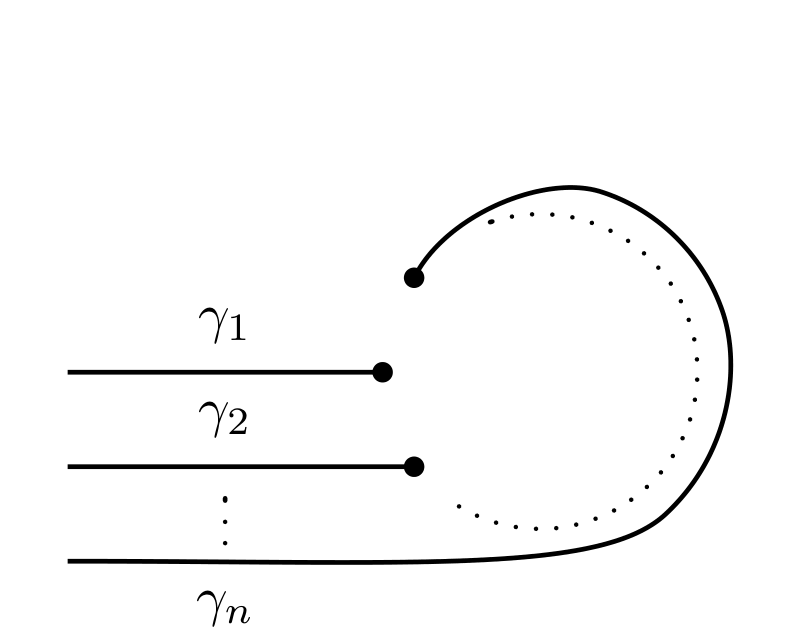
\includegraphics[width=\textwidth]{figures/fig13.1.png}
    \figtitle{13.1}{消没路径的临界集}
  \end{minipage}\hfill
  \begin{minipage}[b]{0.52\textwidth}
    \centering
    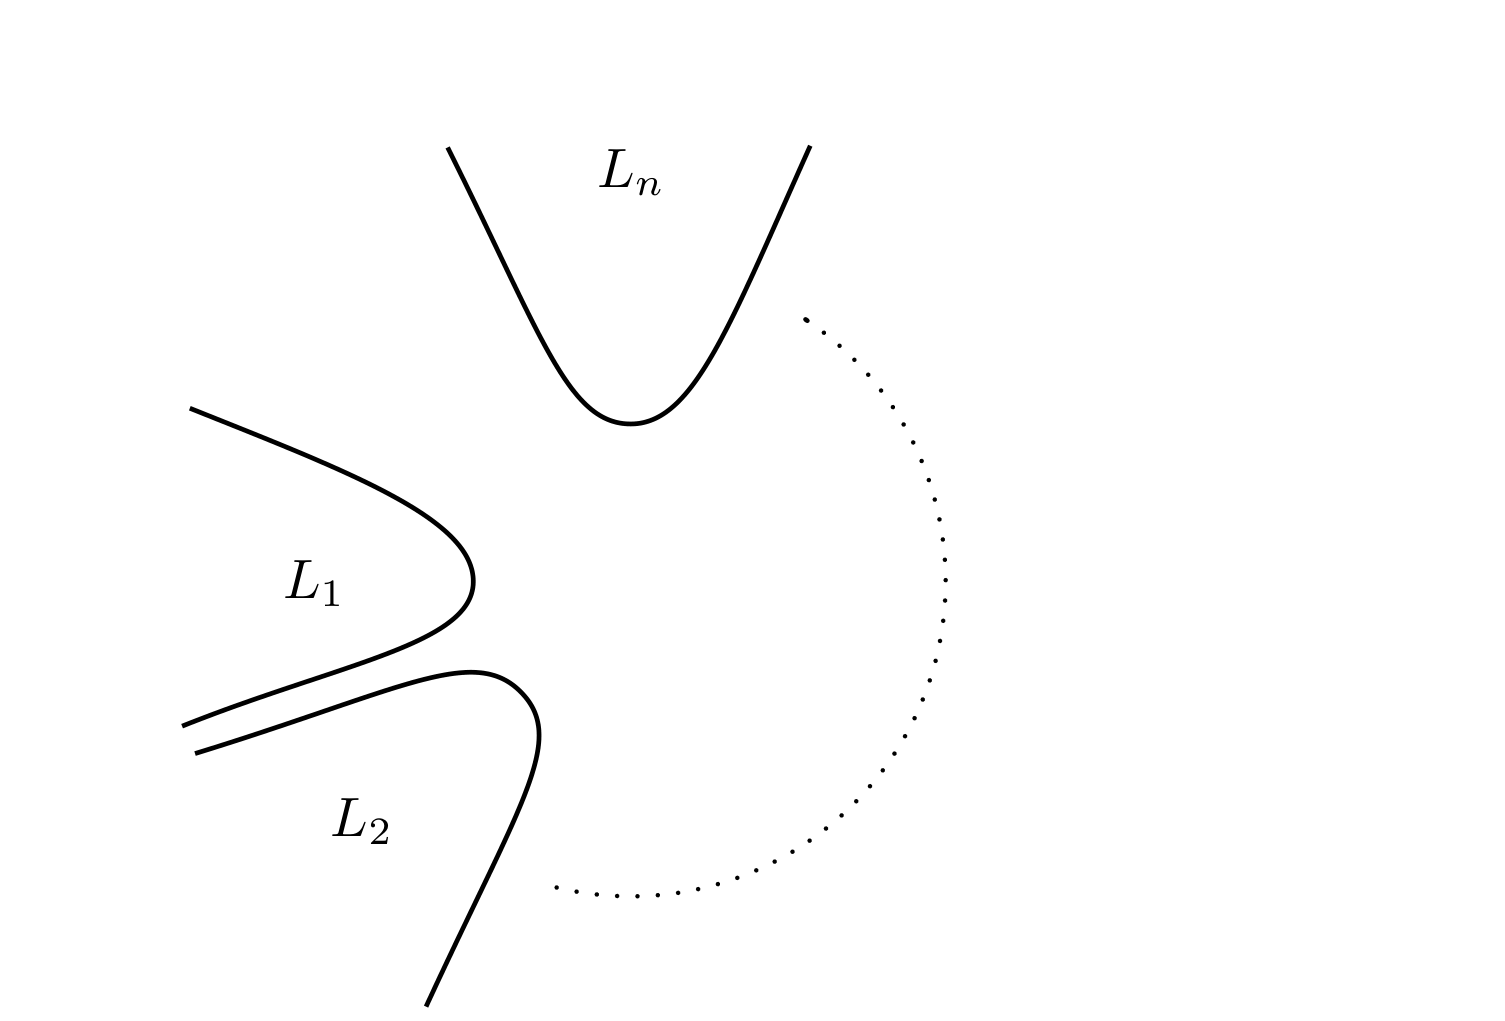
\includegraphics[width=\textwidth]{figures/fig13.2.png}
    \figtitle{13.2}{Lefschetz 穿透的特殊基}
  \end{minipage}
\end{figure}

\section{矩阵因子化}

对 Gorenstein 分次环\footnote{对 Abel 群 $H$，称给定了满足 $A_h\cdot A_{h'}\subset A_{h+h'}$ 的直和分解 $A=\bigoplus_{h\in H}A_h$ 的环为 $H$ 分次环（$H$-graded ring），或简称为分次环（graded ring）。对分次环而言，「所有素理想处的局部化都是 Gorenstein 局部环」与「所有齐次素理想处的局部化都是 Gorenstein 局部环」等价，满足这一条件的分次环称为 Gorenstein 分次环。} $R$，把有限生成分次 $R$-模构成的 Abel 范畴记为 $\mathrm{gr}\,R$，并把 $D^b\mathrm{gr}\,R$ 作为其有界导出范畴。$D^b\mathrm{gr}\,R$ 的对象若与投射模的有界复形拟同构，则称为完美复形（perfect complex）。把 $D^b\mathrm{gr}\,R$ 中由完美复形构成的满子范畴记作 $D^{\mathrm{perf}}\mathrm{gr}\,R$，称为完美导出范畴（perfect derived category）。有界导出范畴关于完美导出范畴的商\footnote{设 $\cT$ 为三角范畴，$\cN$ 为 $\cT$ 的满三角子范畴。把 $\cT$ 对使映射锥落入 $\cN$ 的态射集合进行局部化，便可再次得到三角范畴。称之为 $\cT$ 关于 $\cN$ 的 Verdier 商（Verdier quotient），记作 $\cT/\cN$。Keller [Dri04] 与 Drinfeld [Kel99] 证明了：增广三角范畴的 Verdier 商仍是增广三角范畴。} 称为稳定导出范畴（stable derived category）或奇点范畴（singularity category），并用
\begin{equation}
  D^b_{\mathrm{sing}}(\mathrm{gr}\,R) := D^b\mathrm{gr}\,R/D^{\mathrm{perf}}\mathrm{gr}\,R
  \tag{14.1}
\end{equation}
表示 [Buc87]。

% [Tutor Note: 原文脚注 54 的文献标记「Keller [Dri04] や Drinfeld [Kel99]」疑为张冠李戴
%  （[Dri04] 应为 Drinfeld、[Kel99] 应为 Keller）；此处按原文保留，请审校确认。]

正则分次环\footnote{对分次环而言，「所有素理想处的局部化都是正则局部环」与「所有齐次素理想处的局部化都是正则局部环」等价，满足这一条件的分次环称为正则分次环。} $S$ 与非零齐次元 $f\in S$ 给出的商环 $R:=S/(f)$ 是 Gorenstein 分次环的典型例子。此时稳定导出范畴可用 [Eis80] 引入的矩阵因子化（matrix factorization）具体描述\footnote{自由 $S$-模的无限序列 $K^{\bullet}=\left\{\cdots\to K^i\xrightarrow{k^i}K^{i+1}\xrightarrow{k^{i+1}}K^{i+2}\to\cdots\right\}$，若对任意 $i\in\Z$ 有 $K^{i+2}\cong K^i$ 且 $k^{i+1}\circ k^i=W$，则称为矩阵因子化（matrix factorization）。与复形的情形同样，矩阵因子化自然地构成微分分次范畴。关于矩阵因子化的解说，例如可参见 [Yos90]。}。

作为例子，考虑 $S:=\C[x]$、$f:=x^{n+1}$、$R:=S/(f)$ 的情形，则 $(E_i:=R/(x)(-i+1))_{i=1}^n$ 构成 $D^b_{\mathrm{sing}}(\mathrm{gr}\,R)$ 的完备例外序列，且它们之间的态射满足
\begin{equation}
  \Ext^k(E_i,E_j)\cong
  \begin{cases}
    \C\cdot\id_{S_i}, & i=j\ \text{且}\ k=0,\\
    \C, & j=i+1\ \text{且}\ k=1,\\
    0, & \text{其他}
  \end{cases}
  \tag{14.2}
\end{equation}
这一点容易看出 [Tak05, Orl09]。

% [Tutor Note: 原文 (14.2) 中的「id_{S_i}」疑为「id_{E_i}」之笔误（E_i 才是例外序列的元素），
%  此处按原文保留，请审校确认。]

\section{可逆多项式}

对以自然数为元素的 $n\times n$ 矩阵 $A$，定义 $n$ 元多项式 $f\in\C[x_1,\ldots,n]$ 为
\begin{equation}
  f=\sum_{i=1}^{n}x_1^{a_{i1}}\cdots x_n^{a_{in}}
  \tag{15.1}
\end{equation}
注意，$f$ 的非零系数可以通过把变量 $x_i$ 适当地乘以常数而规范化为 1。当 $A$ 为可逆矩阵、且 $f$ 在原点具有孤立临界点时，称 $f$ 为可逆多项式（invertible polynomial）。对 $f\in\C[x_1,\ldots,x_n]$ 与 $g\in\C[y_1,\ldots,y_m]$，称 $f+g\in\C[x_1,\ldots,x_n,y_1,\ldots,y_m]$ 为 $f$ 与 $g$ 的 Sebastiani–Thom 和（Sebastiani–Thom sum）[ST71]。一般而言，可逆多项式可由若干下述类型的 Sebastiani–Thom 和给出 [AGZV85, KS92]：

% [Tutor Note: 原文「C[x_1,\ldots,n]」中末项漏写了下标 x，应为 C[x_1,\ldots,x_n]；此处按原文保留，请审校确认。]

\begin{itemize}
  \item Fermat 型（Fermat type）：$f=x^p$
  \item 链型（chain type）：$f=x_1^{p_1}x_2+x_2^{p_2}x_3+\cdots+x_{n-1}^{p_{n-1}}x_n+x_n^{p_n}$
  \item 环型（loop type）：$f=x_1^{p_1}x_2+x_2^{p_2}x_3+\cdots+x_{n-1}^{p_{n-1}}x_n+x_n^{p_n}x_1$
\end{itemize}

对给定的可逆多项式，环 $\C[x_1,\ldots,x_n]/f$ 具有由 $(n+1)$ 个生成元 $\vec x_1,\ldots,\vec x_n,\vec c$ 与 $n$ 个关系式
\begin{equation}
  a_{i1}\vec x_1+\cdots+a_{in}\vec x_n=\vec c,\qquad i=1,\ldots,n
  \tag{15.2}
\end{equation}
定义的秩 1 的 Abel 群 $L$ 所给出的自然分次。这个 $L$ 是由
\begin{equation}
  K:=\left\{(\alpha_1,\ldots,\alpha_n)\in(\C^\times)^n\;\middle|\;
  \alpha_1^{a_{11}}\cdots\alpha_n^{a_{1n}}=\cdots=\alpha_1^{a_{n1}}\cdots\alpha_n^{a_{nn}}\right\}
  \tag{15.3}
\end{equation}
定义的群的特征标群。最大对角对称群（the group of maximal diagonal symmetries）$G_{\max}$ 定义为映射
\begin{equation}
  K\to\C^\times,\qquad (\alpha_1,\ldots,\alpha_n)\mapsto\alpha_1^{a_{11}}\cdots\alpha_n^{a_{1n}}
  \tag{15.4}
\end{equation}
的核：
\begin{equation}
  1\to G_{\max}\to K\to\C^\times\to1.
  \tag{15.5}
\end{equation}
(15.5) 诱导出特征标群的正合列
\begin{equation}
  0\to\Z\to L\to G_{\max}^{\vee}\to0
  \tag{15.6}
\end{equation}
这里，
\begin{equation}
  G_{\max}^{\vee}:=\Hom(G_{\max},\C^\times)
  \tag{15.7}
\end{equation}
与 $G_{\max}$ 之间有一个并非典范（canonical）的同构。把 $A$ 的逆矩阵置为
\begin{equation}
  A^{-1}=
  \begin{pmatrix}
    \varphi_1^{(1)} & \varphi_1^{(2)} & \cdots & \varphi_1^{(n)}\\
    \varphi_2^{(1)} & \varphi_2^{(2)} & \cdots & \varphi_2^{(n)}\\
    \vdots & \vdots & \ddots & \vdots\\
    \varphi_n^{(1)} & \varphi_n^{(2)} & \cdots & \varphi_n^{(n)}
  \end{pmatrix}
  \tag{15.8}
\end{equation}
则 $G_{\max}$ 由
\begin{equation}
  \rho_k:=\left(\exp\left(2\pi\sqrt{-1}\varphi_1^{(k)}\right),\ldots,
  \exp\left(2\pi\sqrt{-1}\varphi_n^{(k)}\right)\right)
  \tag{15.9}
\end{equation}
生成。对 $i=1,\ldots,n$ 置
\begin{equation}
  \varphi_i\colon\varphi_i^{(1)}+\cdots+\varphi_i^{(n)}
  \tag{15.10}
\end{equation}
并令群同态 $\varphi\colon\C^\times\to K$ 由
\begin{equation}
  \varphi(\alpha):=\left(\alpha^{\ell\varphi_1},\ldots,\alpha^{\ell\varphi_n}\right)
  \tag{15.11}
\end{equation}

% CHUNK c06 DONE pages p022–p023

% c07 = p024–p028（第 16–17 节；p024 顶部为第 15 节正文的续篇）
% [Tutor Note: p024 顶部承接 p023 末尾「群の準同型 φ: ℂ^× → K を (15.11) で定義する。」一句，
%  故本 chunk 以「来定义。」起句；第 15 节的续文到 (15.18) 与转置镜像对称的说明为止，
%  其后才是第 16 节标题。]

来定义。但 $\ell$ 是对所有 $i=1,\dots,n$ 使 $\ell\varphi_i$ 为整数的最小非负整数。此时 $\varphi$ 是单射，将其余核记作 $\overline{G}_{\max}$；

\begin{equation}
  1 \to \C^{\times} \xrightarrow{\ \varphi\ } K \to \overline{G}_{\max} \to 1. \tag{15.12}
\end{equation}

$W$ 通过

\begin{equation}
  \deg x_i = \ell\varphi_i,\quad i=1,\dots,n \tag{15.13}
\end{equation}

而具有 $\Z$-分次。由于 $f$ 在原点处有孤立临界点，加权超曲面

\begin{equation}
  Y := \bigl\{[x_1:\cdots:x_n]\in\PP(\ell\varphi_1,\dots,\ell\varphi_n) \bigm| f(x_1,\dots,x_n)=0\bigr\} \tag{15.14}
\end{equation}

是光滑的 Deligne–Mumford 栈。$Y$ 的典范丛成为平凡丛的充要条件是

\begin{equation}
  \deg x_1 + \cdots + \deg x_n = \ell \tag{15.15}
\end{equation}

成立。$\operatorname{Im}\varphi\cap G$ 由

\begin{equation}
  J := \bigl(\exp(2\pi\sqrt{-1}\varphi_1),\dots,\exp(2\pi\sqrt{-1}\varphi_n)\bigr) \tag{15.16}
\end{equation}

生成。假设 $J\in G$，令 $\overline{G} := G/\langle J\rangle$，并把自然满射 $K\to\overline{G}_{\max}$ 下 $\overline{G}$ 的原像记作 $M$。此外，把 $M$ 的特征标群记作 $H$。此时，Calabi–Yau 栈 $[Y/\overline{G}]$ 与 Landau–Ginzburg 轨形 $(f,G)$（或 $(f,M)$）\footnote{代数流形上的全纯函数 $f\colon V\to\C$ 与作用在 $V$ 上且使 $f$ 不变的群 $G$ 所成的组 $(f,G)$，这里称为 Landau–Ginzburg 轨形。}密切相关这一猜想称为 Calabi–Yau/Landau–Ginzburg 对应（Calabi–Yau/Landau–Ginzburg correspondence）。这至少是回溯到 [Gep87] 的古老想法，而最近的发展例如有 [Orl09, CR10, CR11, CIR14] 等。

可逆多项式 $f$ 的转置（transpose）由

\begin{equation}
  \check{f} := \sum_{i=1}^{n} x_1^{a_{1i}}\cdots x_n^{a_{ni}} \tag{15.17}
\end{equation}

定义。$\check{f}$ 的最大对角对称性群 $\check{G}_{\max}$ 由 $(A^T)^{-1}=(A^{-1})^T$ 的列向量 $\check{\rho}_i$ 生成。对 $G_{\max}$ 的子群 $G$，$G$ 的转置 $\check{G}$ 由

\begin{equation}
  \check{G} := \left\{\prod_{i=1}^{n}\check{\rho}_i^{r_i} \ \middle|\
    \text{对任意 } \prod_{i=1}^{n}\rho_i^{a_i}\in G \text{，均有 } (r_1\ \cdots\ r_n)\,A^{-1}
    \begin{pmatrix} a_1\\ \vdots\\ a_n\end{pmatrix}\in\Z \right\} \tag{15.18}
\end{equation}

定义（见 [Kra]）。对应 $G\leftrightarrow\check{G}$ 分别把 $G_{\max}$ 与 $\{e\}$、把 $\langle J\rangle$ 与 $G_{\max}\cap SL_n(\C)$ 互换。此时，Landau–Ginzburg 模型 $(f,G)$ 与 $(\check{f},\check{G})$ 互为镜像，这就是 Berglund–Hübsch [BH93] 的转置镜像对称（transposition mirror symmetry）。

\section{箭图及其表示}

同调镜像对称的证明方针大致分为两种。一种是用 Fourier 变换那样的几何方法定义函子，并证明它是满忠实且本质满射的；另一种则是，对每个范畴找出其生成元，使这些生成元的自同构代数作为微分分次代数或 A∞ 代数拟同构。这些方法类似于：要证明两个环同构，先作出同态，再证明它既满又单；也类似于在生成元之间建立对应，再证明关系式一致。

% [Tutor Note: 原文作「自己同型代数」，按上下文疑为「自己準同型代数」（自同态代数）之笔误，此处按原文译作「自同构代数」，请审校确认。]

给定预完备的增广三角范畴 $\cD$ 的紧生成元 $E$ 时，对于 $\cA := \operatorname{hom}_{\cD}(E,E)$，函子

\begin{equation}
  \operatorname{RHom}_{\cD}(E,-)\colon \cD \to D\cA \tag{16.1}
\end{equation}

及其伴随函子

\begin{equation}
  (-)\otimes_{\cA} E\colon D\cA \to \cD \tag{16.2}
\end{equation}

给出范畴等价\footnote{虽然也有人强调这与 Fourier–SYZ 变换（或族的 Floer 上同调）的类似性，但有一个显著差异：拉格朗日环面纤维化即使把所有纤维合起来也不生成导出范畴（在镜像一侧看，点层不用说导出范畴，就连 $K$ 群也不生成）。}。若 $\cA$ 是非循环的（acyclic，即对 $i\ne 0$ 有 $H^i(\cA)=0$），则 $D\cA$ 等价于 $A := H^0(\cA)$ 上模的导出范畴。

由顶点（vertex）的集合 $Q_0$、箭（arrow）的集合 $Q_1$，以及对每个箭赋予其起点（source）与终点（target）的映射 $s,t\colon Q_1\to Q_0$ 组成的组 $Q := (Q_0,Q_1,s,t)$ 称为箭图（quiver）。当 $Q_0$ 与 $Q_1$ 都是有限集时，称 $Q$ 是有限的（finite）。对正整数 $k$，长度（length）为 $k$ 的路（path）是指箭的序列 $(a_k,\dots,a_2,a_1)$，且对任意 $i=1,\dots,k-1$ 满足 $s(a_{i+1})=t(a_i)$。另外，对每个顶点 $v\in Q_0$，考虑以 $v$ 为起点、以 $v$ 为终点、长度为 $0$ 的元素 $e_v$，这也称为路。在由路张成的向量空间上赋予乘法

\begin{equation}
  (a_k,\dots,a_1)\cdot(b_l,\dots,b_1) =
  \begin{cases}
    (a_k,\dots,a_1,b_l,\dots,b_1) & s(a_1)=t(b_l),\\
    0 & \text{其他}
  \end{cases} \tag{16.3}
\end{equation}

所得的代数称为路代数（path algebra），记作 $\C Q$。附着于顶点的长度为 $0$ 的路是这个代数的幂等元。路代数 $\C Q$ 具有由路长给出的自然分次 $\C Q=\bigoplus_{n=0}^{\infty}(\C Q)_n$。箭图 $Q$ 与其路代数的双边理想 $I\subset\C Q$ 组成的组 $\Gamma := (Q,I)$ 称为带关系箭图（quiver with relations），$\C\Gamma := \C Q/I$ 称为它的路代数。以下假设箭图的关系式都含于由长度 $2$ 以上的元素构成的子模中；

\begin{equation}
  I \subset (\C Q)_{\ge 2} := \bigoplus_{n=2}^{\infty}(\C Q)_n. \tag{16.4}
\end{equation}

对带关系箭图 $\Gamma$，其路代数 $\C\Gamma$ 上的模称为 $\Gamma$ 的表示（representation）。给出带关系箭图的表示，等价于给出：对应各顶点 $v$ 的线性空间 $M_v$ 与对应各箭 $a$ 的线性映射 $\varphi_a\in\Hom(M_{s(a)},M_{t(a)})$ 所成的组 $\bigl((M_v)_{v\in Q_0},(\varphi_a)_{a\in Q_1}\bigr)$，且满足关系式。

把由对应顶点的幂等元生成的半单代数记作

\begin{equation}
  \C^{Q_0} := \bigoplus_{v\in Q_0}\C e_v \tag{16.5}
\end{equation}

则带关系箭图的路代数是半单代数 $\C^{Q_0}$ 上的代数。反之，给定半单代数 $\C^{Q_0}$ 上的代数 $A$ 时，存在线性空间的直和分解 $A=\bigoplus_{v,w\in Q_0}e_v A e_w$，于是从各直和项中适当选取 $A$ 的生成元并置为 $Q_1$，当 $a\in Q_1$ 是 $e_v A e_w$ 的元素时定义 $s(a):=w$、$t(a):=v$，便得到箭图 $Q := (Q_0,Q_1,s,t)$。由构造，存在从 $\C Q$ 到 $A$ 的自然满射，取其核为 $I$ 并令 $\Gamma := (Q,I)$，则 $\C\Gamma$ 与 $A$ 自然同构。

对非循环的生成元 $E=E_1\oplus\cdots\oplus E_n$，准备与直和项个数相同数目的顶点并置 $Q_0 := \{v_1,\dots,v_n\}$，则通过把 $e_i := e_{v_i}$（$i=1,\dots,n$）送到 $\id_{E_i}\subset A$，$E$ 的自同态代数 $A$ 成为半单代数 $\C^{Q_0}$ 上的代数，从而可表示为适当的带关系箭图的路代数。

设 $\Gamma$ 为带关系箭图，$A := \C\Gamma$ 为其路代数。对任意顶点 $v\in Q_0$，把幂等元 $e_v\in A$ 生成的 $A$ 的右子模记作 $P_v := e_v A$。由 $1=\sum_{v\in Q_0}e_v$ 得 $A\cong\bigoplus_{v\in Q_0}P_v$，因此 $P_v$ 是 $A$ 的直和项，从而是射影模。当带关系箭图来自非循环的生成元 $E=E_1\oplus\cdots\oplus E_n$ 时，由范畴等价 (16.1)，$E_i$ 被送到 $P_i := P_{v_i}$。另一方面，给定顶点 $v$ 时，对顶点 $w$ 把线性空间定义为

\begin{equation}
  M_w =
  \begin{cases}
    \C & w=v,\\
    0 & \text{其他}
  \end{cases} \tag{16.6}
\end{equation}

并对所有箭 $a\in Q_1$ 令 $\varphi_a=0$，则 $\bigl((M_w)_{w\in Q_0},(\varphi_a)_{a\in Q_1}\bigr)$ 是 $\Gamma$ 的表示；把它记作 $S_v$，称为附着于 $v$ 的单模。$A$-模 $S_v$ 的射影分解的首项为

\begin{equation}
  \cdots \to \bigoplus_{t(a)=v}P_{s(a)} \to P_v \to S_v \to 0 \tag{16.7}
\end{equation}

给出，其核来自 $A$ 的关系式。把这个射影分解用函子 $\Hom(-,S_w)$ 送出，便可看出：$\Ext^1(S_v,S_w)$ 的基对应于从 $w$ 到 $v$ 的箭，$\Ext^2(S_v,S_w)$ 的基对应于从 $w$ 到 $v$ 的路的关系式。

不具有非平凡直和分解的对象称为不可分解的（indecomposable），不具有平凡子对象的对象称为不可约的（irreducible），除恒等映射的常数倍以外没有自同态的对象称为单的（simple）。又，单且非循环的对象称为例外对象（exceptional object）。若例外对象的序列 $(E_i)_{i=1}^n$ 对任意 $i>j$ 与任意 $k\in\Z$ 满足 $\Ext^k(E_i,E_j)=0$，则称为例外序列（exceptional collection）。非循环的例外序列称为强例外序列（strong exceptional collection）。$\bigoplus_{i=1}^n E_i$ 为生成元的例外序列称为完备例外序列（full exceptional collection）。

起点与终点一致的路称为有向循环（oriented cycle）。又，不含任何有向循环的箭图称为有向箭图（directed quiver）。完备强例外序列的全同态代数（total morphism algebra）$A := \bigoplus_{i,j=0}^n \Hom(E_i,E_j)\cong\End\bigl(\bigoplus_{i=0}^n E_i\bigr)$ 同构于带关系有向箭图的路代数。

% [Tutor Note: 原文作 ⊕_{i,j=0}^n Hom(E_i,E_j) ≅ End(⊕_{i=0}^n E_i)，而例外序列 (E_i)_{i=1}^n 的指标自 1 起，疑「0」应为「1」，此处按原文保留。]

在有向箭图的表示中，单模序列 $(S_n,S_{n-1},\dots,S_1)$ 构成完备例外序列，并且

\begin{equation}
  \Ext^k(P_i,S_j) =
  \begin{cases}
    \C & i=j \text{ 且 } k=0,\\
    0 & \text{其他}
  \end{cases} \tag{16.8}
\end{equation}

在这个意义上，它与射影模组成的强完备例外序列 $(P_i)_{i=1}^n$ 互为对偶。完备例外序列 $(S_i)_{i=n}^1$ 绝不会成为强例外序列，但若 $A$ 是 Koszul 代数（Koszul algebra），则在导出范畴中平移次数所得的序列 $(S_i[-i])_{i=n}^1$ 是强例外序列，且其全同态代数为 $A$ 的 Koszul 对偶代数（Koszul dual algebra）。在这个意义上，$(S_i[i])_{i=n}^1$ 的作为微分分次代数或 A∞ 代数的全同态代数，给出 $A$ 的 Koszul 对偶代数的推广。

作为箭图的例子，考虑由

\begin{equation}
  v_1 \xleftarrow{a_1} v_2 \xleftarrow{a_2} \cdots \xleftarrow{a_{n-1}} v_n \tag{16.9}
\end{equation}

给出的箭图 $Q$。它有 $n$ 个顶点 $Q_0=\{v_1,\dots,v_n\}$ 与 $n-1$ 支箭 $Q_1=\{a_1,\dots,a_{n-1}\}$，且对任意 $i=1,\dots,n-1$ 有 $s(a_i)=v_{i+1}$ 且 $t(a_i)=v_i$。对 $i,j=1,\dots,n$ 定义路 $a_{ij}$ 为

\begin{equation}
  a_{ij} :=
  \begin{cases}
    a_i a_{i+1}\cdots a_{j-1} & i<j,\\
    e_{v_i} & i=j,\\
    0 & i>j
  \end{cases} \tag{16.10}
\end{equation}

则路代数中的乘法由

\begin{equation}
  a_{ij}a_{kl} =
  \begin{cases}
    a_{il} & j=k,\\
    0 & \text{其他}
  \end{cases} \tag{16.11}
\end{equation}

给出。把除 $(i,j)$ 分量外全为 $0$、该分量为 $1$ 的 $n\times n$ 矩阵记作 $E_{ij}$，则通过映射 $a_{ij}\mapsto E_{ij}$，$Q$ 的路代数 $A := \C Q$ 同构于 $n$ 次上三角矩阵代数。由射影模 $P_i := e_i A$ 组成的强完备例外序列 $(P_n,P_{n-1},\dots,P_1)$ 的对偶序列由单模 $S_i := \C e_i$ 组成，而它们之间射构成的线性空间为

\begin{equation}
  \Ext^k(S_i,S_j) \cong
  \begin{cases}
    \C\cdot\id_{S_i} & i=j \text{ 且 } k=0,\\
    \C & j=i+1 \text{ 且 } k=1,\\
    0 & \text{其他}
  \end{cases} \tag{16.12}
\end{equation}

分次代数 $A := \bigoplus_{k=0}^{\infty}\bigoplus_{i,j=1}^n \Ext^k(S_i,S_j)$ 的乘法结构，容易看出由作为分次线性空间的结构 (16.12) 唯一确定。进一步，微分分次代数 $\cA$ 是形式的这一事实也容易由 (16.12) 推出。一般地，分次代数 $A$ 的增广\footnote{对给定的分次代数 $A$，上同调代数为与 $A$ 同构的微分分次代数 $\cA$ 称为 $A$ 的增广（enhancement）。} 唯一的现象称为内在形式性（intrinsic formality）。

把 Fukaya–Seidel 范畴中的射空间 (13.12) 与矩阵因子化范畴中的 (14.2)，同 (16.12) 所给分次代数的内在形式性结合起来，便对 $f := x^{n+1}-ax$ 与 $\check{f} := x^{n+1}$ 得到增广三角范畴的等价

\begin{equation}
  D^b\cF(f) \cong D^b_{\mathrm{sing}}\bigl(\operatorname{gr}\C[x]/(\check{f})\bigr) \tag{16.13}
\end{equation}

这就是关于 $A_n$ 奇点的同调镜像对称。类似的结果被猜想对更一般的可逆多项式也成立，并已在若干情形得到证明；关于这一点，例如可参见 [FU]。

\section{环面 Fano 流形的同调镜像对称}

在关于 Calabi–Yau 流形以外的流形的同调镜像对称中，研究得最深入的是环面 Fano 流形的情形。环面 Fano 流形的镜像是 Landau–Ginzburg 模型；由于这一明显的不对称性，按在哪一侧考虑辛几何而有两个版本。

环面 Fano 流形 $X$ 由凸格多面体\footnote{有限个格点的凸包（convex hull）称为凸格多面体（convex lattice polytope）。}决定，其复结构没有模空间。另一方面，辛结构在把 $X$ 构造为辛向量空间在环面作用下的辛商时，会随动量映射的值（等位集）的选取而变化，因而具有 $b_2=\dim H^2(X,\R)$ 维的模空间。这个模空间在镜像的 Landau–Ginzburg 模型中对应于势 $W$ 的系数。

同调镜像对称的一个版本是

\begin{equation}
  D^b\operatorname{coh}X \cong D^b\cF(W) \tag{17.1}
\end{equation}

而另一个版本是

\begin{equation}
  D^{\pi}\cF(X) \cong D^b_{\mathrm{sing}}(W) \tag{17.2}
\end{equation}

在无模空间依赖性这个意义上，(17.1) 更容易；但对一般的辛结构，期望 (17.2) 中出现的两个范畴都是半单的（即成为向量空间复形范畴的直和），在这个意义上 (17.2) 更容易。不过，给出 $X$ 的 Gromov–Witten 不变量与势 $W$ 的振荡积分之间关系、并应作为推论导出的经典镜像对称，其主张属于 (17.2) 一方。对未必是 Fano 流形的一般紧辛环面流形，(17.2) 的证明已由 Abouzaid–Fukaya–Oh–Ohta–Ono 预告。此外，关于此情形下同调镜像对称与经典镜像对称的关系，在 [FOOO] 中有详细讨论。不过，即便在这种情况下，也尚未从增广三角范畴的等价导出经典镜像对称。

以下讨论 (17.1)。

设 $\bm{N}$ 为秩 $n$ 的自由 Abel 群，其对偶 Abel 群记作 $\bm{M} := \Hom(\bm{N},\Z)$。设 $\Delta\subset\bm{N}_{\R} := \bm{N}\otimes\R$ 为凸格多面体，并假设 $\Delta$ 以原点为内点。把 $\Delta$ 的格点集记作 $A := \Delta\cap\bm{N}$，并把以 $\Delta$ 为 Newton 多面体的洛朗多项式记作

\begin{equation}
  W = \sum_{n\in A}a_n x^n \tag{17.3}
\end{equation}

这里若系数 $(a_n)_{n\in A}\in\C^A$ 取得足够一般，$W$ 所定义的映射 $\bm{M}^{\times}_{\C} := \Spec\C[\bm{N}]\to\C$ 给出 Lefschetz 纤维化。(17.1) 的右边就是如此得到的 Lefschetz 纤维化的 Fukaya–Seidel 范畴。但定义域 $\bm{M}^{\times}_{\C}\cong(\C^{\times})^n$ 上要赋予以 $-\sqrt{-1}/2\sum_{i=1}^n \dd x_i\wedge \dd\bar{x}_i/|x_i|^2$ 为辛形式的自然辛结构。

把 $\Delta$ 的顶点集记作 $\{n_i\}_{i=1}^r$，并定义映射 $\phi\colon\Z^r\to\bm{N}$ 为 $\phi(e_i) := n_i$。其中把 $\Z^r$ 的标准基记作 $(e_i)_{i=1}^r$。进一步，选取并固定 $\Delta$ 的边界（即余维 $1$ 的面的并集）的一个三角剖分 $\Sigma$，使其顶点集与 $\Delta$ 的顶点集一致。若存在某 $\{i_1,\dots,i_k\}\subset\{1,\dots,r\}$，使得 $z_{i_1}=\cdots=z_{i_k}=0$，但由 $\{v_{i_1},\dots,v_{i_k}\}$ 张成的单纯形不属于 $\Sigma$，这样的点 $(z_1,\dots,z_r)\in\C^r$ 的集合称为 Stanley–Reisner 轨迹（Stanley–Reisner locus），记作 $\mathrm{SR}(\Sigma)$。

% [Tutor Note: 原文此处作 {v_{i_1},…,v_{i_k}}，但上文把 Δ 的顶点记为 n_i，疑为记号混用或笔误；此处按原文保留 v。]

$\phi$ 诱导的映射 $\phi_{\C^{\times}}\colon(\C^{\times})^r\to\bm{N}_{\C^{\times}}$ 的核 $K := \operatorname{Ker}\phi_{\C^{\times}}\subset(\C^{\times})^r$ 通过 $(\C^{\times})^r$ 对 $\C^r$ 的自然作用而作用于 $\C^r$；关于这个作用，把 $\C^r\setminus\mathrm{SR}(\Sigma)$ 的栈论意义下的商记作

\begin{equation}
  X_{\Sigma} := [(\C^r\setminus\mathrm{SR}(\Sigma))/K] \tag{17.4}
\end{equation}

并称为附着于 $\Sigma$ 的环面栈。此时，猜想 2.5 断言增广三角范畴的等价

\begin{equation}
  D^b\operatorname{coh}X_{\Sigma} \cong D^b\cF(W) \tag{17.5}
\end{equation}

的存在。$X_{\Sigma}$ 一般是环面弱 Fano 栈\footnote{典范丛为 nef 且丰富的栈称为弱 Fano 栈。}。$X_{\Sigma}$ 成为代数流形的充要条件是 $\Sigma$ 为幺模的（即 $\Sigma$ 的任意单纯形都可通过 $GL_n(\Z)\ltimes\Z^n$ 的作用移到标准单纯形），而 $X_{\Sigma}$ 成为 Fano 的充要条件是 $\Sigma$ 的所有面都是 $\Delta$ 的面。$X_{\Sigma}$ 的同构类依赖于单纯剖分 $\Sigma$ 的选取，但导出范畴 $D^b\operatorname{coh}X_{\Sigma}$ 作为增广三角范畴的拟同构类仅由 $\Delta$ 决定 [Kaw05]。

作为例子，考虑 $\bm{N}:=\Z$ 是秩 $1$ 的 Abel 群、$\Delta_{a,b} := [-a,b]$ 是长度为 $a+b$ 的闭区间的情形。此时

\begin{equation}
  \phi_{\C^{\times}}\colon(\C^{\times})^2\to\C^{\times},\quad
  (\alpha,\beta)\mapsto\alpha^{-a}\beta^{b} \tag{17.6}
\end{equation}

而其核同构于 $\C^{\times}\times\Z/c\Z$，其中 $c := \gcd(a,b)$。$\partial\Delta$ 的单纯剖分是唯一的，Stanley–Reisner 轨迹为 $\bm{0} := \{(0,0)\}$。$K$ 在 $\C^2\setminus\bm{0}$ 上的作用在 $(1,0)$ 与 $(0,1)$ 处分别有同构于 $\Z/a\Z$ 与 $\Z/b\Z$ 的稳定化子。对应的环面栈记作

\begin{equation}
  \mathbb{X}_{a,b} := [(\C^2\setminus\bm{0})/K] \tag{17.7}
\end{equation}

若 $a$ 与 $b$ 互素，则 $\mathbb{X}_{a,b}$ 同构于 $\C^{\times}$ 通过作用 $(x,y)\mapsto(\alpha^a x,\alpha^b y)$ 在 $\C^2\setminus\bm{0}$ 上的商 $\PP(a,b) := [(\C^2\setminus\bm{0})/\C^{\times}]$。作为镜像，取

\begin{equation}
  W(x) = x^a - \frac{1}{x^b} \tag{17.8}
\end{equation}

则临界点由 $x^{a+b}=b/a$ 定义，其中一个是正实数。取 $\infty$ 为起点，选取连结临界值与 $\infty$ 的实轴上的半直线 $\gamma_1$ 作为消没路径，则对应的 Lefschetz 穿透 $L_1$ 成为 $x$ 平面的正实轴。令 $n=a+b$、$\zeta_n=\exp(2\pi\sqrt{-1}/n)$，对 $i\in\{1,\dots,n-1\}$，把用映射 $x\mapsto\zeta_n^i x$ 移动 $L_1$ 所得的记为 $\zeta_n^i L_1$，则它是沿 $\zeta_n^{ai}\gamma_1$ 的 Lefschetz 穿透。在紧集之外把 $\zeta_n^{ai}\gamma_1$ 形变为与正实轴平行，则 $\zeta_n^i L_1$ 在无穷远附近被旋转 $-\frac{2ai\pi}{n}$，在 $0$ 附近被旋转 $\frac{2bi\pi}{n}$。把这样得到的 Lefschetz 穿透记作 $L_{i+1}$，则 $(L_i)_{i=1}^n$ 成为 Lefschetz 穿透的特殊基。关于这个特殊基的 Fukaya–Seidel 范畴容易计算，若适当选取由 $\mathbb{X}$ 的线丛组成的完备强例外序列 $(\cL_i)_{i=1}^n$，则容易看出

% [Tutor Note: 原文此处作「Lefscheta 指貫」，疑为「Lefschetz 指貫」之笔误，正文按「Lefschetz 穿透」译出。]

\begin{equation}
  \Hom_{\mathfrak{Fuk}\,W}(L_i,L_j) \cong \Hom_{\mathbb{X}}(\cL_i,\cL_j) \tag{17.9}
\end{equation}

成立\footnote{若 $a$ 与 $b$ 互素，则可取 $\cL_i=\cO(i)$。若 $a$ 与 $b$ 不互素，则可描述为 $a$ 与 $b$ 互素情形的覆叠。}。

作为例子，考虑 $(a,b)=(1,1),(2,2),(3,5)$ 的情形。Lefschetz 穿透的特殊基分别如图 17.1、图 17.2 及图 17.3 所示，对应的箭图分别由 (17.10)、(17.11) 及 (17.12) 给出。注意在 $(a,b)=(1,1)$ 的情形 $\mathbb{X}=\PP^1$，而在 $(a,b)=(2,2)$ 的情形 $\mathbb{X}$ 是它的覆叠。

\begin{equation}
  1 \rightrightarrows 2 \tag{17.10}
\end{equation}

% [Tutor Note: (17.10) 之后的箭图 (17.11)、(17.12) 与图 17.1–17.3 位于 p029（属 c08），本 chunk 至 p028 末的 (17.10) 为止。]

% tags: (15.12)–(15.18) 7 条 + (16.1)–(16.13) 13 条 + (17.1)–(17.10) 10 条 = 30 条
% CHUNK c07 DONE pages p024–p028

% ===== c08 第 18 节「半正交分解」 p029–p032 =====
% 页面图像上实际编号公式 42 条：(17.11)(17.12) + (18.1)–(18.40)。
% p029 上半页为第 17 节末尾的箭图 (17.11)(17.12) 与图 17.1–17.3；第 18 节标题自 p029 中部起。

\begin{equation}
  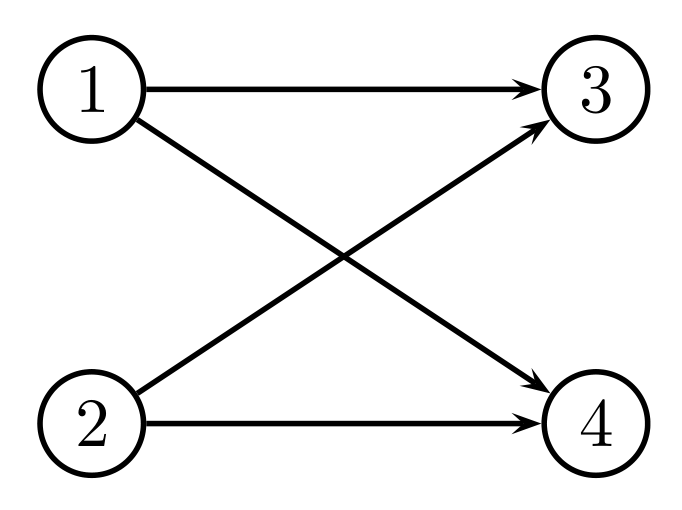
\includegraphics[width=0.24\textwidth]{figures/eq17.11.png}
  \tag{17.11}
\end{equation}

\begin{equation}
  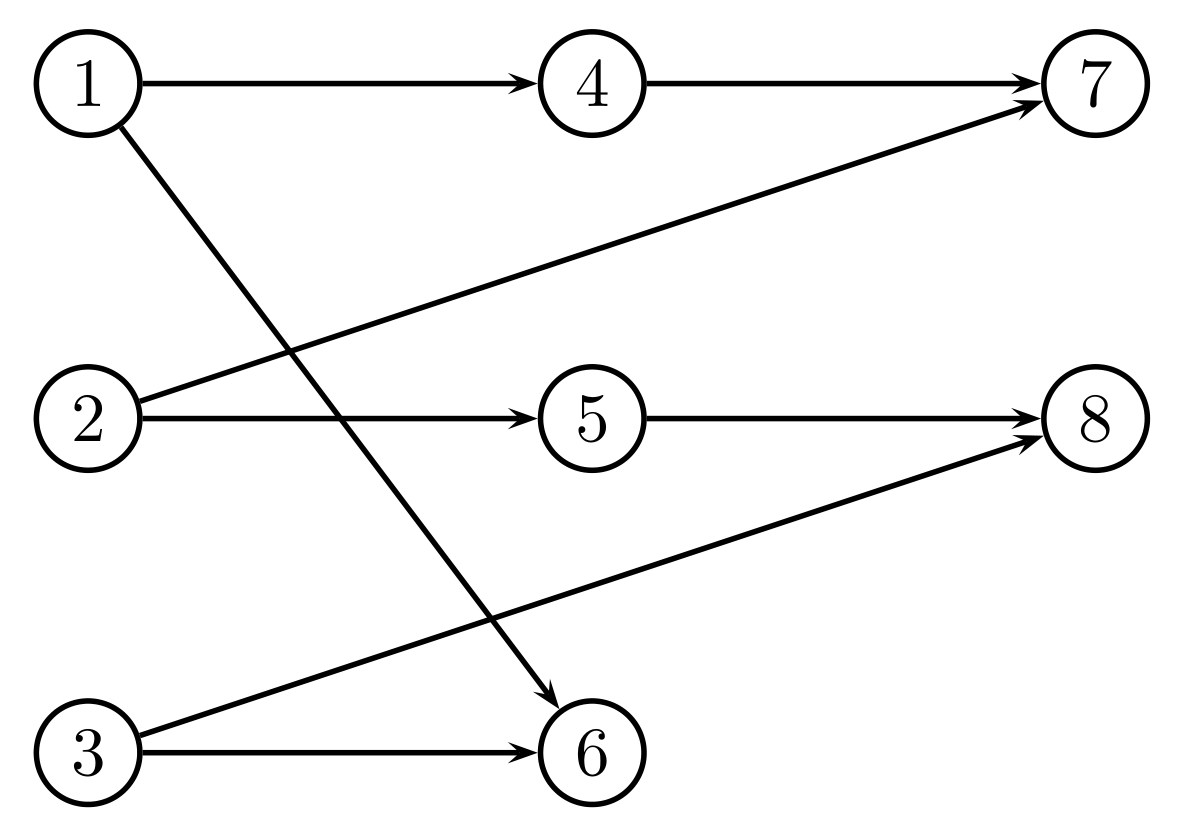
\includegraphics[width=0.41\textwidth]{figures/eq17.12.png}
  \tag{17.12}
\end{equation}

% [Tutor Note: (17.11)(17.12) 为箭图（quiver）示意，原书以图元绘制；preamble 未加载 tikz，故按页面裁图原样嵌入（work/figures/eq17.11.png、work/figures/eq17.12.png），节点编号与箭头方向均未改动。]

\begin{figure}[htbp]\centering
  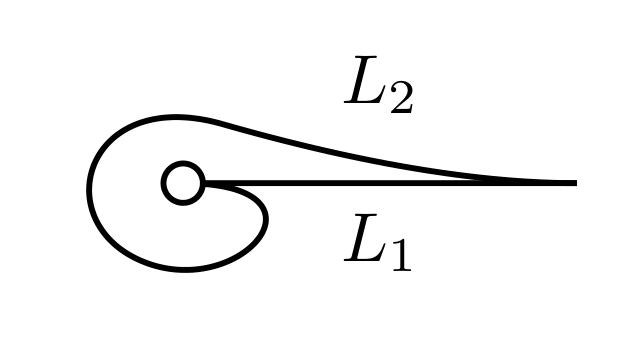
\includegraphics[width=0.28\textwidth]{figures/fig17.1.png}
  \figtitle{17.1}{$(a,b)=(1,1)$}
\end{figure}

\begin{figure}[htbp]\centering
  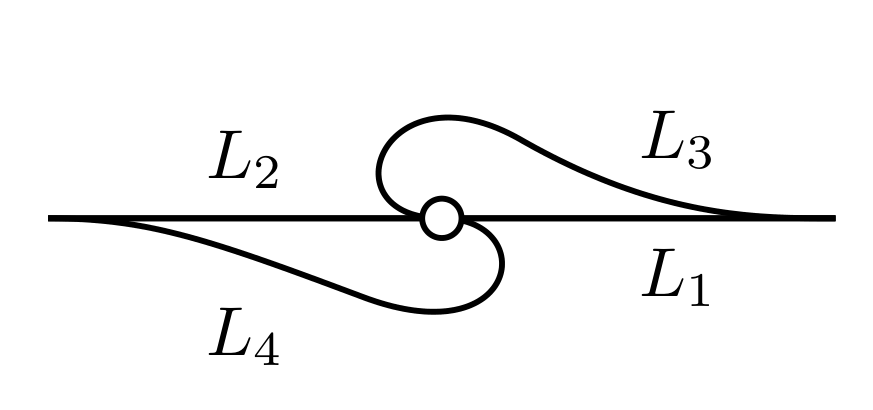
\includegraphics[width=0.34\textwidth]{figures/fig17.2.png}
  \figtitle{17.2}{$(a,b)=(1,1)$}
\end{figure}

\begin{figure}[htbp]\centering
  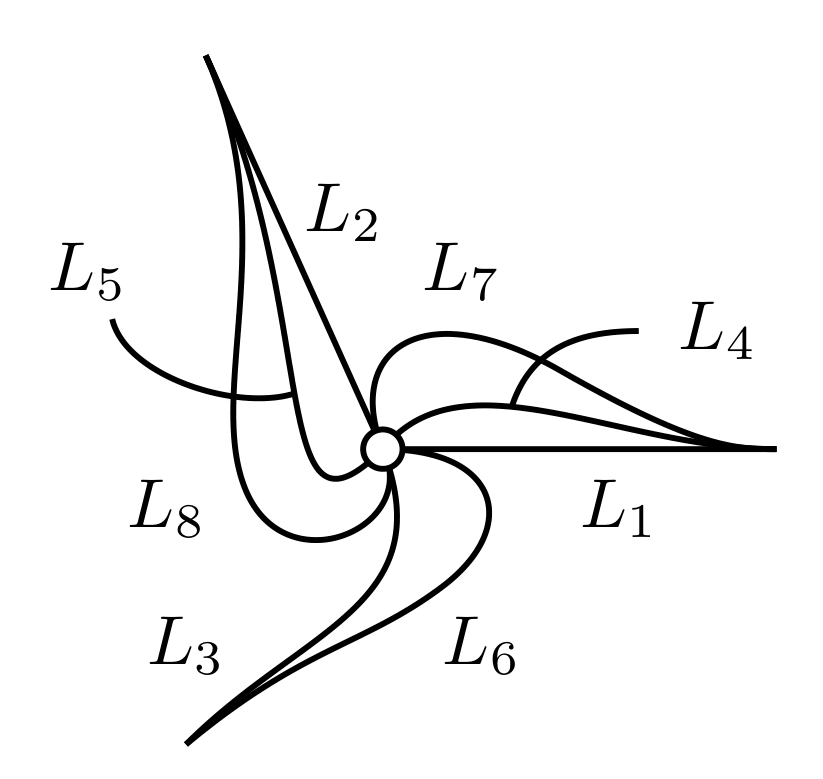
\includegraphics[width=0.31\textwidth]{figures/fig17.3.png}
  \figtitle{17.3}{$(a,b)=(1,1)$}
\end{figure}

% [Tutor Note: 原文図 17.2、17.3 的图注亦印作 (a,b)=(1,1)，而 p028 正文称三图分别对应 (a,b)=(1,1),(2,2),(3,5)；图注疑为原文误植，此处照图注原样保留。]

\section{半正交分解}

三角范畴 $\cT$ 的全子范畴 $\cN$ 称为右可容许的（right admissible），是指嵌入函子 $i\colon\cN\hookrightarrow\cT$ 具有右伴随函子 $i^{!}\colon\cT\to\cN$。同样地，当嵌入函子具有左伴随函子 $i^{*}\colon\cT\to\cN$ 时，称为左可容许的（left admissible）。$\cN$ 为右可容许的充要条件是：对任意 $X\in\cT$，存在正合三角 $N\to X\to M$，使得 $N\in\cN$ 且 $M\in\cN^{\perp}$。当 $\cT$ 与 $\cN$ 具有 Serre 函子时，

\begin{align}
  \Hom_{\cT}(X,i(N)) &\cong \Hom_{\cT}(i(N),S_{\cT}(X))^{\vee} \tag{18.1}\\
  &\cong \Hom_{\cN}(N,i^{!}\circ S_{\cT}(X))^{\vee} \tag{18.2}\\
  &\cong \Hom_{\cN}(i^{!}\circ S_{\cT}(X),S_{\cN}(N)) \tag{18.3}\\
  &\cong \Hom_{\cN}(S_{\cN}^{-1}\circ i^{!}\circ S_{\cT}(X),N) \tag{18.4}
\end{align}

由此

\begin{equation}
  i^{*} \cong S_{\cN}^{-1}\circ i^{!}\circ S_{\cT} \tag{18.5}
\end{equation}

从而左右可容许性等价。双侧可容许子范畴简称为可容许子范畴（admissible subcategory）。当存在可容许子范畴的序列 $(\cN_1,\dots,\cN_n)$ 与左可容许子范畴的递增序列 $\cT_1=\cN_1\subset\cT_2\subset\dots\subset\cT_n=\cT$，且对任意 $i=1,\dots,n-1$，$\cN_i$ 在 $\cT_i$ 中与 $\cT_{i-1}$ 左正交时，

\begin{equation}
  \cT = \langle \cN_1,\dots,\cN_n \rangle \tag{18.6}
\end{equation}

并称 $\cT=\langle\cN_1,\dots,\cN_n\rangle$ 为 $\cT$ 的半正交分解（semiorthogonal decomposition）。

三角范畴的对象 $E$ 若满足

\begin{equation}
  \Hom^{i}(E,E) =
  \begin{cases}
    \C\cdot\id_{E} & i=0,\\
    0 & \text{otherwise}
  \end{cases} \tag{18.7}
\end{equation}

则称为例外对象（exceptional object）。若例外对象的序列 $(E_1,\dots,E_n)$ 对任意 $i>j$ 与 $k\in\Z$ 满足

\begin{equation}
  \Hom^{k}(E_i,E_j) = 0 \tag{18.8}
\end{equation}

则称为例外序列（exceptional sequence）。由例外序列作为三角范畴生成的子范畴必定是可容许的。当例外序列生成 $\cT$（作为三角范畴）时，称为完备的（full）。对完备例外序列 $(E_1,\dots,E_n)$，设 $E_i$ 生成的 $\cT$ 的三角子范畴为 $\cN_i$，则存在 $\cT$ 的半正交分解 $\cT=\langle\cN_1,\dots,\cN_n\rangle$，并记作 $\cT=\langle E_1,\dots,E_n\rangle$。此时 $\cT_i$ 是由 $E_1,\dots,E_i$ 生成的 $\cT$ 的三角子范畴。

给定微分分次范畴 $\cD$ 及其上对象的序列 $(E_1,\dots,E_n)$ 时，以这些对象为对象的新微分分次范畴 $\cD^{\to}$ 定义为

\begin{equation}
  \hom_{\cD^{\to}}(E_i,E_j) :=
  \begin{cases}
    \C\cdot\id_{E_i} & i=j,\\
    \hom_{\cD}(E_i,E_j) & i<j,\\
    0 & \text{otherwise}
  \end{cases} \tag{18.9}
\end{equation}

并称之为关于 $(E_1,\dots,E_n)$ 的 $\cD$ 的有向子范畴（directed subcategory）。有向子范畴是非全子范畴的重要例子。此外，当 $\cD$ 是 Calabi–Yau 范畴（即在 $\mathrm{Ho}\,\cD$ 中 Serre 函子为整数平移的范畴），且 $(E_1,\dots,E_n)$ 通过映射锥与直和因子生成 $\cD$ 时，存在与取有向子范畴相逆的操作，称为 Calabi–Yau 扩张（Calabi–Yau extension）。这是从类似于 Fano 流形的相干层的导出范畴的范畴出发，构造类似于 Calabi–Yau 流形的相干层的导出范畴的范畴的操作。Calabi–Yau 扩张有平凡的情形 [Seg08, Bal] 与非平凡的情形 [Kel11]。例如，当 $\cD^{\to}$ 是 $\PP^{2}$ 的相干层的导出范畴、且 $(E_1,E_2,E_3)=(\cP_{\PP^{2}},\cP_{\PP^{2}}(1),\cP_{\PP^{2}}(2))$ 时，作为 $\cD^{\to}$ 的 1 维非平凡 Calabi–Yau 扩张可得椭圆曲线的相干层的导出范畴，作为 3 维平凡的 Calabi–Yau 扩张可得 $\PP^{2}$ 的典范丛的全空间的相干层的导出范畴。

% [Tutor Note: 原文此处作花体 𝒫_{P²}（即 \cP_{\PP^{2}}），按 Beilinson 例外列通常应为 𝒪_{P²}；此处照录原文，请审校确认。]

有向子范畴的导出范畴按定义具有完备例外序列，Fukaya–Seidel 范畴正是其例。由同调镜像对称，这与 [Kaw06b] 关于完备环面流形的相干层的导出范畴具有完备例外序列的结果相对应。此外，去掉若干例外对象即可得到可容许子范畴，人们期待这与极小模型理论中的收缩、flop 相对应 [Kaw13, BFK, BO, BO02, Kuzb]。[AKO08] 利用这一点证明了 Hirzebruch 曲面的同调镜像猜想。另外，[Ker08] 考察了对应于环面曲面的加权爆破的镜像的行为。

对于半正交分解

\begin{equation}
  \cT = \langle \cN_1,\cN_2 \rangle \tag{18.10}
\end{equation}

称 $\phi = i_2^{*}\circ i_1\colon\cN_1\to\cN_2$ 为粘贴函子（gluing functor）。例如，设 $\PP^{2}$ 的单点爆破为 $\pi\colon X\to\PP^{2}$，则 $X$ 的相干层的导出范畴具有

\begin{equation}
  D^{b}\,\mathrm{coh}\,X = \bigl\langle \cO_E(-1),\,\pi^{*}D^{b}\,\mathrm{coh}\,\PP^{2}\bigr\rangle,
  \qquad
  \pi^{*}D^{b}\,\mathrm{coh}\,\PP^{2} = \langle \cO,\cO(H),\cO(2H) \rangle \tag{18.11}
\end{equation}

这样的半正交分解 [Orl92]。此时

\begin{equation}
  M := \phi(\cO_E(-1)) = i_2^{*}(\cO_E(-1)) \in {}^{\perp}\bigl(\pi^{*}D^{b}\,\mathrm{coh}\,\PP^{2}\bigr) \tag{18.12}
\end{equation}

而 $M$ 由 $N\in\pi^{*}D^{b}\,\mathrm{coh}\,\PP^{2}$ 通过正合三角

\begin{equation}
  M \to \cO_E(-1) \to N \tag{18.13}
\end{equation}

所刻画。这是沿 (18.11) 对 $\cO_E(-1)$ 作变位所得的

\begin{equation}
  D^{b}\,\mathrm{coh}\,X = \bigl\langle \pi^{*}D^{b}\,\mathrm{coh}\,\PP^{2},\,M\bigr\rangle \tag{18.14}
\end{equation}

由变位与 Serre 函子的关系，

\begin{equation}
  M[2] \cong \cO_E(-1)\otimes\omega_X^{-1} \cong \cO_E(E)\otimes\cO(3H-E) \cong \cO_E(3H) \cong \cO_E \tag{18.15}
\end{equation}

而 $N$ 是对应于

\begin{align}
  \Hom(\cO_E[-2],\cO_E(-1)) &\cong \Ext^{2}(\cO_E,\cO_E(-1)) \tag{18.16}\\
  &\cong \Ext^{2}\bigl(\{\cO(-E)\to\cO\},\cO_E(-1)\bigr) \tag{18.17}\\
  &\cong \mathbb{H}^{2}\bigl(\{\cO_E(-1)\to\cO_E(-2)\}\bigr) \tag{18.18}\\
  &\cong \C \tag{18.19}
\end{align}

的生成元的映射锥。具体写出变位，则由

\begin{equation}
  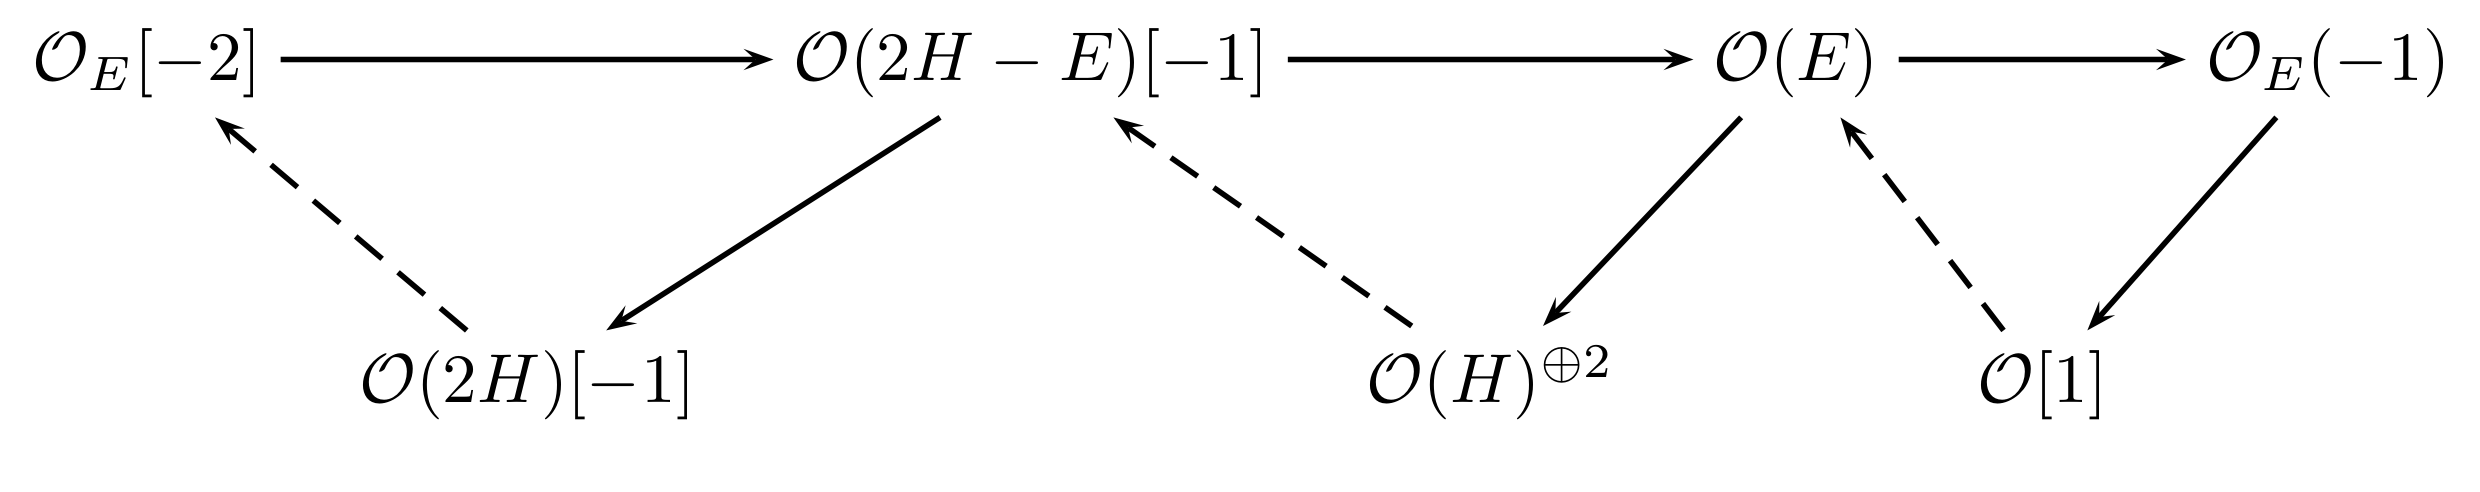
\includegraphics[width=0.82\textwidth]{figures/eq18.20.png}
  \tag{18.20}
\end{equation}

% [Tutor Note: (18.20) 为含虚线斜箭头的图表，preamble 未加载 tikz/tikz-cd，故按页面裁图原样嵌入（work/figures/eq18.20.png）；实线与虚线箭头、上下位置均照原文。]

得到

\begin{equation}
  N \cong \bigl\{\cO_E[-2]\to\cO_E(-1)\to\pi^{*}\cO_p[1]\bigr\} \cong \pi^{*}\cO_p[1] \tag{18.21}
\end{equation}

其中

\begin{equation}
  \cO_p \cong \bigl\{\cO(2H)\to\cO(H)^{\oplus 2}\to\cO\bigr\} \tag{18.22}
\end{equation}

是爆破中心 $p\in\PP^{2}$ 的结构层。

由相干层的导出范畴的半正交分解得到的 Hochschild 上同调正合列

\begin{equation}
  \dots \to \mathrm{HH}^{i}(\cA) \to \mathrm{HH}^{i}(\cA_1)\oplus\mathrm{HH}^{i}(\cA_2) \to \Ext(\phi,\phi) \to \dots \tag{18.23}
\end{equation}

由 [Kuza] 给出。此外，相关结果亦见于 [Han14]。

根据森田理论，Abel 范畴之间的函子 $\phi\colon\mathrm{mod}\,A_1\to\mathrm{mod}\,A_2$ 由 $(A_1,A_2)$ 双模 $M$（左 $A_1$、右 $A_2$）表示为 $X_1\mapsto X_1\otimes_{A_1}M$。在集合

\begin{equation}
  \begin{pmatrix} A_2 & \\ M & A_1 \end{pmatrix}
  := \left\{\,
  \begin{pmatrix} a_2 & 0\\ m & a_1 \end{pmatrix}
  \;\middle|\;
  a_1\in A_1,\ a_2\in A_2,\ m\in M
  \,\right\} \tag{18.24}
\end{equation}

上以

\begin{equation}
  \begin{pmatrix} a_2 & 0\\ m & a_1 \end{pmatrix}
  \cdot
  \begin{pmatrix} a_2' & 0\\ m' & a_1' \end{pmatrix}
  =
  \begin{pmatrix} a_2a_2' & 0\\ m a_2 + a_1 m' & a_1a_1' \end{pmatrix} \tag{18.25}
\end{equation}

定义乘法，所得对象记作 $T(A_1,A_2,M)$，称为三角矩阵代数（triangular matrix algebra）。

\begin{equation}
  \left(
  \begin{pmatrix} u_2 & u_1 \end{pmatrix}
  \begin{pmatrix} a_2 & \\ m & a_1 \end{pmatrix}
  \right)
  \begin{pmatrix} a_2' & \\ m' & a_1' \end{pmatrix}
  =
  \Bigl(
  (u_2a_2)a_2' + (u_1m)a_2' + (u_1a_1)m'
  \quad
  (u_1a_1)a_1'
  \Bigr), \tag{18.26}
\end{equation}

\begin{equation}
  \begin{pmatrix} u_2 & u_1 \end{pmatrix}
  \left(
  \begin{pmatrix} a_2 & \\ m & a_1 \end{pmatrix}
  \begin{pmatrix} a_2' & \\ m' & a_1' \end{pmatrix}
  \right)
  =
  \Bigl(
  u_2(a_2a_2') + u_1(ma_2') + u_1(a_1m')
  \quad
  u_1(a_1a_1')
  \Bigr) \tag{18.27}
\end{equation}

因此，给出 $T(A_1,A_2,M)$-模等价于给出三元组 $(U_1,U_2,\varphi)$：$U_1$ 为 $A_1$-模，$U_2$ 为 $A_2$-模，$\varphi\colon U_1\otimes_{A_1}M\to U_2$ 为 $A_2$-模同态。三元组 $(U_1,U_2,\varphi)$ 与 $(U_1',U_2',\varphi')$ 之间的态射由组 $\psi=(\psi_1,\psi_2)$（其中 $\psi_1\in\Hom_{A_1}(U_1,U_1')$、$\psi_2\in\Hom_{A_2}(U_2,U_2')$）给出，其要求是图表

\begin{equation}
  \begin{array}{c@{\quad}c@{\quad}c}
    U_1\otimes_{A_1}M & \xrightarrow{\ \ \varphi\ \ } & U_2\\[2.6ex]
    \psi_1\otimes\id_M\Big\downarrow & & \Big\downarrow\psi_2\\[2.6ex]
    U_1'\otimes_{A_1}M & \xrightarrow{\ \ \varphi\ \ } & U_2'
  \end{array} \tag{18.28}
\end{equation}

交换。

定义函子 $i_1\colon\mathrm{mod}\,A_1\to\mathrm{mod}\,T(A_1,A_2,M)$ 与 $i_2\colon\mathrm{mod}\,A_2\to\mathrm{mod}\,T(A_1,A_2,M)$ 为

\begin{equation}
  i_1(U_1) = (U_1,0,0),\quad
  i_2(U_2) = (\Hom_{A_2}(M,U_2),U_2),\mathrm{ev}) \tag{18.29}
\end{equation}

则

\begin{align}
  \Hom_{A_2}(\phi(U_1),U_2) &:= \Hom_{A}(i_1(U_1),i_2(U_2)) \tag{18.30}\\
  &\cong \Hom_{A_1}\bigl(U_1,\Hom_{A_2}(M,U_2)\bigr) \tag{18.31}\\
  &\cong \Hom_{A_2}(U_1\otimes_{A_1}M,U_2), \tag{18.32}\\
  \Hom_{A}(i_1(U_1),i_2(U_2)) &= 0 \tag{18.33}
\end{align}

% [Tutor Note: (18.29) 原文的括号作 i_2(U_2)=(\Hom_{A_2}(M,U_2),U_2),\mathrm{ev})，右括号多出一个；按原文照录，疑应为三元组 (\Hom_{A_2}(M,U_2),U_2,\mathrm{ev})。]

在三角矩阵代数中，当 $A_1=\C$ 时，称

\begin{equation}
  A = T(\C,A_2,M) = \begin{pmatrix} A_2 & \\ M & \C \end{pmatrix} \tag{18.34}
\end{equation}

为 $A_2$ 的一点余扩张（one-point coextension）。此外，对于左 $A_2$-模 $N$，称

\begin{equation}
  \begin{pmatrix} A_2 & N\\ & \C \end{pmatrix} \tag{18.35}
\end{equation}

为 $A_2$ 关于 $N$ 的一点扩张（one-point extension）。这些概念由 [Rin84] 引入。

作为构造三角矩阵代数的方法，有对幂等列取有向子代数的做法。若代数 $A$ 的元素列 $(e_1,e_2)$ 满足

\begin{equation}
  e_1^{2} = e_1,\quad e_2^{2} = e_2,\quad e_1e_2 = e_2e_1 = 0,\quad 1 = e_1+e_2, \tag{18.36}
\end{equation}

则称之为 $A$ 的幂等列。对代数 $A$ 的任意幂等元 $e$，$(e,1-e)$ 是幂等列。对幂等列 $(e_1,e_2)$，置

\begin{equation}
  A_1 := e_1Ae_1,\quad A_2 := e_2Ae_2,\quad M := e_1Ae_2,\quad N := e_2Ae_1 \tag{18.37}
\end{equation}

则 $M$ 是 $(A_1,A_2)$ 双模、$N$ 是 $(A_2,A_1)$ 双模，且 $A$ 分解为

\begin{equation}
  A = \begin{pmatrix} A_1 & N\\ M & A_2 \end{pmatrix} \tag{18.38}
\end{equation}

此时置

\begin{equation}
  A^{\to} := T(A_1,A_2,M) \tag{18.39}
\end{equation}

称之为与幂等列 $(e_1,e_2)$ 相伴的 $A$ 的有向子代数（directed subalgebra）。

三角矩阵代数与 Abel 范畴及导出范畴中的 recollement（再粘合）概念密切相关。这是源自 [BBD82] 的概念，关于它可参见例如 [FP04]。

三角矩阵代数的 Hochschild 上同调具有长正合列 [Cib00, GG, MP00, GS02, GMS03]：

\begin{equation}
  \dots \to \mathrm{HH}^{i}(A) \to \mathrm{HH}^{i}(A_1)\oplus\mathrm{HH}^{i}(A_2)
  \to \Ext_{A_1^{\mathrm{op}}\otimes A_2}(M,M) \to \dots \tag{18.40}
\end{equation}

在一点扩张的情形，这些结果更早即已由 [Hap89] 给出。

% CHUNK c08 DONE pages p029–p032

% =====================================================================
%  chunk c09 —— 植田一石《ホモロジー的ミラー対称性》
%  第 19–24 节，原书 p033–p036
%  编号公式 34 条（p033: 7，p034: 8，p035: 9，p036: 10），逐页据 pages/pNNN.png 抄录
% =====================================================================
% [Tutor Note: 关于本 chunk 的公式条数。work/BRIEF.md 对 c09 记「50 条编号公式」，
%  但按页面图像逐页核对，p033–p036 上实际印出的编号公式共 34 条。BRIEF 的 50 应来自
%  work/tags_bypage.txt 的原始命中数（10+12+16+12=50），其中包含正文中的公式交叉引用
%  （如 p033 上的 (2.5) 出现 3 次、(21.1)/(21.2) 在 p034 正文中反复被引用、p035 上的
%  (21.6)、p036 上的 (23.1) 等）以及跨页重复计数，并非编号公式的条数。此处按图像
%  一一对应抄录 34 条，未增补任何编号，请 Lead 核定 BRIEF 的计数口径。]

\section{从同调镜像猜想走向 SYZ 猜想}

假设对 Calabi--Yau 流形的对 $(M, W)$，同调镜像对称 (2.5) 成立。于是对 $W$ 的每个点 $p$，存在 $M$ 的 Fukaya 范畴中对应于 $p$ 处的点层（skyscraper sheaf）$\cO_p$ 的对象。它一般而言是拉格朗日子流形的复形，但朴素地设想，假定它由 $M$ 的单个拉格朗日子流形实现。把这个拉格朗日子流形记作 $L_p$，则由范畴等价 (2.5) 得到
\begin{equation}
\mathrm{HF}^{*}(L_p) \cong \Ext^{*}(\cO_p, \cO_p) \tag{19.1}
\end{equation}
这里 $\mathrm{HF}^{*}(L_p)$ 是 $L_p$ 的 Floer 上同调。另一方面，$n$ 维复流形上点层的上同调总是同构于 $n$ 维环面 $T^n := (S^1)^n$ 的通常上同调；
\begin{equation}
\Ext^{*}(\cO_p, \cO_p) \cong H^{*}(T^n) \tag{19.2}
\end{equation}
在适当条件下，拉格朗日子流形的 Floer 上同调与通常上同调一致，因此若宽松地考虑，可以期望 $L_p$ 是环面。对相异的两点 $p, q \in W$，由范畴等价 (2.5) 得到
\begin{equation}
\mathrm{HF}^{*}(L_p, L_q) \cong \Ext^{*}(\cO_p, \cO_q) = 0 \tag{19.3}
\end{equation}
于是再次宽松地考虑，可以期望 $L_p$ 与 $L_q$ 不相交。进而，点层的集合 $\{\cO_p\}_{p \in W}$ 是张成类（spanning class，即对任意 $p \in W$，若 $\Hom(E, \cO_p) = 0$ 则 $E \cong 0$），因此自然期望，如此得到的这些 $L_p$ 铺满 $W$ 的整体，给出 $W$ 的拉格朗日环面纤维化。不过，Fukaya 范畴中的同构类在把拉格朗日子流形沿 Hamilton 同胚移动时不变，因此需要在拉格朗日子流形的 Hamilton 同痕类中取良好的代表元。类似的问题在复几何一侧也存在，构成模空间时的稳定性（stability）正对应于此。相干层的导出范畴中的稳定性，与 Calabi--Yau 流形的 flop 有很深的关联 [Bri02]。

\section{特殊拉格朗日子流形}

作为 Kähler 流形上的相干层，除点层之外还有全纯向量丛（holomorphic vector bundle）。由 Donaldson 与 Uhlenbeck--Yau 证明的小林--Hitchin 对应（Hitchin--Kobayashi correspondence），稳定的（stable）全纯向量丛与不可约 Hermite Yang--Mills 联络（irredubicle Hermitian Yang--Mills connection）成一一对应。在镜像一侧与之对应而受到期望的，正是特殊拉格朗日子流形。

% [Tutor Note: 上句中原文英文为 “irredubicle”，疑为 “irreducible” 之误，此处照录原文，请审校确认。]

我们曾把和乐群为 $\mathrm{SU}(n)$ 的子群的 $2n$ 维黎曼流形 $(M, g)$ 称为 Calabi--Yau 流形。$\C^n$ 上的 $(1, 1)$ 形式
\begin{equation}
\omega_0 := \frac{\sqrt{-1}}{2}\left(dz_1 \wedge d\bar z_1 + \cdots + dz_n \wedge d\bar z_n\right) \tag{20.1}
\end{equation}
与 $(n, 0)$ 形式
\begin{equation}
\Omega_0 := dz_1 \wedge \cdots \wedge dz_n \tag{20.2}
\end{equation}
在 $\mathrm{SU}(n)$ 的作用下不变，因此从某点的切空间出发、通过平行移动加以延拓，便可得到 Calabi--Yau 流形上的微分形式 $\omega$ 与 $\Omega$，使其共变微分为零。它们分别给出 $M$ 的 Kähler 形式与全纯体积形式（holomorphic volume form）。$\omega_0$ 与 $\Omega_0$ 满足关系式
\begin{equation}
\frac{1}{n!}\omega_0^{n} = (-1)^{n(n-1)/2}\left(\frac{\sqrt{-1}}{2}\right)^{n}\Omega_0 \wedge \bar\Omega_0 \tag{20.3}
\end{equation}
因此 $\omega$ 与 $\Omega$ 也同样满足
\begin{equation}
\frac{1}{n!}\omega^{n} = (-1)^{n(n-1)/2}\left(\frac{\sqrt{-1}}{2}\right)^{n}\Omega \wedge \bar\Omega \tag{20.4}
\end{equation}
$M$ 的 $n$ 维子流形 $L$ 满足
\begin{equation}
\omega|_{L} = 0 \tag{20.5}
\end{equation}
时，称 $L$ 为拉格朗日子流形（Lagrangian submanifold）。若存在某个实数 $\theta$，使拉格朗日子流形 $L$ 满足
\begin{equation}
\operatorname{Im}\left(\ee^{\sqrt{-1}\theta}\Omega\right)\Big|_{L} = 0 \tag{20.6}
\end{equation}
则称 $L$ 为相位（phase）为 $\theta$ 的特殊拉格朗日子流形（special Lagrangian submanifold）。把 $\Omega$ 乘以常数即总可使相位为 $0$，因此只要处理单个特殊拉格朗日子流形，相位就不是本质的。

\section{极小子流形}

设 $(M, g_M)$ 为黎曼流形，$L$ 为其子流形。$L$ 的切丛关于 $g_M$ 的正交补空间称为 $L$ 的法丛（normal bundle），记作 $N_{L/M}$；
\begin{equation}
TM_{L} := TL \perp N_{L/M}. \tag{21.1}
\end{equation}
对 $L$ 上的向量场 $v, w \in \Gamma(TL)$，任意取 $M$ 上的向量场 $\tilde v, \tilde w \in \Gamma(TM)$ 使 $\tilde v|_{L} = v$ 且 $\tilde w|_{L} = w$，并置
\begin{equation}
B(v, w) := \pi_{N_{L/M}}\left(\nabla_{\tilde v}\tilde w\right) \tag{21.2}
\end{equation}
其中，
\begin{equation}
\pi_{N_{L/M}} : TM_{L} \to N_{L/M} \tag{21.3}
\end{equation}
是关于正交分解 (21.1) 的投影，$\nabla$ 是 $TM$ 关于 $g_M$ 的 Levi-Civita 联络。(21.2) 的右端显然不依赖于 $\tilde v$ 的取法。又，由 $\tilde v|_{L}, \tilde w|_{L} \in \Gamma(TM|_{L})$ 是 $\Gamma(TL)$ 的元素可知 $[\tilde v, \tilde w]|_{L} \in \Gamma(TM|_{L})$ 也是 $\Gamma(TL)$ 的元素，再由 Levi-Civita 联络的零挠率条件 $\nabla_{\tilde v}\tilde w - \nabla_{\tilde w}\tilde v = [\tilde v, \tilde w]$，可知 (21.2) 的右端关于 $\tilde v$ 与 $\tilde w$ 的交换是对称的。因此 (21.2) 的右端也不依赖于 $\tilde w$ 的取法，它确定 $\Gamma(\mathrm{Sym}^{2}\,T^{*}L \otimes N_{L/M})$ 的一个元素，称之为 $L$ 的第二基本形式（second fundamental form）。关于 $L$ 的度量 $g_L := g|_{L}$ 的第二基本形式 $B$ 的迹（trace），称为 $L$ 的平均曲率（mean curvature）；
\begin{equation}
H := \operatorname{tr}_{g|_{L}} B \in C^{\infty}(L, N_{L_M}). \tag{21.4}
\end{equation}
关于体积泛函
\begin{equation}
\operatorname{Vol}(L) := \int_{L}\operatorname{vol}L \tag{21.5}
\end{equation}
的 Euler--Lagrange 方程，已知给出二阶非线性偏微分方程
\begin{equation}
H = 0 \tag{21.6}
\end{equation}

% [Tutor Note: (21.4) 中 $C^\infty$ 的第二个变量原文印作 $N_{L_M}$（M 为 L 的下标），
%  与 (21.2)(21.3) 的 $N_{L/M}$ 不一致，疑为排版时漏掉斜线；此处照录图像，请审校确认。]

\section{校准几何}

黎曼流形 $(M, g_M)$ 上的 $k$ 次微分形式若满足以下两个条件，则称为 $k$ 次校准形式（calibration）：
\begin{enumerate}[label=\arabic*.]
\item $\varphi$ 是闭形式。
\item 对任意点 $p \in M$ 与任意有向的 $k$ 维子空间 $W \subset T_pM$，不等式
\begin{equation}
\varphi\big|_{\wedge^{k}W} \le \operatorname{vol}W \tag{22.1}
\end{equation}
成立。
\end{enumerate}
若 $M$ 的有向 $k$ 维子流形 $N$ 对任意 $p \in N$ 都满足不等式 (22.1) 中的等号
\begin{equation}
\varphi\big|_{\wedge^{k}T_pN} = \operatorname{vol}_{T_pN} \tag{22.2}
\end{equation}
则称 $N$ 为校准子流形（calibrated submanifold）。由校准形式的定义立即可得不等式
\begin{equation}
\operatorname{Vol}(N, g|_{N}) = \int_{N}\operatorname{vol}_{N} \le \int_{N}\varphi \tag{22.3}
\end{equation}
注意，(22.3) 的右端只依赖于 $N$ 的同调类 $[N] \in H_k(M, \Z)$。这是关于 Yang--Mills--Higgs 泛函的 Bogomolnyi--Prasad--Sommerfield 不等式的类似物。由不等式 (22.3) 立即推出，校准子流形在其所属的同调类中具有最小体积。特别地，校准子流形是极小子流形。极小子流形的方程 (21.6) 与校准子流形的方程 (22.2) 之间的关系，与 Yang--Mills 方程 $D^{*}F = 0$ 和 ASD 方程 $*F = -F$ 之间的关系十分相似。前者是二阶偏微分方程，给出泛函的驻点；后者是一阶偏微分方程，给出泛函的最小值。

校准形式与校准子流形的概念是由 [HL82] 引入的。校准形式最基本的例子是 Kähler 流形中 Kähler 形式的幂 $\omega^{k}$；此时成为校准子流形的充要条件是：它是复子流形。对 Calabi--Yau 流形 $(M, g, J, \omega, \Omega)$，$\operatorname{Re}\Omega$ 是校准形式，此时的校准子流形是特殊拉格朗日子流形。其他校准子流形的例子，还有 $G_2$ 流形中的结合子流形（associative 3-fold）、余结合子流形（coassociative 4-fold），以及 $\mathrm{Spin}(7)$ 流形中的 Cayley 子流形（Caley 4-fold）等。

% [Tutor Note: 原文 “Caley 4-fold” 疑为 “Cayley 4-fold” 之误，此处照录原文，请审校确认。]

\section{McLean 定理}

设 $(M, g_M, J, \omega, \Omega)$ 为 Calabi--Yau 流形，$L$ 为其特殊拉格朗日子流形。关于 $L$ 的黎曼度量 $g_L := (g_M)|_{L}$ 的 Hodge 星算子记作 $*_{L} : \Omega^{k}(L) \to \Omega^{n-k}(L)$。设 $\nu \in \Gamma(N_{L/X})$ 为 $L$ 的法向量场，则
\begin{equation}
(\iota_{\nu}\operatorname{Im}\Omega)\big|_{L} = -*_{L}\left((\iota_{\nu}\omega)\big|_{L}\right) \tag{23.1}
\end{equation}
成立。事实上，(23.1) 不含微分，因此逐点取切空间的适当基，即可归结为 $M = \C^{n}$ 且 $L = \R^{n}$、并且
\begin{align}
\Omega &= dz_1 \wedge \cdots \wedge dz_n = (dx_1 + \sqrt{-1}dy_1) \wedge \cdots \wedge (dx_n + \sqrt{-1}dy_n), \tag{23.2}\\
\omega &= dx_1 \wedge dy_1 + \cdots + dx_n \wedge dy_n, \tag{23.3}\\
\nu &= \frac{\partial}{\partial y_1} \tag{23.4}
\end{align}
的情形；此时容易看出 (23.1) 的两端都是 $dx_2 \wedge \cdots \wedge dx_n$。

$L$ 沿法向量场 $\nu$ 的微小变形成为特殊拉格朗日子流形的充要条件是
\begin{equation}
\cL_{\nu}\operatorname{Im}\Omega = \cL_{\nu}\omega = 0 \tag{23.5}
\end{equation}
利用 Cartan 的同伦公式
\begin{equation}
\cL_{\nu} = d \circ \iota_{\nu} + \iota_{\nu}d \tag{23.6}
\end{equation}
以及 $\Omega$ 和 $\omega$ 是闭形式这一点，此条件可改写为
\begin{equation}
d\iota_{\nu}\omega = d\iota_{\nu}\operatorname{Im}\Omega = 0 \tag{23.7}
\end{equation}
由 (23.1)，此条件又等价于
\begin{equation}
d\iota_{\nu}\omega = d(*\iota_{\nu}\omega) = 0, \tag{23.8}
\end{equation}
即 $\iota_{\nu}\omega$ 是调和 $1$ 形式。通过使用 Banach 流形上的隐函数定理，McLean 证明了下面的定理：

\begin{theorem}[{[McL98, Theorem 3.6]}]
特殊拉格朗日子流形的模空间是光滑的，且其在 $L$ 处的切空间自然同构于 $L$ 上的调和形式空间。
\end{theorem}

特别地，特殊拉格朗日子流形的模空间的维数等于 $L$ 的第一 Betti 数。对 $\nu_1, \nu_2 \in \Gamma(N_{L/M})$，置
\begin{equation}
g(\nu_1, \nu_2) = \int_{L_b}(\iota_{\nu_1}\omega) \wedge *(\iota_{\nu_2}\omega) \tag{23.9}
\end{equation}
则它给出特殊拉格朗日子流形的模空间的度量，称之为 McLean 度量（McLean metric）。

% [Tutor Note: (23.1) 上方的 ν ∈ Γ(N_{L/X}) 中原文用 X，与后文 Γ(N_{L/M}) 不一致，
%  疑为 M 之误；此处照录图像。(23.9) 的积分区域原文印作 L_b（b 为下标），
%  疑为 L 之误或排印残留；此处照录图像。]

\section{Hessian 结构}

仿射流形 $M$ 上的黎曼度量 $g$ 称为 Hessian 度量（Hessian metric），是指：对每点 $p \in M$，存在 $p$ 的邻域 $U$ 的仿射坐标 $\{y_i\}_{i=1}^{n}$ 与 $U$ 上的函数 $K$，使得
\begin{equation}
g_{ij} = \frac{\partial^{2}K}{\partial y_i\partial y_j} \tag{24.1}
\end{equation}
成立。用确定 $M$ 的仿射结构的联络 $D$，(24.1) 可写成不依赖坐标的形式
\begin{equation}
g = DdK \tag{24.2}
\end{equation}
注意，一般地 $D$ 与 $g$ 的 Levi-Civita 联络 $\nabla$ 并不一致。由于度量 $g$ 正定，$K$ 成为凸函数，并且除加仿射函数的自由度外被唯一确定。

用仿射坐标把 $U$ 与 $\R^{n}$ 的开集等同，并定义映射 $\check y = (\check y_1, \dots, \check y_n) : U \to \R^{n}$ 为
\begin{equation}
\check y_i = \frac{\partial K}{\partial y_i} \tag{24.3}
\end{equation}
则由 $K$ 的凸性，$\check y$ 是单射，并给出 $U$ 的坐标。进而，定义 $U$ 上的函数 $\check K$ 为
\begin{equation}
\check K := \sum_{i=1}^{n}\check y_i y_i - K \tag{24.4}
\end{equation}
则
\begin{align}
\frac{\partial\check K}{\partial\check y_i} &= y_i + \sum_{j=1}^{n}\check y_j\frac{\partial y_j}{\partial\check y_i} - \frac{\partial K}{\partial\check y_i} \tag{24.5}\\
&= y_i + \sum_{j=1}^{n}\frac{\partial K}{\partial y_j}\frac{\partial y_j}{\partial\check y_i} - \frac{\partial K}{\partial\check y_i} \tag{24.6}\\
&= y_i \tag{24.7}
\end{align}

% 第 24 节正文续 p037，由 c10 接续。

% CHUNK c09 DONE pages p033–p036

% =====================================================================
%  c10 —— 第 25–30 节（p037–p042）
%  节标题起始页：25→p037，26→p037，27→p038，28→p039，29→p040，30→p040
%  编号公式（按页面图像实际条数）：63 条
% =====================================================================

% [Tutor Note: 原文 p036 末尾为公式 (24.7)，p037 顶端以接续词「かつ」开头、后接公式 (24.8)–(24.13)，句末「となる」在本页；此处按跨页断句处理，正文从此处直接接续第 24 节。]
且
\begin{align}
  g\left(\frac{\partial}{\partial \tilde y_i}, \frac{\partial}{\partial \tilde y_j}\right)
  &= g\left(\sum_{k=1}^{n}\frac{\partial y_k}{\partial \tilde y_i}\frac{\partial}{\partial y_k},
    \sum_{l=1}^{n}\frac{\partial y_l}{\partial \tilde y_i}\frac{\partial}{\partial y_l}\right) \tag{24.8}\\
  &= \sum_{k,l=1}^{n}\frac{\partial y_k}{\partial \tilde y_i}\frac{\partial y_l}{\partial \tilde y_i}
    g\left(\frac{\partial}{\partial y_k}, \frac{\partial}{\partial y_l}\right) \tag{24.9}\\
  &= \sum_{k,l=1}^{n}\frac{\partial y_k}{\partial \tilde y_i}\frac{\partial y_l}{\partial \tilde y_i}
    \frac{\partial \tilde y_k}{\partial y_l} \tag{24.10}\\
  &= \sum_{k=1}^{n}\frac{\partial y_k}{\partial \tilde y_i}\frac{\partial y_k}{\partial \tilde y_j} \tag{24.11}\\
  &= \sum_{k=1}^{n}\frac{\partial y_j}{\partial \tilde y_i} \tag{24.12}\\
  &= \frac{\partial^2 \tilde K}{\partial \tilde y_i\partial \tilde y_j} \tag{24.13}
\end{align}
成立。从而，$(U,g)$ 以 $((\tilde y_i)_{i=1}^{n})$ 为仿射坐标而具有 Hessian 结构；这称为对偶 Hessian 结构（dual Hesse structure）。又，从 $((y_i)_{i=1}^{n},K)$ 到 $((\tilde y_i)_{i=1}^{n},\tilde K)$ 的变换称为 Legendre 变换（Legendre transformation）。这一构造经粘合给出 $M$ 的对偶 Hessian 结构。

% [Tutor Note: 原文 (24.8)–(24.10) 第二个求和因子中偏导的下标均印作 \tilde y_i（按推导似应为 \tilde y_j）；又 (24.12) 印作 \sum_{k=1}^{n}\partial y_j/\partial\tilde y_i，求和指标 k 未在项中出现。以上均按图像照录，请审校。]

\section{辛仿射结构}

设 $\pi: X \to B$ 为 Lagrange 环面纤维丛。对底空间中的点 $b_0$，取其邻域 $U$ 上 $\pi$ 的平凡化 $\pi^{-1}(U) \cong U\times T^n$。令 $\{\gamma_1,\dots,\gamma_n\}$ 为环面 $T^n := \R^n/\Z^n$ 上 1-闭链的标准基，作为 $\omega$ 沿 $\gamma_i$ 的积分而定义
\begin{equation}
  \omega_i := \int_{\gamma_i}\omega \tag{25.1}
\end{equation}
这是对 $\nu \in T_bB$ 给出
\begin{equation}
  \omega_i(\nu) := \int_{\gamma_i}\iota_{\tilde\nu}(\omega) \tag{25.2}
\end{equation}
的底空间上的 1 次微分形式。其中，$\tilde\nu$ 是 $TX|_{L_b}$ 的截面，使得对任意 $x \in L_b := \pi^{-1}(b)$ 有 $\pi_*(\tilde\nu(x)) = \nu$。由 $L_b$ 的 Lagrange 条件
\begin{equation}
  \omega|_{L_b} = 0 \tag{25.3}
\end{equation}
可知 (25.2) 的右端不依赖 $\tilde\nu$ 的取法而确定。又，由 $\omega$ 是闭形式可知 $\omega_i$ 也是闭形式。从而，若 $U$ 取得足够小，则存在 $U$ 上的函数 $y_i$ 满足
\begin{equation}
  \dd y_i = \omega_i \tag{25.4}
\end{equation}
这样的 $y_i$ 在相差热带仿射变换 $\mathrm{GL}_n(\Z)\ltimes\R^n$ 的作用的意义下唯一确定。在 $U\cap U'$ 上，函数 $\{y_i\}_{i=1}^{n}$ 与 $\{y'_i\}_{i=1}^{n}$ 通过 $\mathrm{GL}_n(\Z)\ltimes\R^n$ 的作用互相联系。由此在 $B$ 上确定热带仿射结构，称之为 $B$ 的辛仿射结构（symplectic affine strcutre）。

% [Tutor Note: 原文英文括注印作 “strcutre”（structure 之误），此处照录；下文 (26.2) 后的 “complex tropical affine strcutre” 同。]

\section{复仿射结构}

同样，令 $\{\Gamma_1,\dots,\Gamma_n\}$ 为 $T^n$ 的 $(n-1)$-闭链的标准基。
\begin{equation}
  \lambda_i = -\int_{\Gamma_i}\Im\Omega \tag{26.1}
\end{equation}
如此设定，则 $\dd\lambda_i = 0$，于是存在 $\{\tilde y_i\}_{i=1}^{n}$ 使得
\begin{equation}
  \lambda_i = \dd\tilde y_i \tag{26.2}
\end{equation}
成立。$B$ 上由此确定以该 $\{\tilde y_i\}_{i=1}^{n}$ 为局部坐标的热带仿射结构，称之为 $B$ 的复仿射结构（complex tropical affine strcutre）。

\section{Hitchin 定理}

\begin{theorem}
McLean 度量是 Hessian 度量，且辛仿射结构与复仿射结构互为对偶。
\end{theorem}

\begin{proof}
选取 $\{\gamma_i\}_{i=1}^{n}$ 与 $\{\Gamma_i\}_{i=1}^{n}$ 使得 $\gamma_i\cdot\gamma_j = \delta_{ij}$。
\begin{equation}
  \delta_{ij} = \dd y_i\left(\frac{\partial}{\partial y_j}\right)
  = \omega_i\left(\frac{\partial}{\partial y_j}\right)
  = \int_{\gamma_i}\iota_{\frac{\partial}{\partial y_j}}\omega \tag{27.1}
\end{equation}
所以，
\begin{equation}
  \left[\iota_{\frac{\partial}{\partial y_j}}\omega\right] \in H^1(L_b) \tag{27.2}
\end{equation}
是与 $\gamma_j$ 对偶的元 $\gamma_j^*$。
\begin{align}
  g_{ij} &:= g\left(\frac{\partial}{\partial y_i}, \frac{\partial}{\partial y_j}\right) \tag{27.3}\\
  &= -\int_{L_b}\left(\iota_{\frac{\partial}{\partial y_i}}\omega\right)
    \wedge\left(\iota_{\frac{\partial}{\partial y_j}}\Im\Omega\right) \tag{27.4}\\
  &= -\int_{L_b}\gamma_i^*\wedge\left(\iota_{\frac{\partial}{\partial y_j}}\Im\Omega\right) \tag{27.5}\\
  &= -\int_{\Gamma_i}\iota_{\frac{\partial}{\partial y_j}}\Im\Omega \tag{27.6}\\
  &= \frac{\partial \tilde y_i}{\partial y_j} \tag{27.7}
\end{align}
成立，而 $g_{ij} = g_{ji}$，故
\begin{equation}
  \frac{\partial \tilde y_i}{\partial y_j} = \frac{\partial \tilde y_j}{\partial y_i} \tag{27.8}
\end{equation}
从而存在某个 $K$ 使得
\begin{equation}
  \tilde y_i = \frac{\partial K}{\partial y_i} \tag{27.9}
\end{equation}
可以这样写。这表明 $g$ 是 Hessian 度量、$(y_i)_{i=1}^{n}$ 与 $(\tilde y_i)_{i=1}^{n}$ 是 Legendre 对偶的仿射坐标。
\end{proof}

% [Tutor Note: (27.1) 前的条件原文印作 \gamma_i\cdot\gamma_j = \delta_{ij}（两因子均作 \gamma），按上下文应为 \gamma_i\cdot\Gamma_j；此处照录。]

\begin{example}
在代数环面 $(\C^\times)^n$ 上以
\begin{equation}
  \omega = \frac{1}{2\pi}\sum_{i=1}^{n}\dd r_i\wedge \dd\theta_i \tag{27.10}
\end{equation}
放入平坦度量。其中，令
\begin{equation}
  z_i = \exp(r_i + \sqrt{-1}\theta_i) \tag{27.11}
\end{equation}
若以
\begin{equation}
  \Omega = \frac{1}{(2\pi\sqrt{-1})^{n-1}}\,
  \frac{\dd z_1}{z_1}\wedge\cdots\wedge\frac{\dd z_n}{z_n} \tag{27.12}
\end{equation}
定义全纯体积形式，则容易看出
\begin{equation}
  y_i = \tilde y_i = r_i \tag{27.13}
\end{equation}
成立。
\end{example}

\section{半平坦镜像对称}

设 $B$ 为热带仿射流形，$\pi: X(B) := TB/T_{\Z}B \to B$ 与 $\check\pi: \check X(B) := T^*B/T^*_{\Z}B$ 为对偶环面纤维化。令 $y = (y_1,\dots,y_n)$ 为 $B$ 的热带仿射坐标，$x = (x_1,\dots,x_n)$ 与 $\check x = (\check x_1,\dots,\check x_n)$ 为对应于 $y$ 的 $\pi$ 以及 $\check\pi$ 的纤维方向坐标。由这些坐标，$X(B)$ 的自然复结构由 $J\big(\frac{\partial}{\partial x_i}\big) = \frac{\partial}{\partial y_i}$ 给出。这也可以说成：$X(B)$ 的复坐标由 $z_i = x_i + \sqrt{-1}y_i$ 给出。又，$\check X(B)$ 的辛结构由
\begin{equation}
  \omega = \sum_{i=1}^{n}\dd\check x_i\wedge \dd x_i \tag{28.1}
\end{equation}
给出。

当 $B$ 具有 Hessian 度量、其势由 $K$ 给出时，$X(B)$ 具有以
\begin{equation}
  \omega = q\sqrt{-1}\partial\bar\partial(K\circ\pi)
  = \frac{\sqrt{-1}}{2}\sum_{j,k=1}^{n}
  \frac{\partial^2 K}{\partial y_j\partial y_k}\dd z_j\wedge \dd\bar z_k \tag{28.2}
\end{equation}
为 Kähler 形式的 Kähler 结构。又，$X(B)$ 具有由
\begin{equation}
  \Omega = \dd z_1\wedge\cdots\wedge \dd z_n \tag{28.3}
\end{equation}
给出的全纯体积形式。$\omega^n$ 成为 $\Omega\wedge\overline{\Omega}$ 的常数倍的必要充分条件是 $K$ 满足实 Monge–Ampère 方程
\begin{equation}
  \det\left(\left(\frac{\partial^2 K}{\partial y_j\partial y_k}\right)_{j,k=1}^{n}\right)
  = \text{常数} \tag{28.4}
\end{equation}
此外，在 $\check X(B)$ 中，复坐标为
\begin{equation}
  \check z_j = \check x_j + \sqrt{-1}\frac{\partial K}{\partial y_j} \tag{28.5}
\end{equation}
Kähler 形式由
\begin{equation}
  \omega = \frac{\sqrt{-1}}{2}\sum_{j,k=1}^{n} g^{jk}\dd z_j\wedge \dd\bar z_k,
  \qquad g_{jk} = \frac{\partial^2 K}{\partial y_j\partial y_k} \tag{28.6}
\end{equation}
给出，而 Calabi–Yau 条件 $\omega^n \propto \Omega\wedge\overline{\Omega}$ 再次成为实 Monge–Ampère 方程
\begin{equation}
  \det\left(\left(\frac{\partial^2 K}{\partial y_j\partial y_k}\right)_{j,k=1}^{n}\right)
  = \text{常数} \tag{28.7}
\end{equation}
满足实 Monge–Ampère 方程的 Hessian 流形称为 Monge–Ampère 流形。

\section{Fourier–SYZ 变换}

将 Lagrange 环面纤维化的截面 $s: B \to \check X(B)$ 写为
\begin{equation}
  s(y) = s_1(y)\check x_1 + \cdots + s_n(y)\check x_n \tag{29.1}
\end{equation}
对此，定义 $X(B)$ 上平凡 $U(1)$ 丛的联络
\begin{equation}
  \nabla = \dd + \sqrt{-1}\sum_{i=1}^{n}s_i(y)\dd x_i \tag{29.2}
\end{equation}
该联络的曲率为
\begin{align}
  F &= \dd\left(\sqrt{-1}\sum_{i=1}^{n}s_i(y)\dd x_i\right) \tag{29.3}\\
  &= -\sqrt{-1}\sum_{i,j=1}^{n}\frac{\partial s_i}{\partial y_j}
    \dd x_i\wedge \dd y_j \tag{29.4}
\end{align}
而其 $(2,0)$ 成分为
\begin{equation}
  F^{2,0} = \frac{1}{2}\sum_{i,j=1}^{n}
  \left(\frac{\partial s_i}{\partial y_j} - \frac{\partial s_j}{\partial y_i}\right)
  \dd z_i\wedge \dd z_j \tag{29.5}
\end{equation}
所以，$s$ 成为 Lagrange 截面的必要充分条件是 $\nabla$ 为正则。

\section{非紧近 Calabi–Yau 流形上的特殊拉格朗日环面纤维丛}

Kähler 流形 $(M,g,J,\omega)$ 与全纯体积形式 $\Omega \in H^0\big(\bigwedge^n T^*_M\big)$ 的组 $(M,g,J,\omega,\Omega)$ 被 Joyce 命名为近 Calabi–Yau 流形（almost Calabi–Yau manifold）（见 [Joy05, Section 4.1]）。与 Calabi–Yau 流形的区别在于不要求 (20.4)。从而，近 Calabi–Yau 流形不必是 Ricci 平坦的。本节依照 [Gro01] 解说非紧近 Calabi–Yau 流形上特殊拉格朗日环面纤维丛的构造。另见 [Gol01, Joy02, GHJ03] 等。

设 $m$ 维环面 $T = (S^1)^m$ 具有到 $n$ 维近 Calabi–Yau 流形 $(X,J,\omega,\Omega)$ 的有效 Hamilton 作用。即，$J$、$\omega$ 以及 $\Omega$ 在 $T$ 的作用下不变，且固定 $X$ 的任意点的 $T$ 的元素只有单位元。令该作用的动量映射为 $\mu: X \to \mathfrak{t}^* \cong \R^m$。必要时将 $X$ 换为稠密开子集，可以假定 $T$ 的作用是自由的、$\mu$ 没有临界点。由于 $T$ 的作用保持 $J$，作为 $T$ 作用的基本向量场可以取全纯（holomorphic）的，将其记作 $\cX_1,\dots,\cX_m$。与实的基本向量场 $X_1,\dots,X_m$ 的关系由
\begin{equation}
  X_i = \cX_i + \overline{\cX}_i, \quad i = 1,\dots,m, \tag{30.1}
\end{equation}
给出。

\begin{example}
考虑 $\C$ 的标准 $S^1$ 作用
\begin{equation}
  e^{\sqrt{-1}\theta} : z \mapsto e^{\sqrt{-1}\theta}z \tag{30.2}
\end{equation}
则全纯基本向量场为
\begin{align}
  \cX &= \sqrt{-1}z\frac{\partial}{\partial z} \tag{30.3}\\
  &= \sqrt{-1}(x + \sqrt{-1}y)\frac{1}{2}
    \left(\frac{\partial}{\partial x} - \sqrt{-1}\frac{\partial}{\partial y}\right) \tag{30.4}\\
  &= \frac{1}{2}\left(-y\frac{\partial}{\partial x} + x\frac{\partial}{\partial y}\right)
    + \frac{\sqrt{-1}}{2}\left(x\frac{\partial}{\partial x} + y\frac{\partial}{\partial y}\right) \tag{30.5}
\end{align}
而实的基本向量场为
\begin{equation}
  X = -y\frac{\partial}{\partial x} + x\frac{\partial}{\partial y} \tag{30.6}
\end{equation}
\end{example}

\begin{theorem}
对任意 $\xi \in \mathfrak{t}^*$，
\begin{equation}
  \Omega_{\mathrm{red}} := \iota(X_1,\dots,X_m)\Omega \tag{30.7}
\end{equation}
在辛商
\begin{equation}
  X/\!/_{\xi}T := \mu^{-1}(\xi)/T \tag{30.8}
\end{equation}
上确定 $(n-m)$ 形式，并且 $(X/\!/_{\xi}T, J_{\mathrm{red}}, \omega_{\mathrm{red}},
\Omega_{\mathrm{red}})$ 成为近 Calabi–Yau 流形。
\end{theorem}

\begin{proof}
由辛商的一般理论，$(X/\!/_{\xi}T, J_{\mathrm{red}}, \omega_{\mathrm{red}})$ 是
Kähler 流形，故只需证明 $\Omega_{\mathrm{red}}$ 确定处处不为零的全纯
$(n-m)$ 形式。对 $\bar p \in X/\!/_{\xi}T$ 处 $X/\!/_{\xi}T$ 的切空间的元
$\bar Y_1,\dots,\bar Y_{n-m}$，将其到 $p \in \mu^{-1}(\bar p)$ 处切空间
$T_p\mu^{-1}(\bar p)$ 的提升记为 $Y_1,\dots,Y_{n-m}$。$Y_1,\dots,Y_{n-m}$ 在
相差加上 $X_1,\dots,X_m$ 的线性组合的自由度下唯一确定，而在
$Y_1,\dots,Y_{n-m}$ 上加 $X_1,\dots,X_m$ 的线性组合时，由 $\Omega$ 的反对称性，
\begin{equation}
  \Omega(X_1,\dots,X_m,Y_1,\dots,Y_{n-m}) \tag{30.9}
\end{equation}
保持不变，故 $\Omega_{\mathrm{red}}$ 在辛商 $X/\!/_{\xi}T$ 上定义微分形式。由于
$\Omega$ 是 $(n,0)$ 形式，
\begin{equation}
  \iota(X_1,\dots,X_m)\Omega
  = \iota(\cX_1+\overline{\cX}_1,\dots,\cX_m+\overline{\cX}_m)\Omega
  = \iota(\cX_1,\dots,\cX_m)\Omega \tag{30.10}
\end{equation}
由于 $\Omega$ 是全纯微分形式、$\cX_1,\dots,\cX_m$ 是全纯向量场，(30.10) 右端的
$\iota(\cX_1,\dots,\cX_m)\Omega$ 也是全纯微分形式。由于 $\Omega$ 是处处不为零的
$n$ 形式、$\cX_1,\dots,\cX_m$ 在 $X$ 的任意点处线性无关，故
$\Omega_{\mathrm{red}}$ 也处处不为零。
\end{proof}

\begin{theorem}
设 $(X,J,\omega,\Omega)$ 为 $n$ 维近 Calabi–Yau 流形。又设给定 $m$ 维实环面
$T = (S^1)^m$ 在 $X$ 上的保持 $\Omega$ 的 Hamilton 作用。令 $T$ 作用的
Hamilton 函数为 $\mu: X \to \mathfrak{t}^*$，以 $(\mathfrak{t}^*)^{\mathrm{reg}}$
表示 $\mu$ 的正则值的集合。进而，给定 $(n-m)$ 维流形 $B'$ 与 $T$ 不变的映射
$\pi': X \to B'$，且对任意 $\xi \in (\mathfrak{t}^*)^{\mathrm{reg}}$，$\pi'$
诱导的映射 $\bar\pi': X/\!/_{\xi}T \to B$ 是 $X/\!/_{\xi}T$ 的特殊拉格朗日环面
纤维丛时，映射
\begin{equation}
  \pi := (\mu,\pi'): X \to \mathfrak{t}^*\times B' \tag{30.11}
\end{equation}
给出 $X$ 的特殊拉格朗日环面纤维丛。
\end{theorem}

% [Tutor Note: 定理 30.3 中原文印作 \bar\pi': X//_{\xi}T \to B，按上下文（及下文证明中取 B'）似应为 \to B'；此处照录。]

\begin{proof}
设 $x \in X$ 为 $\mu$ 的正则点，令对应的正则值为 $\xi := \mu(x)$。在辛商
$X/\!/_{\xi}T := \mu^{-1}(\xi)/T$ 中，以 $[x]$ 表示 $x$ 所代表的点，令过 $[x]$
的 $\bar\pi': X/\!/_{\xi}T \to B'$ 的纤维为
$\overline{L}_{b'} := \bar\pi'^{-1}(b')$。其中 $b' := \bar\pi'([x]) = \pi'(x)$。
令 $\bar Y_1,\dots,\bar Y_{n-m}$ 为 $[x]$ 处 $\overline{L}_{b'}$ 的切空间的基，
将其到 $T_x(\mu^{-1}(\xi))$ 的提升记为 $Y_1,\dots,Y_{n-m}$，则
$\{X_1,\dots,X_m,Y_1,\dots,Y_{n-m}\}$ 构成 $T_xL_b$ 的基。其中
$X_1,\dots,X_m$ 是 $T$ 作用的基本向量场。由 $T$ 的交换性，$X_i$ 之间关于
$\omega$ 正交；由动量映射的定义，$X_i$ 与 $Y_j$ 关于 $\omega$ 正交，故若
$\overline{L}_{b'}$ 是拉格朗日子流形，则 $L_{\xi,b}$ 也是拉格朗日子流形。由
$\Omega_{\mathrm{red}}$ 的定义，
\begin{equation}
  \Im\Omega_{\mathrm{red}}(\bar Y_1,\dots,\bar Y_{n-m})
  = \Im\Omega(X_1,\dots,X_m,Y_1,\dots,Y_{n-m}) \tag{30.12}
\end{equation}
所以，由 $\overline{L}_{b'}$ 是特殊拉格朗日子流形可知 $L_{\xi,b}$ 是特殊拉格朗日
子流形。
\end{proof}

% [Tutor Note: 定理 30.3 的证明中原文印作 T_xL_b（上下文应为 T_xL_{\xi,b}）；此处照录。]

作为定理 30.3 的典型应用例，考虑 $\C^n$ 内区域 $U$ 上的 Kähler 形式、借助函数
\begin{equation}
  \varphi: \R^n \to \R \tag{30.13}
\end{equation}
通过
\begin{align}
  \omega &= \frac{\sqrt{-1}}{2}\partial\bar\partial\varphi
    (|z_1|^2,\dots,|z_n|^2) \tag{30.14}\\
  &= \frac{\sqrt{-1}}{2}\partial\left(\sum_{i=1}^{n}\varphi_i z_i\dd\bar z_i\right) \tag{30.15}\\
  &= \frac{\sqrt{-1}}{2}\left(\sum_{i=1}^{n}\varphi_i\dd z_i\wedge \dd\bar z_i
    + \sum_{i,j=1}^{n}\varphi_{ij}z_i\bar z_j\dd z_j\wedge \dd\bar z_i\right) \tag{30.16}
\end{align}
\begin{equation}
  \mbox{} \tag{30.17}
\end{equation}
给出的情形。其中，令
\begin{equation}
  \varphi_i = \frac{\partial\varphi}{\partial x_i}, \qquad
  \varphi_{ij} = \frac{\partial^2\varphi}{\partial x_i\partial x_j} \tag{30.18}
\end{equation}
以上即为所设。

% [Tutor Note: 原文 p042 中编号 (30.17) 独占一行、其左端无任何公式（疑为原文排版时留空的编号行）；此处照录为带编号 (30.17) 的空显示行，请审校确认。]

\begin{corollary}
映射
\begin{equation}
  f: U \to \R^n, \quad
  z \mapsto \left(\varphi_1|z_1|^2 - \varphi_2|z_2|^2, \dots,
  \varphi_1|z_1|^2 - \varphi_n|z_n|^2,\,
  \Im\left(\sqrt{-1}^{n+1}\prod_{i=1}^{n}z_i\right)\right) \tag{30.19}
\end{equation}
的正则值的原像关于 $\omega$ 与 $\Omega = \dd z_1\wedge\cdots\wedge \dd z_n$ 是
特殊拉格朗日子流形。
\end{corollary}

\begin{proof}
Kähler 形式 $\omega$ 关于以
\begin{equation}
  X_i = \sqrt{-1}\left(z_i\frac{\partial}{\partial z_i}
  - \bar z_i\frac{\partial}{\partial\bar z_i}\right), \quad i = 1,\dots,n \tag{30.20}
\end{equation}
为基本向量场的自然 $T^n$ 作用不变。由
\begin{equation}
  \iota_{X_i}\omega = \varphi_i(z_i\dd\bar z_i + \bar z_i\dd z_i)
  + \sum_{j=1}^{n}\varphi_{ij}|z_i|^2(z_j\dd z_j + \bar z_i\dd z_i)
  = \dd(\varphi_j|z_j|^2) \tag{30.21}
\end{equation}
可知 $T^n$ 作用的动量映射由
\begin{equation}
  z \mapsto \left(\varphi_i|z_i|^2\right)_{i=1}^{n} \tag{30.22}
\end{equation}
给出，故保持全纯体积形式 $\Omega$ 的 $(n-1)$ 维子环面
\begin{equation}
  T := \{\alpha = (\alpha_1,\dots,\alpha_n) \in T^n \mid \alpha_1\cdots\alpha_n = 1\}
  \cong T^{n-1} \tag{30.23}
\end{equation}
的作用的动量映射为
\begin{equation}
  \mu: z \mapsto \left(\varphi_1|z_1|^2 - \varphi_2|z_2|^2, \dots,
  \varphi_1|z_1|^2 - \varphi_n|z_n|^2\right) \tag{30.24}
\end{equation}
存在某个 $1 \le i < j \le n$ 使得 $z_i = z_j = 0$ 的 $\C^n$ 的点是 $\mu$ 的临界点。
正则值处的辛商为 $\C$，其坐标为 $\prod_{i=1}^{n}z_i$，全纯体积形式由
\begin{equation}
  \Omega_{\mathrm{red}} := \iota(X_1 - X_2,\dots,X_1 - X_n)
  \dd z_1\wedge\cdots\wedge \dd z_n
  = \sqrt{-1}^{n-1}\dd\left(\prod_{i=1}^{n}z_i\right) \tag{30.25}
\end{equation}
给出。$T$ 不变的映射
\begin{equation}
  \pi': X \to B' := \R, \quad
  z \mapsto \Im\left(\sqrt{-1}^{n+1}\prod_{i=1}^{n}z_i\right) \tag{30.26}
\end{equation}
在辛商上给出特殊拉格朗日环面纤维化。
\end{proof}

% [Tutor Note: 原文 (30.21) 的第二个求和中各项指标混用了 i 与 j（如 |z_i|^2、(z_j dz_j + \bar z_i dz_i) 与右端 d(\varphi_j|z_j|^2)），疑为原文笔误；此处按图像照录，请审校。]

% CHUNK c10 DONE pages p037–p042

% =====================================================================
%  chunk c11 —— 植田一石《ホモロジー的ミラー対称性》
%  第 31–34 节，原书 p043–p049（p049 末尾含「参考文献」标题及首 3 条）
%  编号公式 53 条（p043: 12，p044: 5，p045: 7，p046: 8，p047: 3，p048: 8，p049: 10）
%  图：图 31.1–31.4（p044×3、p045×1），图 32.1–32.2（p046）
% =====================================================================
% [Tutor Note: 公式条数以页面图像上实际印出的编号公式为准（不凑数）。
%  work/tags_bypage.txt 对 p043–p049 的命中数为 12/5/7/8/3/8/11，其中 p049 的第 11 个
%  是正文交叉引用「(33.10) から」，实际编号公式 10 条；其余各页命中数与实际条数一致。
%  合计 53 条，已逐页比对图像核对，未增补、未重排。]
%
% [Tutor Note: 关于 p049 末尾的参考文献。原书「参考文献」标题与前 3 条
%  （[AAE+13]、[ABC+09]、[Aboa]）印在 p049，属本 chunk 页范围，故此处照录；
%  （Lead 已处理：这 3 条与标题已并入 c12.tex，c11 末尾不再重复。）]

\section{$A_1$ 奇点}

对复数 $a_0, a_1$，由
\begin{equation}
Y := \left\{(z,u,v) \in \C^3 \mid uv = (z-a_0)(z-a_1)\right\} \tag{31.1}
\end{equation}
定义的 $\C^3$ 的超曲面，在 $a_0 = a_1$ 时于 $(z,u,v) = (a_0,0,0)$ 处具有 $A_1$ 奇点，而 $a_0 \ne a_1$ 时非奇异。取定一组相异的 $a_0, a_1 \in \C^{\times}$，考虑 $Y$ 的开子流形
\begin{equation}
Y^0 := \left\{(z,u,v) \in Y \mid z \ne 0\right\} \tag{31.2}
\end{equation}
通过把 Kähler 形式与全纯体积形式定义为
\begin{equation}
\omega = \frac{1}{2\sqrt{-1}}\left(\frac{dz \wedge d\bar z}{2\pi|z|^{2}} + du \wedge d\bar u + dv \wedge d\bar v\right)\bigg|_{Y^0}, \tag{31.3}
\end{equation}
\begin{equation}
\Omega = d\log z \wedge d\log u\bigg|_{Y^0} \tag{31.4}
\end{equation}
便使 $Y^0$ 成为近 Calabi--Yau 流形。$Y^0$ 通过
\begin{equation}
S^1 \ni \ee^{\sqrt{-1}\theta} : (z,u,v) \mapsto \left(z, \ee^{\sqrt{-1}\theta}u, \ee^{-\sqrt{-1}\theta}v\right) \tag{31.5}
\end{equation}
具有自然的 $S^1$ 作用；这是一个以
\begin{equation}
\mu : Y^0 \to \R,\quad (z,u,v) \mapsto \frac{1}{2}(|u|^2 - |v|^2) \tag{31.6}
\end{equation}
为 Hamilton 函数的 Hamilton 作用，并且保持全纯体积形式 $\Omega$。$\mu$ 的正则值处的辛商自然同构于赋以适当辛形式的 $z$ 平面，而 $s: z \mapsto \log|z|$ 给出其上的特殊拉格朗日纤维化；因此由定理 30.3，
\begin{equation}
\pi = (s,\mu) : Y^0 \to \R^2,\quad (z,u,v) \mapsto \left(\log|z|, \frac{1}{2}(|u|^2 - |v|^2)\right) \tag{31.7}
\end{equation}
给出 $Y^0$ 的特殊拉格朗日纤维化。在 $b = (s,\mu) \in \R^2$ 处 $\pi$ 的纤维由
\begin{equation}
L_b := \left\{(z,u,v) \in \C^3 \mid uv = (z-a_0)(z-a_1),\ |z| = r,\ |u|^2 - |v|^2 = 2\mu\right\} \tag{31.8}
\end{equation}
给出。

对任意 $b$，$z$ 投影 $p: (z,u,v) \mapsto z$ 给出从 $L_b$ 到 $\{z \in \C^\times \mid |z| = r\} \cong S^1$ 的满射。注意在 $L_b$ 中固定 $z$ 时 $|u|$ 与 $|v|$ 也随之固定，便知此投影的纤维在 $z \ne a_0, a_1$ 时同胚于 $S^1$，而在 $z = a_0$ 或 $z = a_1$ 时成为一点。因此 $\pi$ 的判别式集合为 $\Gamma := \{(s_0,0),(s_1,0)\}$，这些点上的纤维是把 $S^1 \times S^1$ 的一个圈收缩为一点所得的空间。其中对 $i = 0,1$ 置 $s_i := \log|a_i|$。

光滑纤维 $L_b$ 的一次同调群 $H_1(L_b;\Z)$ 由 $z$ 投影的截面与纤维生成。当 $L_b$ 中嵌入有向圆周时，它所属的同调类由其在 $z$ 平面、$u$ 平面及 $v$ 平面上的投影绕原点的卷绕数 $\varphi_z, \varphi_u$ 及 $\varphi_v$ 所指定。
\begin{equation}
uv = (z-a_0)(z-a_1) \tag{31.9}
\end{equation}
由此，把 $\R^2$ 分成三个区域
\begin{align}
U_0 &:= \left\{(s,\mu) \in \R^2 \mid s < s_0\right\}, \tag{31.10}\\
U_1 &:= \left\{(s,\mu) \in \R^2 \mid s_0 < s < s_1\right\}, \tag{31.11}\\
U_2 &:= \left\{(s,\mu) \in \R^2 \mid s_1 < s\right\} \tag{31.12}
\end{align}
及其补集，则这些卷绕数满足
\begin{equation}
\varphi_u + \varphi_v = \begin{cases}
0 & \text{在 } U_0 \text{ 上}\\
\varphi_z & \text{在 } U_1 \text{ 上}\\
2\varphi_z & \text{在 } U_2 \text{ 上}
\end{cases} \tag{31.13}
\end{equation}

\begin{figure}[htbp]
  \centering
  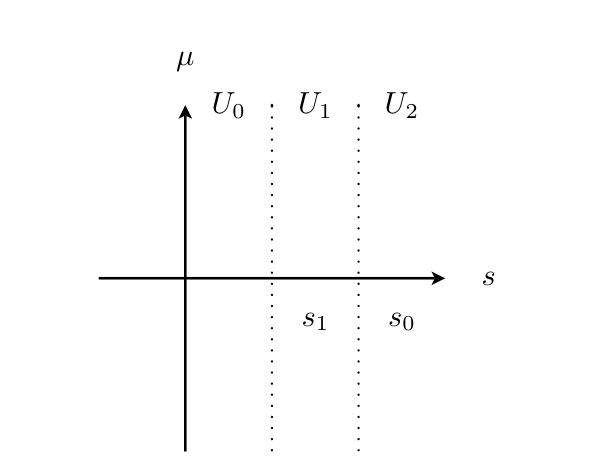
\includegraphics[width=0.5\textwidth]{figures/fig31.1.png}
  \figtitle{31.1}{底空间上的判别式与墙}
\end{figure}

\begin{figure}[htbp]
  \centering
  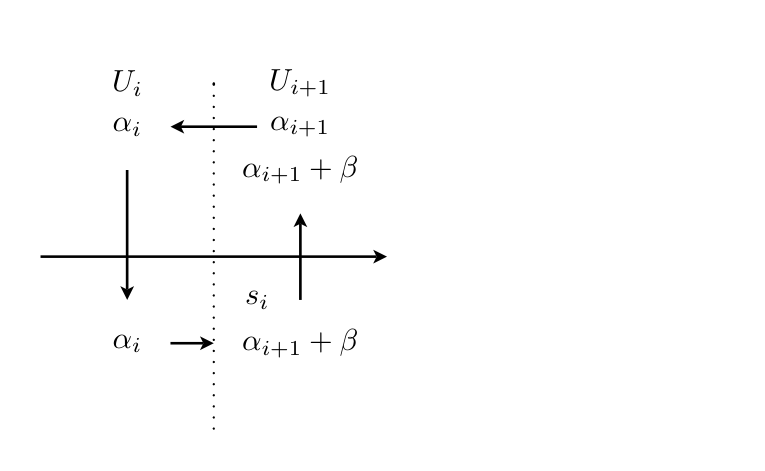
\includegraphics[width=0.55\textwidth]{figures/fig31.2.png}
  \figtitle{31.2}{单值}
\end{figure}

\begin{figure}[htbp]
  \centering
  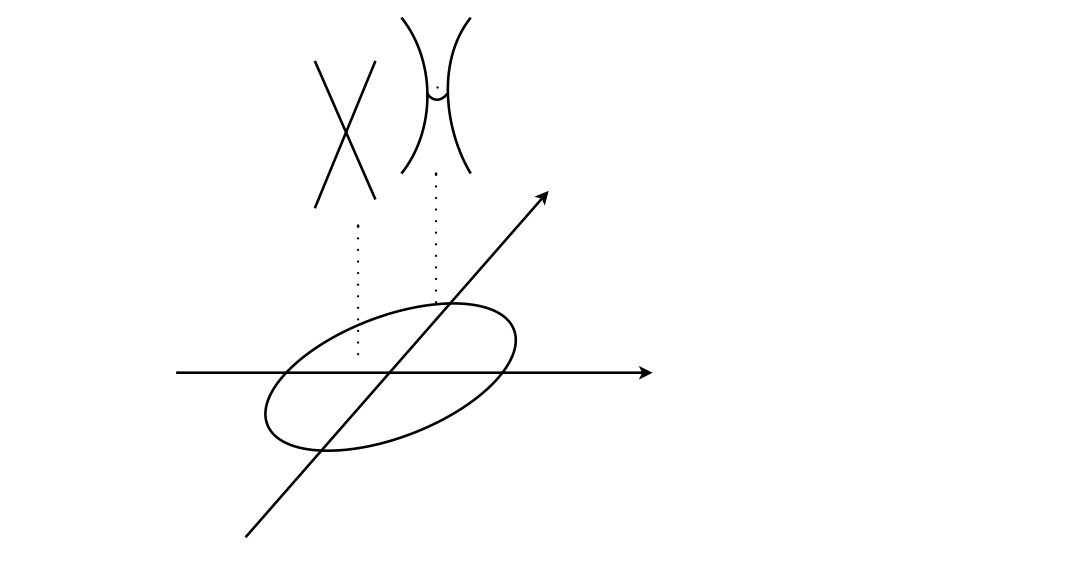
\includegraphics[width=0.6\textwidth]{figures/fig31.3.png}
  \figtitle{31.3}{拉格朗日环面}
\end{figure}

在 $b \in U_i$ 处 $H_1(L_b;\Z)$ 的基由
\begin{equation}
\alpha_i := \left\{(z,u,v) \in L_b \;\middle|\; z = r\ee^{2\pi\sqrt{-1}\theta}\text{，且 } u \text{ 与 } v \text{ 绕原点的卷绕数分别为 } 0 \text{ 与 } i\right\}, \tag{31.14}
\end{equation}
\begin{equation}
\beta := \left\{(z,u,v) \in L_b \;\middle|\; z = r,\ u = |u|\cdot\ee^{2\pi\sqrt{-1}\theta},\ v = |v|\cdot\ee^{-2\pi\sqrt{-1}\theta}\right\} \tag{31.15}
\end{equation}
给出。注意在 $\beta$ 的定义中，固定 $z$ 时 $|u|$ 与 $|v|$ 是被固定的。$\alpha_i$ 依赖于 $i$，而 $\beta$ 不依赖于 $i$。

同调类 $\alpha \in H_1(L_b;\Z)$ 对一切 $b \in \R^2 \setminus \Gamma$ 都有定义，而 $\beta_i$ 在 $\Gamma$ 的周围具有单值。若把 $\beta_i$ 从 $U_i$ 通过 $\mu > 0$ 的区域移动到 $U_{i+1}$，则这里恒有 $u > 0$，同时 $z = a_i$ 处 $v = 0$。因此可知，在此操作下 $\varphi_u$ 不变，而 $\varphi_v$ 只增加 $1$。同样地，若把 $\beta_i$ 从 $U_i$ 通过 $\mu < 0$ 的区域移动到 $U_{i+1}$，则 $\varphi_u$ 只增加 $1$，而 $\varphi_v$ 保持不变。

$\alpha_i$ 与 $\beta$ 对应的卷绕数 $(\varphi_z, \varphi_u, \varphi_v)$ 分别为 $(1,0,i)$ 及 $(0,1,-1)$，而在 $s_i \in \Gamma$ 的周围圈的单值，可由图 31.2 读出为
\begin{align}
\alpha_{i+1} &\mapsto \alpha_{i+1} + \beta \tag{31.16}\\
\beta &\mapsto \beta \tag{31.17}
\end{align}

\begin{figure}[htbp]
  \centering
  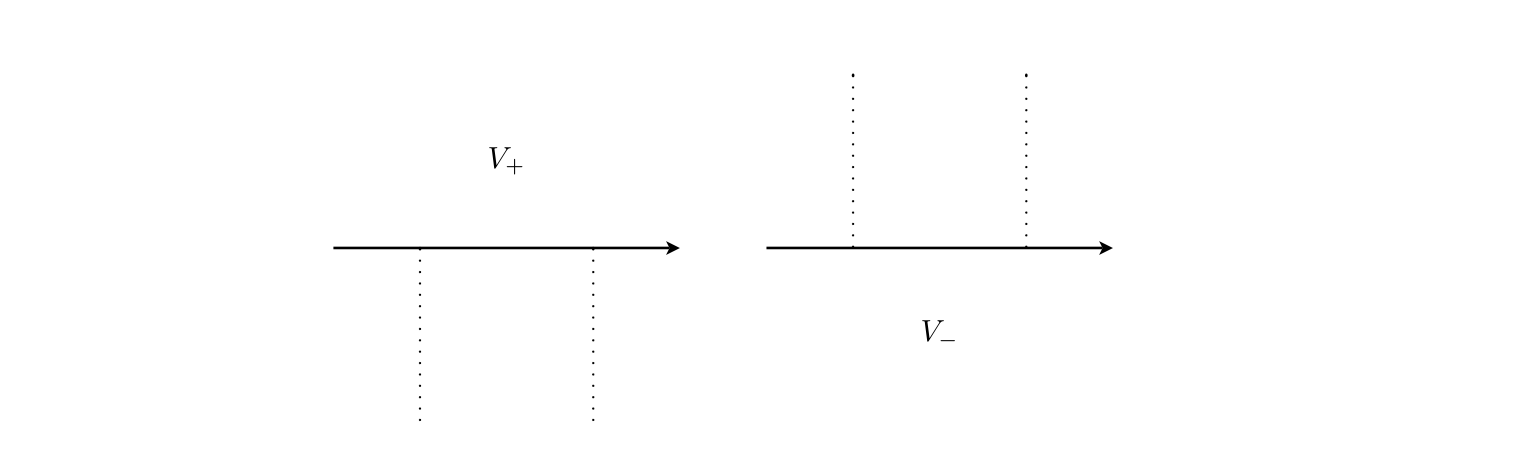
\includegraphics[width=0.6\textwidth]{figures/fig31.4.png}
  \figtitle{31.4}{两个开集}
\end{figure}

从判别式集合 $\Gamma$ 沿单值不变的方向延伸所得的直线 $\{s = s_i\}$ 称为墙（wall）。$\R^2 \setminus \Gamma$ 可用除去墙的下半与上半所得的集合
\begin{align}
V_+ &= \R^2 \setminus \left\{(s_i,\mu) \in \R^2 \mid i = 0,1,\ \mu \le 0\right\}, \tag{31.18}\\
V_- &= \R^2 \setminus \left\{(s_i,\mu) \in \R^2 \mid i = 0,1,\ \mu \ge 0\right\} \tag{31.19}
\end{align}
写成 $V_+ \cup V_-$。$V_+ \cap V_- = U_0 \sqcup U_1 \sqcup U_2$，而 $B_0$ 的仿射结构由把 $V_+$ 与 $V_-$ 的标准仿射结构按转换函数
\begin{equation}
\phi_{V_-,V_+}(s,\mu) = \begin{cases}
(s,\mu) & (s,\mu) \in U_0\\
(s,s+\mu) & (s,\mu) \in U_1\\
(s,2s+\mu) & (s,\mu) \in U_2
\end{cases} \tag{31.20}
\end{equation}
黏合而得。

在 $(s_0,0)$ 与 $(s_1,0)$ 处 $B$ 的奇点称为焦点-焦点奇点（focus-focus singularity）。由 Gauss--Bonnet 型定理可知：容许至多带焦点-焦点奇点的热带仿射结构的紧 $2$ 维流形只有球面、实射影平面、环面及 Klein 瓶这 $4$ 种；且各情形下焦点-焦点奇点的个数必须分别为 $24$ 个、$12$ 个、$0$ 个、$0$ 个 [LS10]。对应的辛流形分别是 K3 曲面、Enriques 曲面、环面上的环面丛、Klein 瓶上的环面丛。

\section{热带几何}

无奇点的紧热带仿射流形只限于仿射空间对离散群的商空间，因此要构造其他例子就无法回避奇点。置判别式集合的补集为 $B^{\mathrm{sm}} := B \setminus \Gamma$，则 $TB^{\mathrm{sm}}/T_{\Z}B^{\mathrm{sm}}$ 具有半平坦复结构；但为把它延拓到判别式集合，据信需要由全纯圆盘计数给出的瞬子修正 [Fuk05]。这种瞬子修正是非局部的，具体计算一般极为困难。

另一方面，对给定的热带仿射流形，可以考察半平坦复结构的自然单参数族
\begin{equation}
X_\epsilon(B_0) := TB_0/tT_{\Z}B_0 \tag{32.1}
\end{equation}
例如当 $B = B^{\mathrm{sm}} := \R/r\Z$ 是半径为 $r$ 的圆周时，对应的单参数族为
\begin{align}
X_\epsilon(B) &:= TS^1/tT_{\Z}S^1 \tag{32.2}\\
&= \C/\left(t\Z + \sqrt{-1}r\Z\right) \tag{32.3}\\
&\cong \C/\left(\Z + t^{-1}r\sqrt{-1}\Z\right) \tag{32.4}
\end{align}
可见在令 $\epsilon$ 趋于 $0$ 的极限下周期趋于无穷大。

\begin{figure}[htbp]
  \centering
  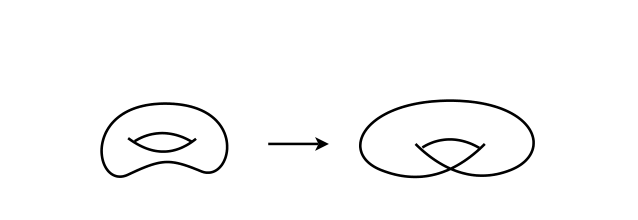
\includegraphics[width=0.4\textwidth]{figures/fig32.1.png}
  \figtitle{32.1}{代数几何意义下的退化}
\end{figure}

\begin{figure}[htbp]
  \centering
  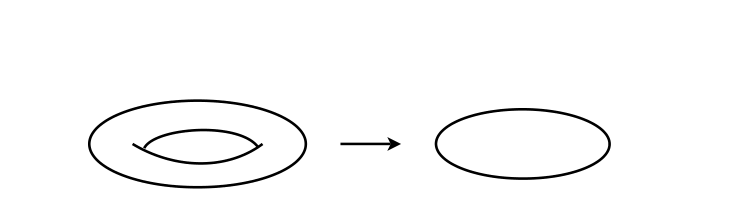
\includegraphics[width=0.4\textwidth]{figures/fig32.2.png}
  \figtitle{32.2}{Gromov--Hausdorff 收敛}
\end{figure}

在这个退化的代数几何模型中，如图 32.1 所示，曲线逐渐被掐细，极限是带结点的有理曲线。另一方面，在 Ricci 平坦的模型中保持直径不变地变形复结构时，则如图 32.2 所示曲线变细，极限是圆周。在代数几何的退化模型中曲率集中的地方，在 Ricci 平坦的模型中几乎是整体。一般地，热带仿射流形对应的不是单个复流形，而是复流形的退化族。

定义依赖于正参数 $t$ 的加法与乘法的变形为
\begin{equation}
x \oplus_t y := -\log_t\left(t^{-x} + t^{-y}\right),\quad x \odot_t y := x + y \tag{32.5}
\end{equation}
则其在 $t \to 0$ 时的极限为
\begin{equation}
x \oplus y := \max\{x,y\},\quad x \odot y := x + y \tag{32.6}
\end{equation}

对收敛 Puiseux 级数环 $\mathbb{K} := \bigcup_{n=1}^{\infty}\C((T^{1/n}))$ 的赋值 $v: \mathbb{K} \to \Q \cup \{\infty\}$ 与绝对值 $|\cdot|: \mathbb{K} \to \R$，对 $x = a_pT^p + a_{p+1/n}T^{p+1/n} + \cdots$（$a_p \ne 0$）定义为 $v(x) = p$ 与 $|x| = \ee^{-p}$。另外，$0$ 的赋值与绝对值分别定义为 $\infty$ 及 $0$。

设 $\boldsymbol{M}$ 为秩 $n$ 的自由 Abel 群，$\boldsymbol{N} := \Hom(\boldsymbol{M}, \Z)$ 为其对偶 Abel 群。对 Laurent 多项式
\begin{equation}
f = \sum_{m \in \boldsymbol{M}} a_m x^{n} \in \mathbb{K}[\boldsymbol{M}] \tag{32.7}
\end{equation}
定义其热带化为
\begin{equation}
f_{\mathrm{trop}}(x) := \max_{m \in \boldsymbol{M}}\left\{v(a_m) + \langle m,x\rangle\right\} \tag{32.8}
\end{equation}
则它确定 $\boldsymbol{N}_{\R} := \boldsymbol{N} \otimes \R$ 上的分片仿射函数，称之为伴随 $f$ 的热带多项式。定义热带多项式 $f_{\mathrm{trop}}$ 所定热带超曲面为
\begin{equation}
V(f_{\mathrm{trop}}) := \left\{x \in \boldsymbol{N}_{\R} \mid f_{\mathrm{trop}} \text{ 在 } x \text{ 处不可微}\right\} \tag{32.9}
\end{equation}
又，置
\begin{equation}
\operatorname{Log} : \boldsymbol{N}_{\mathbb{K}} \to \boldsymbol{N}_{\R},\quad (x_i)_{i=1}^{n} \mapsto (\log|x_i|)_{i=1}^{n} \tag{32.10}
\end{equation}

\begin{theorem}[{[EKL06, Theorem 2.1.1]}]
热带超曲面 $V(f_{\mathrm{trop}})$ 与 $\operatorname{Log}\left(f^{-1}(0)\right)$ 的闭包一致。
\end{theorem}

对正数 $t$，把 Laurent 多项式 $f$ 的系数中出现的 Puiseux 级数的不定元 $T$ 代入 $t$ 所得的 Laurent 多项式记作 $f_t \in \C[\boldsymbol{M}]$。又，置
\begin{equation}
\operatorname{Log}_t : \boldsymbol{N}_{\C}^{\times} \to \boldsymbol{N}_{\R},\quad (z_i)_{i=1}^{n} \mapsto (\log_t|z_i|)_{i=1}^{n} \tag{32.11}
\end{equation}

\begin{theorem}[{[Mik04, Corollary 6.4]}]
关于 $\boldsymbol{N}_{\R}$ 的 Hausdorff 拓扑，
\begin{equation}
\lim_{t \to 0}\operatorname{Log}_t\left(f_t^{-1}(0)\right) = V(f_{\mathrm{trop}}) \tag{32.12}
\end{equation}
成立。
\end{theorem}

\section{Berkovich 空间}

% [Tutor Note: 本节原文以粗体 k 记基域，故此处统一写 \mathbf{k}（preamble 的 \kk 为普通 k，未采用）。]

设 $\mathbf{k}$ 为域。若映射 $v_{\mathbf{k}} : \mathbf{k} \to \R \cup \{\infty\}$ 对任意 $x, y \in \mathbf{k}$ 满足
\begin{enumerate}[label=\arabic*.]
\item $v_{\mathbf{k}}(x) = \infty \Leftrightarrow x = 0$
\item $v_{\mathbf{k}}(xy) = v_{\mathbf{k}}(x) + v_{\mathbf{k}}(y)$
\item $v_{\mathbf{k}}(x+y) \ge \min\{v_{\mathbf{k}}(x), v_{\mathbf{k}}(y)\}$
\end{enumerate}
则称 $v_{\mathbf{k}}$ 为非阿基米德赋值（non-Archimedean valuation）。由非阿基米德赋值，非阿基米德绝对值（non-Archimedean absolute value）$|\cdot|_{\mathbf{k}} : \mathbf{k} \to \R^{\ge 0}$ 由
\begin{equation}
|\cdot|_{\mathbf{k}} = \ee^{-v_{\mathbf{k}}(\cdot)} \tag{33.1}
\end{equation}
确定，而条件 3 被翻译为非阿基米德三角不等式
\begin{itemize}
\item $|x+y|_{\mathbf{k}} \le \max\left\{|x|_{\mathbf{k}}, |y|_{\mathbf{k}}\right\}$
\end{itemize}
域 $\mathbf{k}$ 与其上的非阿基米德绝对值 $|\cdot|_{\mathbf{k}}$ 的组 $(\mathbf{k}, |\cdot|_{\mathbf{k}})$，若非阿基米德绝对值所定的距离 $d(x,y) := |x-y|_{\mathbf{k}}$ 使其完备，则称为非阿基米德域（non-Archimedean field）。

作为复解析几何对非阿基米德域的类似物，有 Tate 的刚性解析空间（Tate's rigid analytic space）[Tat71]、Raynaud 一般纤维（Raynaud generic fiber）[Ray74]、Berkovich 解析空间（Berkovich's analytic space）[Ber90]、Huber 的 adic 空间（Huber's adic space）[Hub93]、藤原--加藤的 Zariski--Riemann 空间 [FK] 等；综述文章可举 [Kat98, Kat03, Con08, Bak08, Tem15, Pay15] 等。以下沿 [KS06]，使用 Berkovich 解析空间。

$\mathbf{k}$ 上的线性空间 $V$ 与映射 $\|\cdot\| : V \to \R^{\ge 0}$ 的组 $(V, \|\cdot\|)$，若对任意 $v, v' \in V$ 与任意 $c \in \mathbf{k}$ 满足
\begin{enumerate}[label=\arabic*.]
\item $\|v + v'\| \le \max\left(\|v\|, \|v'\|\right)$
\item $\|cv\| = |c|_{\mathbf{k}}\|v\|$
\item $\|v\| = 0 \Leftrightarrow v = 0$
\end{enumerate}
则称为 $\mathbf{k}$ 上的 Banach 空间（$\mathbf{k}$-Banach space）。若 $\mathbf{k}$ 上的 Banach 空间 $A$ 具有 $\mathbf{k}$-代数结构，且任意 $a, b \in A$ 满足
\begin{equation}
\|ab\| \le \|a\| \cdot \|b\| \tag{33.2}
\end{equation}
则称 $A$ 为 $\mathbf{k}$ 上的 Banach 代数（$\mathbf{k}$-Banach algebra）。$\mathbf{k}$ 上 Banach 代数 $A$ 的半范数（seminorm）是指满足
\begin{enumerate}[label=\arabic*.]
\item $|0| = 0$
\item $|1| = 1$
\item $|f+g| \le |f| + |g|$
\item $|fg| \le |f|\,|g|$
\end{enumerate}
的映射 $|\cdot| : A \to \R^{\ge 0}$。满足「若 $|f| = 0$ 则 $f = 0$」的半范数 $|\cdot|$ 称为范数。半范数满足 $|fg| = |f|\,|g|$ 时称为乘性的（multiplicative）；半范数满足 $|f| \le \|f\|$ 时称为有界的（bounded）。对 Banach 代数 $A$，在 $A$ 的有界乘性半范数之集合上赋以使映射
\begin{equation}
\mathcal{M}(A) \to \R^{\ge 0},\quad |\cdot| \mapsto |f| \tag{33.3}
\end{equation}
对任意 $f \in A$ 都连续的最弱拓扑，所得空间称为 $A$ 的 Berkovich 谱（Berkovich spectrum），记作 $\mathcal{M}(A)$。

对 $r_1, \dots, r_n > 0$，在
\begin{equation}
\mathbf{k}\left\langle r_1^{-1}X_1, \dots, r_n^{-1}X_n\right\rangle := \left\{\sum_{J} a_J T^J \in K[[X_1, \dots, X_n]] \;\middle|\; |a_J|_{\mathbf{k}}\, r^J \to 0\right\} \tag{33.4}
\end{equation}
上赋以 Gauss 范数
\begin{equation}
\left\|\sum_{J} a_J X^J\right\| := \sup_{J} |a_J|_K\, r^J \tag{33.5}
\end{equation}
所得的 Banach 代数称为变形 Tate 代数（modified Tate algebra）。若 $\mathbf{k}$ 上的 Banach 代数 $A$ 具有从某个变形 Tate 代数出发的满射，且其范数由该变形 Tate 代数的 Gauss 范数诱导，则称 $A$ 为 $\mathbf{k}$-affinoid 代数（$\mathbf{k}$-affinoid algebra）。$\mathbf{k}$-affinoid 代数的 Berkovich 谱称为 affinoid 区域（affinoid domain）。把 affinoid 区域沿适当的 Grothendieck 拓扑黏合所得的空间，称为 Berkovich 解析空间（Berkovich's analytic space）或简称为 Berkovich 空间。存在从 $\mathbf{k}$ 上代数簇的范畴到 Berkovich 空间的范畴、称为解析化（analytification）的函子 $(\cdot)^{\mathrm{an}}$。

定义代数环面 $\mathbb{G}_m^n := \Spec \mathbf{k}[z_1^{\pm 1}, \dots, z_n^{\pm n}]$ 的解析化 $(\mathbb{G}_m^n)^{\mathrm{an}}$ 到 $\R^n$ 的映射为
\begin{equation}
\pi_{\mathrm{can}} : (\mathbb{G}_m^n)^{\mathrm{an}} \to \R^n,\quad x \mapsto (\log|z_1(x)|, \dots, \log|z_n(x)|) \tag{33.6}
\end{equation}
$\mathbf{k}$-代数的层 $\cO^{\mathrm{can}}_{\R^n}$ 由
\begin{equation}
\cO^{\mathrm{can}}_{\R^n}(U) = \left\{f \in \sum_{\omega \in \Z^n} a_\omega z^\omega \;\middle|\; \forall x \in U,\ \lim_{|\omega| \to \infty} \log|a_\omega| + \langle x,\omega\rangle \to \infty = \infty\right\} \tag{33.7}
\end{equation}
定义。

若从 Berkovich 空间到 Hausdorff 空间的映射 $\pi : X \to B^{\mathrm{sm}}$ 满足：对任意 $b \in B^{\mathrm{sm}}$，存在 $b$ 的邻域 $U$ 与 $\R^n$ 的开集 $V$，使图表
\begin{equation}
\begin{array}{ccc}
\pi^{-1}(U) & \xrightarrow{\ \sim\ } & \pi_{\mathrm{can}}^{-1}(V)\\[4pt]
\downarrow & & \downarrow\\[4pt]
U & \xrightarrow{\ \sim\ } & V
\end{array} \tag{33.8}
\end{equation}
交换，则称 $\pi$ 为解析环面纤维化（analytic torus fibration）。其中上行为 Berkovich 空间的同构，下行为同胚。解析环面纤维化的底空间具有这样的热带仿射结构：由
\begin{equation}
\operatorname{Aff}_{\Z,B^{\mathrm{sm}}}(U) := \left\{v(f) + c \mid f \in \cO(\pi^{-1}(U))^{\times},\ c \in \R\right\} \tag{33.9}
\end{equation}
定义的层 $\operatorname{Aff}_{\Z,B^{\mathrm{sm}}}$ 是热带仿射函数构成的层。反之，给定热带仿射流形 $B^{\mathrm{sm}}$ 时，通过黏合 affinoid 区域，可以构造 Berkovich 空间 $X$ 与解析环面纤维化 $\pi : X \to B^{\mathrm{sm}}$。

\begin{question}
$B$ 取 $\R^2$ 的具有热带仿射结构、且在原点有焦点-焦点奇点者。此时，试构造 Berkovich 曲面 $X$ 与连续映射 $\pi : X \to B$，使其在原点之外是解析环面纤维化，并在该处具有给定的热带仿射结构。
\end{question}

此问题由 Kontsevich--Soibelmann 如下解决：首先，把 $(\mathbb{G}_m^{\mathrm{an}})^2$ 的两个副本沿公共部分按
\begin{equation}
\left\{
\begin{array}{rcl}
z'_1 & = & (1+z_2)z_1\\
z'_2 & = & z_2
\end{array}
\right. \tag{33.10}
\end{equation}
黏合，再取部分紧致化，便得到
\begin{equation}
X = \Spec \mathbf{k}[\alpha,\beta,\gamma]/((\alpha\beta-1)\gamma-1) \tag{33.11}
\end{equation}
的解析化 $X^{\mathrm{an}}$。这里 $(\alpha,\beta,\gamma)$ 与 $(z_1,z_2)$、$(z'_1,z'_2)$ 由
\begin{equation}
\alpha = \frac{1}{z_1},\quad \beta = z'_1,\quad \gamma = \frac{1}{z_2} = \frac{1}{z'_2} \tag{33.12}
\end{equation}
相联系。注意由 (33.10) 可得
\begin{align}
v(z'_1) &= v(1+z_2) + v(z_1) \tag{33.13}\\
&= \min\{0, v(z_2)\} + v(z_1) \tag{33.14}\\
&= \begin{cases}
v(z_1) & v(z_2) \ge 0,\\
v(z_1) + v(z_2) & v(z_2) \le 0
\end{cases} \tag{33.15}
\end{align}

\section{$A_1$ 奇点}

镜像由把
\begin{equation}
X = \Spec \mathbf{k}[\alpha,\beta,\gamma]/((\alpha\beta-1)\gamma-1) \tag{34.1}
\end{equation}
与
\begin{equation}
X' = \Spec \mathbf{k}[\alpha',\beta',\gamma']/((\alpha'\beta'-1)\gamma'-1) \tag{34.2}
\end{equation}
按
\begin{equation}
\alpha = \frac{1}{\alpha'},\quad \beta = (\alpha')^2\beta',\quad \gamma = \gamma' \tag{34.3}
\end{equation}
黏合而得。所得空间与把 $\mathbb{A}^2 \setminus \{0\}$ 对 $\mathbb{G}_m$ 的作用 $(z,w,\zeta) \mapsto (\delta z, \delta w, \delta^{-2}\zeta)$ 取商所得的空间
\begin{equation}
K_{\PP^1} \cong \left((\mathbb{A}^2 \setminus \{0\})/\mathbb{G}_m,\right. \tag{34.4}
\end{equation}
的开集通过
\begin{equation}
X \to K_{\PP^1},\quad (\alpha,\beta,\gamma) \mapsto [1,\alpha,\beta], \tag{34.5}
\end{equation}
\begin{equation}
X' \to K_{\PP^1},\quad (\alpha',\beta',\gamma') \mapsto [\alpha',1,\beta'] \tag{34.6}
\end{equation}
同构。

% [Tutor Note: 原文的若干疑似排印问题，均照录图像、未作改动：
%  (a) (32.7) 中 $a_m x^{n}$ 的上标原文印作 $n$（按上下文疑为 $m$）；
%  (b) p046 的 Puiseux 级数环印作黑板的 $\mathbb{K}$，而 p048 的 (33.4)(33.5) 中同一对象
%      印作斜体 $K$；
%  (c) (33.6) 上方 $\Spec \mathbf{k}[z_1^{\pm 1},\dots,z_n^{\pm n}]$ 的末个指数原文印作 $\pm n$
%      （按惯例疑为 $\pm 1$）；
%  (d) (33.7) 中条件原文印作「$\lim_{|\omega|\to\infty}\log|a_\omega| + \langle x,\omega\rangle
%      \to \infty = \infty$」，末尾「$= \infty$」语义重复，照录；
%  (e) (34.4) 的括号在原文中于「$K_{\PP^1} \cong ((\mathbb{A}^2\setminus\{0\})/\mathbb{G}_m,$」
%      处未闭合（下接「の開集合と」），照录；
%  (f) 人名原文作「Kontsevich--Soibelmann」，通行拼写为「Kontsevich--Soibelman」，照录原文。]

% （p049 末尾的「参考文献」标题与首 3 条已由 Lead 并入 c12.tex，此处不再重复。）


% CHUNK c11 DONE pages p043–p049

% c12 —— 参考文献（Lead 整理；条目保留原文，仅做连字与重音清理）
\clearpage
\section*{参考文献}
\addcontentsline{toc}{section}{参考文献}
{\small
\setlength{\parindent}{0pt}
\begin{list}{}{%
  \setlength{\leftmargin}{3.4em}%
  \setlength{\itemindent}{-3.4em}%
  \setlength{\itemsep}{1.5pt}%
  \setlength{\parsep}{0pt}%
  \setlength{\listparindent}{0pt}%
}
\item[{[AAE+13]}] Mohammed Abouzaid, Denis Auroux, Alexander I. Efimov, Ludmil Katzarkov, and Dmitri Orlov, \textit{Homological mirror symmetry for punctured spheres}, J. Amer. Math. Soc. \textbf{26} (2013), no. 4, 1051--1083. MR 3073884
\item[{[ABC+09]}] Paul S. Aspinwall, Tom Bridgeland, Alastair Craw, Michael R. Douglas, Mark Gross, Anton Kapustin, Gregory W. Moore, Graeme Segal, Balázs Szendrői, and P. M. H. Wilson, \textit{Dirichlet branes and mirror symmetry}, Clay Mathematics Monographs, vol. 4, American Mathematical Society, Providence, RI; Clay Mathematics Institute, Cambridge, MA, 2009. MR 2567952 (2011e:53148)
\item[{[Aboa]}] Mohammed Abouzaid, \textit{Family Floer cohomology and mirror symmetry}, arXiv:1404.2659.
\item[{[Abob]}] , The family Floer functor is faithful, arXiv:1408.6794.
\item[{[Abo06]}] , Homogeneous coordinate rings and mirror symmetry for toric varieties, Geom. Topol. 10 (2006), 1097--1157 (electronic). MR MR2240909 (2007h:14052)
\item[{[Abo09]}] , Morse homology, tropical geometry, and homological mirror symmetry for toric varieties, Selecta Math. (N.S.) 15 (2009), no. 2, 189--270. MR MR2529936
\item[{[Abo11]}] , A topological model for the Fukaya categories of plumbings, J. Differential Geom. 87 (2011), no. 1, 1--80. MR 2786590 (2012h:53193)
\item[{[AGV08]}] Dan Abramovich, Tom Graber, and Angelo Vistoli, Gromov-Witten theory of Deligne-Mumford stacks, Amer. J. Math. 130 (2008), no. 5, 1337--1398. MR 2450211 (2009k:14108)
\item[{[AGZV85]}] V. I. Arnol′d, S. M. Guseĭn-Zade, and A. N. Varchenko, Singularities of differentiable maps. Vol. I, Monographs in Mathematics, vol. 82, Birkhäuser Boston Inc., Boston, MA, 1985, The classification of critical points, caustics and wave fronts, Translated from the Russian by Ian Porteous and Mark Reynolds. MR 777682 (86f:58018)
\item[{[AKO06]}] Denis Auroux, Ludmil Katzarkov, and Dmitri Orlov, Mirror symmetry for del Pezzo surfaces: van- ishing cycles and coherent sheaves, Invent. Math. 166 (2006), no. 3, 537--582. MR MR2257391 (2007g:14045)
\item[{[AKO08]}] , Mirror symmetry for weighted projective planes and their noncommutative deformations, Ann. of Math. (2) 167 (2008), no. 3, 867--943. MR MR2415388 (2009f:53142)
\item[{[AMRT10]}] Avner Ash, David Mumford, Michael Rapoport, and Yung-Sheng Tai, Smooth compactifications of locally symmetric varieties, second ed., Cambridge Mathematical Library, Cambridge University Press, Cambridge, 2010, With the collaboration of Peter Scholze. MR 2590897 (2010m:14067)
\item[{[AS10a]}] Mohammed Abouzaid and Paul Seidel, An open string analogue of Viterbo functoriality, Geom. Topol. 14 (2010), no. 2, 627--718. MR 2602848 (2011g:53190)
\item[{[AS10b]}] Mohammed Abouzaid and Ivan Smith, Homological mirror symmetry for the 4-torus, Duke Math. J. 152 (2010), no. 3, 373--440. MR 2654219 (2011d:53218)
\item[{[Aur07]}] Denis Auroux, Mirror symmetry and T -duality in the complement of an anticanonical divisor, J. Gökova Geom. Topol. GGT 1 (2007), 51--91. MR 2386535 (2009f:53141)
\item[{[Aur09]}] , Special Lagrangian fibrations, wall-crossing, and mirror symmetry, Surveys in differential geometry. Vol. XIII. Geometry, analysis, and algebraic geometry: forty years of the Journal of Differential Geometry, Surv. Differ. Geom., vol. 13, Int. Press, Somerville, MA, 2009, pp. 1--47. MR MR2537081
\item[{[Bak08]}] Matthew Baker, An introduction to Berkovich analytic spaces and non-Archimedean potential theory on curves, p-adic geometry, Univ. Lecture Ser., vol. 45, Amer. Math. Soc., Providence, RI, 2008, pp. 123--174. MR 2482347 (2010g:14029)
\item[{[Bal]}] Matthew Robert Ballard, Sheaves on local Calabi-Yau varieties, arXiv:0801.3499.
\item[{[Bal08]}] , Meet homological mirror symmetry, Modular forms and string duality, Fields Inst. Com- mun., vol. 54, Amer. Math. Soc., Providence, RI, 2008, pp. 191--224. MR 2454326 (2009m:53225)
\item[{[Bat94]}] Victor V. Batyrev, Dual polyhedra and mirror symmetry for Calabi-Yau hypersurfaces in toric va- rieties, J. Algebraic Geom. 3 (1994), no. 3, 493--535. MR MR1269718 (95c:14046)
\item[{[Bat98]}] , Stringy Hodge numbers of varieties with Gorenstein canonical singularities, Integrable sys- tems and algebraic geometry (Kobe/Kyoto, 1997), World Sci. Publ., River Edge, NJ, 1998, pp. 1--32. MR 1672108 (2001a:14039)
\item[{[BB96]}] Victor V. Batyrev and Lev A. Borisov, Mirror duality and string-theoretic Hodge numbers, Invent. Math. 126 (1996), no. 1, 183--203. MR 1408560 (97k:14039)
\item[{[BBD82]}] A. A. Beĭlinson, J. Bernstein, and P. Deligne, Faisceaux pervers, Analysis and topology on singular spaces, I (Luminy, 1981), Astérisque, vol. 100, Soc. Math. France, Paris, 1982, pp. 5--171. MR MR751966 (86g:32015)
\item[{[BD96]}] Victor V. Batyrev and Dimitrios I. Dais, Strong McKay correspondence, string-theoretic Hodge numbers and mirror symmetry, Topology 35 (1996), no. 4, 901--929. MR 1404917 (97e:14023)
\item[{[Ber90]}] Vladimir G. Berkovich, Spectral theory and analytic geometry over non-Archimedean fields, Math- ematical Surveys and Monographs, vol. 33, American Mathematical Society, Providence, RI, 1990. MR 1070709 (91k:32038)
\item[{[BFK]}] Matthew Ballard, David Favero, and Ludmil Katzarkov, Variation of geometric invariant theory quotients and derived categories, arXiv:1203.6643.
\item[{[BH93]}] Per Berglund and Tristan Hübsch, A generalized construction of mirror manifolds, Nuclear Phys. B 393 (1993), no. 1-2, 377--391. MR MR1214325 (94k:14031)
\item[{[BK90]}] A. I. Bondal and M. M. Kapranov, Enhanced triangulated categories, Mat. Sb. 181 (1990), no. 5, 669--683. MR MR1055981 (91g:18010)
\item[{[BLM08]}] Yu. Bespalov, V. Lyubashenko, and O. Manzyuk, Pretriangulated A∞-categories, Proceedings of Institute of Mathematics of NAS of Ukraine. Mathematics and its Applications, vol. 76, Nats¯ional′na Akadem¯iya Nauk Ukra¨ini, ¯Institut Matematiki, Kiev, 2008. MR 2513383 (2010j:18019)
\item[{[BO]}] Alexei Bondal and Dmitri Orlov, Semiorthogonal decomposition for algebraic varieties, arXiv:alg- geom/9506012.
\item[{[BO02]}] A. Bondal and D. Orlov, Derived categories of coherent sheaves, Proceedings of the International Congress of Mathematicians, Vol. II (Beijing, 2002), Higher Ed. Press, Beijing, 2002, pp. 47--56. MR 1957019 (2003m:18015)
\item[{[Boc16]}] Raf Bocklandt, Noncommutative mirror symmetry for punctured surfaces, Trans. Amer. Math. Soc. 368 (2016), no. 1, 429--469. MR 3413869
\item[{[Bor13]}] Lev A. Borisov, Berglund-Hübsch mirror symmetry via vertex algebras, Comm. Math. Phys. 320 (2013), no. 1, 73--99. MR 3046990
\item[{[Bri02]}] Tom Bridgeland, Flops and derived categories, Invent. Math. 147 (2002), no. 3, 613--632. MR MR1893007 (2003h:14027)
\item[{[Buc87]}] Ragnar-Olaf Buchweitz, Maximal Cohen-Macaulay modules and Tate-cohomology over Gorenstein rings, Available from https://tspace.library.utoronto.ca/handle/1807/16682, 1987.
\item[{[BZN12]}] David Ben-Zvi and David Nadler, Loop spaces and connections, J. Topol. 5 (2012), no. 2, 377--430. MR 2928082
\item[{[BZN13]}] , Loop spaces and representations, Duke Math. J. 162 (2013), no. 9, 1587--1619. MR 3079256
\item[{[CdlOGP91]}] Philip Candelas, Xenia C. de la Ossa, Paul S. Green, and Linda Parkes, A pair of Calabi-Yau manifolds as an exactly soluble superconformal theory, Nuclear Phys. B 359 (1991), no. 1, 21--74. MR MR1115626 (93b:32029)
\item[{[CdlOGP92]}] , A pair of Calabi-Yau manifolds as an exactly soluble superconformal theory, Essays on mirror manifolds, Internat. Press, Hong Kong, 1992, pp. 31--95. MR MR1191420
\item[{[CHL]}] Cheol-Hyun Cho, Hansol Hong, and Siu-Cheong Lau, Localized mirror functor for Lagrangian im- mersions, and homological mirror symmetry for P1 a,b,c, arXiv:1308.4651.
\item[{[Cib00]}] Claude Cibils, Tensor Hochschild homology and cohomology, Interactions between ring theory and representations of algebras (Murcia), Lecture Notes in Pure and Appl. Math., vol. 210, Dekker, New York, 2000, pp. 35--51. MR 1758400 (2001i:16016)
\item[{[CIR14]}] Alessandro Chiodo, Hiroshi Iritani, and Yongbin Ruan, Landau-Ginzburg/Calabi-Yau correspon- dence, global mirror symmetry and Orlov equivalence, Publ. Math. Inst. Hautes ´Etudes Sci. 119 (2014), 127--216. MR 3210178
\item[{[CK99]}] David A. Cox and Sheldon Katz, Mirror symmetry and algebraic geometry, Mathematical Surveys and Monographs, vol. 68, American Mathematical Society, Providence, RI, 1999. MR MR1677117 (2000d:14048)
\item[{[Cla]}] Patrick Clarke, Duality for toric Landau-Ginzburg models, arXiv:0803.0447.
\item[{[Cle87]}] Herbert Clemens, Curves on higher-dimensional complex projective manifolds, Proceedings of the International Congress of Mathematicians, Vol. 1, 2 (Berkeley, Calif., 1986), Amer. Math. Soc., Providence, RI, 1987, pp. 634--640. MR 934266 (89e:14007)
\item[{[CLS90]}] P. Candelas, M. Lynker, and R. Schimmrigk, Calabi-Yau manifolds in weighted P4, Nuclear Phys. B 341 (1990), no. 2, 383--402. MR 1067295 (91m:14062)
\item[{[Coh]}] Lee Cohn, Differential graded categories are k-linear stable infinity categories, arXiv:1308.2587.
\item[{[Con08]}] Brian Conrad, Several approaches to non-Archimedean geometry, p-adic geometry, Univ. Lecture Ser., vol. 45, Amer. Math. Soc., Providence, RI, 2008, pp. 9--63. MR 2482345 (2011a:14047)
\item[{[Cos07]}] Kevin Costello, Topological conformal field theories and Calabi-Yau categories, Adv. Math. 210 (2007), no. 1, 165--214. MR 2298823 (2008f:14071)
\item[{[CPU]}] Kwokwai Chan, Daniel Pomerleano, and Kazushi Ueda, Lagrangian torus fibrations and homological mirror symmetry for the conifold, accepted for publication in Comm. Math. Phys., arXiv:1305.0968.
\item[{[CR02]}] Weimin Chen and Yongbin Ruan, Orbifold Gromov-Witten theory, Orbifolds in mathematics and physics (Madison, WI, 2001), Contemp. Math., vol. 310, Amer. Math. Soc., Providence, RI, 2002, pp. 25--85. MR 1950941 (2004k:53145)
\item[{[CR10]}] Alessandro Chiodo and Yongbin Ruan, Landau-Ginzburg/Calabi-Yau correspondence for quintic three-folds via symplectic transformations, Invent. Math. 182 (2010), no. 1, 117--165. MR 2672282 (2012b:14110)
\item[{[CR11]}] , LG/CY correspondence: the state space isomorphism, Adv. Math. 227 (2011), no. 6, 2157-- 2188. MR 2807086 (2012g:14069)
\item[{[Cra04]}] Alastair Craw, An introduction to motivic integration, Strings and geometry, Clay Math. Proc., vol. 3, Amer. Math. Soc., Providence, RI, 2004, pp. 203--225. MR 2103724 (2005k:14027)
\item[{[CU13]}] Kwokwai Chan and Kazushi Ueda, Dual torus fibrations and homological mirror symmetry for An- singlarities, Commun. Number Theory Phys. 7 (2013), no. 2, 361--396. MR 3164868
\item[{[CV93]}] Sergio Cecotti and Cumrun Vafa, On classification of N = 2 supersymmetric theories, Comm. Math. Phys. 158 (1993), no. 3, 569--644. MR MR1255428 (95g:81198)
\item[{[Del95]}] Jean Delsarte, Nombre de solutions des équations polynomiales sur un corps fini, Séminaire Bourbaki, Vol. 1, Soc. Math. France, Paris, 1995, pp. Exp. No. 39, 321--329. MR 1605138
\item[{[DK]}] Tobias Dyckerhoffand Mikhail Kapranov, Triangulated surfaces in triangulated categories, arXiv:1306.2545.
\item[{[DK80]}] W. G. Dwyer and D. M. Kan, Simplicial localizations of categories, J. Pure Appl. Algebra 17 (1980), no. 3, 267--284. MR 579087 (81h:55018)
\item[{[DL99]}] Jan Denef and Fran¸cois Loeser, Germs of arcs on singular algebraic varieties and motivic integration, Invent. Math. 135 (1999), no. 1, 201--232. MR 1664700 (99k:14002)
\item[{[Don96]}] S. K. Donaldson, Symplectic submanifolds and almost-complex geometry, J. Differential Geom. 44 (1996), no. 4, 666--705. MR 1438190 (98h:53045)
\item[{[Don98]}] , Lefschetz fibrations in symplectic geometry, Proceedings of the International Congress of Mathematicians, Vol. II (Berlin, 1998), no. Extra Vol. II, 1998, pp. 309--314. MR 1648081 (99i:57044)
\item[{[Don99]}] , Lefschetz pencils on symplectic manifolds, J. Differential Geom. 53 (1999), no. 2, 205--236. MR 1802722 (2002g:53154)
\item[{[Dri04]}] Vladimir Drinfeld, DG quotients of DG categories, J. Algebra 272 (2004), no. 2, 643--691. MR 2028075 (2006e:18018)
\item[{[DTT09]}] Vasiliy Dolgushev, Dmitry Tamarkin, and Boris Tsygan, Formality theorems for Hochschild com- plexes and their applications, Lett. Math. Phys. 90 (2009), no. 1-3, 103--136. MR 2565036 (2011b:53221)
\item[{[Dub98]}] Boris Dubrovin, Geometry and analytic theory of Frobenius manifolds, Proceedings of the Inter- national Congress of Mathematicians, Vol. II (Berlin, 1998), no. Extra Vol. II, 1998, pp. 315--326 (electronic). MR MR1648082 (99j:32025)
\item[{[Dui80]}] J. J. Duistermaat, On global action-angle coordinates, Comm. Pure Appl. Math. 33 (1980), no. 6, 687--706. MR 596430 (82d:58029)
\item[{[Efi12]}] Alexander I. Efimov, Homological mirror symmetry for curves of higher genus, Adv. Math. 230 (2012), no. 2, 493--530. MR 2914956
\item[{[EHX97]}] Tohru Eguchi, Kentaro Hori, and Chuan-Sheng Xiong, Gravitational quantum cohomology, Internat. J. Modern Phys. A 12 (1997), no. 9, 1743--1782. MR MR1439892 (99a:32027)
\item[{[Eis80]}] David Eisenbud, Homological algebra on a complete intersection, with an application to group rep- resentations, Trans. Amer. Math. Soc. 260 (1980), no. 1, 35--64. MR MR570778 (82d:13013)
\item[{[EKL06]}] Manfred Einsiedler, Mikhail Kapranov, and Douglas Lind, Non-Archimedean amoebas and tropical varieties, J. Reine Angew. Math. 601 (2006), 139--157. MR 2289207 (2007k:14038)
\item[{[EL]}] Tolga Etgü and Yanki Lekili, Koszul duality patterns in Floer theory, arXiv:1502.07922.
\item[{[ES95]}] Geir Ellingsrud and Stein Arild Strømme, The number of twisted cubic curves on the general quintic threefold, Math. Scand. 76 (1995), no. 1, 5--34. MR 1345086 (96g:14045)
\item[{[FJR13]}] Huijun Fan, Tyler Jarvis, and Yongbin Ruan, The Witten equation, mirror symmetry, and quantum singularity theory, Ann. of Math. (2) 178 (2013), no. 1, 1--106. MR 3043578
\item[{[FK]}] Kazuhiro Fujiwara and Fumiharu Kato, Foundations of rigid geometry I, arXiv:1308.4734.
\item[{[FLS]}] Sebastian Franco, Sangmin Lee, and Rak-Kyeong Seong, Brane brick models, toric Calabi-Yau 4- folds and 2d (0,2) quivers, arXiv:1510.01744.
\item[{[FLTZ11a]}] Bohan Fang, Chiu-Chu Melissa Liu, David Treumann, and Eric Zaslow, A categorification of Morelli’s theorem, Invent. Math. 186 (2011), no. 1, 79--114. MR 2836052 (2012h:14036)
\item[{[FLTZ11b]}] , The coherent-constructible correspondence and homological mirror symmetry for toric vari- eties, Geometry and analysis. No. 2, Adv. Lect. Math. (ALM), vol. 18, Int. Press, Somerville, MA, 2011, pp. 3--37. MR 2882439
\item[{[FO97]}] Kenji Fukaya and Yong-Geun Oh, Zero-loop open strings in the cotangent bundle and Morse homo- topy, Asian J. Math. 1 (1997), no. 1, 96--180. MR 1480992 (99e:58038)
\item[{[FOOO]}] Kenji Fukaya, Yong-Geun Oh, Hiroshi Ohta, and Kaoru Ono, Lagrangian Floer theory and mirror symmetry on compact toric manifolds, arXiv:1009.1648.
\item[{[FOOO09]}] , Lagrangian intersection Floer theory: anomaly and obstruction, AMS/IP Studies in Ad- vanced Mathematics, vol. 46, American Mathematical Society, Providence, RI, 2009. MR MR2553465
\item[{[FP04]}] Vincent Franjou and Teimuraz Pirashvili, Comparison of abelian categories recollements, Doc. Math. 9 (2004), 41--56 (electronic). MR 2054979 (2005c:18008)
\item[{[FSS08]}] Kenji Fukaya, Paul Seidel, and Ivan Smith, Exact Lagrangian submanifolds in simply-connected cotangent bundles, Invent. Math. 172 (2008), no. 1, 1--27. MR 2385665 (2009a:53142)
\item[{[FSS09]}] K. Fukaya, P. Seidel, and I. Smith, The symplectic geometry of cotangent bundles from a categorical viewpoint, Homological mirror symmetry, Lecture Notes in Phys., vol. 757, Springer, Berlin, 2009, pp. 1--26. MR 2596633 (2011c:53213)
\item[{[FU]}] Masahiro Futaki and Kazushi Ueda, Homological mirror symmetry for brieskorn-pham sin- gularities, Proceedings of the Japan Geometry Symposium, August 2009, available at http://www.ms.u-tokyo.ac.jp/ kazushi/.
\item[{[FU10]}] , Exact Lefschetz fibrations associated with dimer models, Math. Res. Lett. 17 (2010), no. 6, 1029--1040. MR 2729627 (2012b:14076)
\item[{[FU11]}] , Homological mirror symmetry for Brieskorn-Pham singularities, Selecta Math. (N.S.) 17 (2011), no. 2, 435--452. MR 2803848 (2012e:14083)
\item[{[FU13]}] , Homological mirror symmetry for singularities of type D, Math. Z. 273 (2013), no. 3-4, 633--652. MR 3030671
\item[{[FU14]}] , Tropical coamoeba and torus-equivariant homological mirror symmetry for the projective space, Comm. Math. Phys. 332 (2014), no. 1, 53--87. MR 3253699
\item[{[Fuk93]}] Kenji Fukaya, Morse homotopy, A∞-category, and Floer homologies, Proceedings of GARC Work- shop on Geometry and Topology ’93 (Seoul, 1993) (Seoul), Lecture Notes Ser., vol. 18, Seoul Nat. Univ., 1993, pp. 1--102. MR MR1270931 (95e:57053)
\item[{[Fuk01]}] , Floer homology and mirror symmetry. I, Winter School on Mirror Symmetry, Vector Bundles and Lagrangian Submanifolds (Cambridge, MA, 1999), AMS/IP Stud. Adv. Math., vol. 23, Amer. Math. Soc., Providence, RI, 2001, pp. 15--43. MR MR1876064 (2003f:53161)
\item[{[Fuk02a]}] , Floer homology and mirror symmetry. II, Minimal surfaces, geometric analysis and sym- plectic geometry (Baltimore, MD, 1999), Adv. Stud. Pure Math., vol. 34, Math. Soc. Japan, Tokyo, 2002, pp. 31--127. MR MR1925734 (2003h:53120)
\item[{[Fuk02b]}] , Floer homology for families---a progress report, Integrable systems, topology, and physics (Tokyo, 2000), Contemp. Math., vol. 309, Amer. Math. Soc., Providence, RI, 2002, pp. 33--68. MR 1953352 (2003m:53155)
\item[{[Fuk02c]}] , Mirror symmetry of abelian varieties and multi-theta functions, J. Algebraic Geom. 11 (2002), no. 3, 393--512. MR MR1894935 (2003m:14059)
\item[{[Fuk05]}] , Multivalued Morse theory, asymptotic analysis and mirror symmetry, Graphs and patterns in mathematics and theoretical physics, Proc. Sympos. Pure Math., vol. 73, Amer. Math. Soc., Providence, RI, 2005, pp. 205--278. MR 2131017 (2006a:53100)
\item[{[Fuk11]}] , Floer homology of Lagrangian submanifolds, S¯ugaku 63 (2011), no. 1, 43--66. MR 2790665 (2012c:53135)
\item[{[Gep87]}] Doron Gepner, Exactly solvable string compactifications on manifolds of SU(N) holonomy, Phys. Lett. B 199 (1987), no. 3, 380--388. MR 929596 (89h:83035)
\item[{[GG]}] Jorge A. Guccione and Juan J. Guccione, Hochschild cohomology of triangular matrix algebras, arXiv:math/0104068.
\item[{[GHJ03]}] M. Gross, D. Huybrechts, and D. Joyce, Calabi-Yau manifolds and related geometries, Universitext, Springer-Verlag, Berlin, 2003, Lectures from the Summer School held in Nordfjordeid, June 2001. MR 1963559 (2004c:14075)
\item[{[GHK15]}] Mark Gross, Paul Hacking, and Sean Keel, Mirror symmetry for log Calabi-Yau surfaces I, Publ. Math. Inst. Hautes ´Etudes Sci. 122 (2015), 65--168. MR 3415066
\item[{[GHKK]}] Mark Gross, Paul Hacking, Sean Keel, and Maxim Kontsevich, Canonical bases for cluster algebras, arXiv:1411.1394.
\item[{[Giv95]}] Alexander B. Givental, Homological geometry and mirror symmetry, Proceedings of the International Congress of Mathematicians, Vol. 1, 2 (Zürich, 1994) (Basel), Birkhäuser, 1995, pp. 472--480. MR MR1403947 (97j:58013)
\item[{[Giv96]}] Alexander Givental, Equivariant Gromov-Witten invariants, Internat. Math. Res. Notices (1996), no. 13, 613--663. MR MR1408320 (97e:14015)
\item[{[Giv97]}] , Stationary phase integrals, quantum Toda lattices, flag manifolds and the mirror conjecture, Topics in singularity theory, Amer. Math. Soc. Transl. Ser. 2, vol. 180, Amer. Math. Soc., Providence, RI, 1997, pp. 103--115. MR MR1767115 (2001d:14063)
\item[{[Giv98]}] , A mirror theorem for toric complete intersections, Topological field theory, primitive forms and related topics (Kyoto, 1996), Progr. Math., vol. 160, Birkhäuser Boston, Boston, MA, 1998, pp. 141--175. MR MR1653024 (2000a:14063)
\item[{[GKR]}] Mark Gross, Ludmil Katzarkov, and Helge Ruddat, Towards mirror symmetry for varieties of general type, arXiv:1202.4042.
\item[{[GMS03]}] Edward L. Green, Eduardo N. Marcos, and Nicole Snashall, The Hochschild cohomology ring of a one point extension, Comm. Algebra 31 (2003), no. 1, 357--379. MR 1969228 (2004a:16014)
\item[{[Gol01]}] Edward Goldstein, Calibrated fibrations on noncompact manifolds via group actions, Duke Math. J. 110 (2001), no. 2, 309--343. MR 1865243 (2002j:53065)
\item[{[Gom05]}] Robert E. Gompf, What is. . . a Lefschetz pencil?, Notices Amer. Math. Soc. 52 (2005), no. 8, 848-- 850. MR 2161353 (2006c:57022)
\item[{[GP90]}] B. R. Greene and M. R. Plesser, Duality in Calabi-Yau moduli space, Nuclear Phys. B 338 (1990), no. 1, 15--37. MR MR1059831 (91h:32018)
\item[{[GPS]}] Sheel Ganatra, Timothy Perutz, and Nick Sheridan, Mirror symmetry: from categories to curve counts, 1510.03839.
\item[{[Gro01]}] Mark Gross, Examples of special Lagrangian fibrations, Symplectic geometry and mirror symmetry (Seoul, 2000), World Sci. Publ., River Edge, NJ, 2001, pp. 81--109. MR 1882328 (2003f:53085)
\item[{[Gro11]}] , Tropical geometry and mirror symmetry, CBMS Regional Conference Series in Mathematics, vol. 114, Published for the Conference Board of the Mathematical Sciences, Washington, DC; by the American Mathematical Society, Providence, RI, 2011. MR 2722115 (2012e:14124)
\item[{[Gro13]}] , Mirror symmetry and the Strominger-Yau-Zaslow conjecture, Current developments in mathematics 2012, Int. Press, Somerville, MA, 2013, pp. 133--191. MR 3204345
\item[{[GS99]}] Robert E. Gompf and András I. Stipsicz, 4-manifolds and Kirby calculus, Graduate Studies in Math- ematics, vol. 20, American Mathematical Society, Providence, RI, 1999. MR 1707327 (2000h:57038)
\item[{[GS02]}] Edward L. Green and Øyvind Solberg, Hochschild cohomology rings and triangular rings, Represen- tations of algebra. Vol. I, II, Beijing Norm. Univ. Press, Beijing, 2002, pp. 192--200. MR 2067380 (2005d:16017)
\item[{[GS11]}] Mark Gross and Bernd Siebert, From real affine geometry to complex geometry, Ann. of Math. (2) 174 (2011), no. 3, 1301--1428. MR 2846484
\item[{[GS15]}] Alexander Goncharov and Linhui Shen, Geometry of canonical bases and mirror symmetry, Invent. Math. 202 (2015), no. 2, 487--633. MR 3418241
\item[{[GSW87]}] Michael B. Green, John H. Schwarz, and Edward Witten, Superstring theory. Vol. 2, Cambridge Monographs on Mathematical Physics, Cambridge University Press, Cambridge, 1987, Loop ampli- tudes, anomalies and phenomenology. MR 878144 (88f:81001b)
\item[{[Han14]}] Yang Han, Recollements and Hochschild theory, J. Algebra 397 (2014), 535--547. MR 3119237
\item[{[Hap89]}] Dieter Happel, Hochschild cohomology of finite-dimensional algebras, Séminaire d’Algèbre Paul Dubreil et Marie-Paul Malliavin, 39ème Année (Paris, 1987/1988), Lecture Notes in Math., vol. 1404, Springer, Berlin, 1989, pp. 108--126. MR 1035222 (91b:16012)
\item[{[Haz03]}] Michiel Hazewinkel, Cofree coalgebras and multivariable recursiveness, J. Pure Appl. Algebra 183 (2003), no. 1-3, 61--103. MR 1992043 (2004e:16039)
\item[{[Hin01]}] Vladimir Hinich, DG coalgebras as formal stacks, J. Pure Appl. Algebra 162 (2001), no. 2-3, 209--250. MR 1843805 (2002f:14008)
\item[{[Hit11]}] Nigel Hitchin, Lectures on generalized geometry, Surveys in differential geometry. Volume XVI. Geometry of special holonomy and related topics, Surv. Differ. Geom., vol. 16, Int. Press, Somerville, MA, 2011, pp. 79--124. MR 2893677
\item[{[HIV]}] Kentaro Hori, Amer Iqbal, and Cumrun Vafa, D-branes and mirror symmetry, hep-th/0005247.
\item[{[HKK+03]}] Kentaro Hori, Sheldon Katz, Albrecht Klemm, Rahul Pandharipande, Richard Thomas, Cumrun Vafa, Ravi Vakil, and Eric Zaslow, Mirror symmetry, Clay Mathematics Monographs, vol. 1, Ameri- can Mathematical Society, Providence, RI, 2003, With a preface by Vafa. MR 2003030 (2004g:14042)
\item[{[HL82]}] Reese Harvey and H. Blaine Lawson, Jr., Calibrated geometries, Acta Math. 148 (1982), 47--157. MR 666108 (85i:53058)
\item[{[Hos99]}] Shinobu Hosono, Mirror symmetry, S¯ugaku 51 (1999), no. 3, 257--275. MR 1712069 (2001a:14041)
\item[{[Hov99]}] Mark Hovey, Model categories, Mathematical Surveys and Monographs, vol. 63, American Mathe- matical Society, Providence, RI, 1999. MR 1650134 (99h:55031)
\item[{[Hub93]}] R. Huber, Continuous valuations, Math. Z. 212 (1993), no. 3, 455--477. MR 1207303 (94e:13041)
\item[{[Hue]}] Johannes Huebschmann, A survey on homological perturbation theory, available at the author’s web page.
\item[{[HV00]}] Kentaro Hori and Cumrun Vafa, Mirror symmetry, hep-th/0002222, 2000.
\item[{[IU]}] Akira Ishii and Kazushi Ueda, Dimer models and exceptional collections, arXiv:0911.4529.
\item[{[Joy02]}] Dominic Joyce, Special Lagrangian m-folds in Cm with symmetries, Duke Math. J. 115 (2002), no. 1, 1--51. MR 1932324 (2003m:53083)
\item[{[Joy05]}] , Lectures on special Lagrangian geometry, Global theory of minimal surfaces, Clay Math. Proc., vol. 2, Amer. Math. Soc., Providence, RI, 2005, pp. 667--695. MR 2167283 (2006j:53077)
\item[{[Kat86]}] Sheldon Katz, On the finiteness of rational curves on quintic threefolds, Compositio Math. 60 (1986), no. 2, 151--162. MR 868135 (88a:14047)
\item[{[Kat98]}] Fumiharu Kato, An introduction to rigid analysis, S¯urikaisekikenky¯usho K¯oky¯uroku (1998), no. 1073, 1--48, Rigid geometry and group actions (Japanese) (Kyoto, 1998). MR 1713686 (2000j:14034)
\item[{[Kat03]}] , Rigid analytic geometry, S¯ugaku 55 (2003), no. 4, 392--417. MR 2021550 (2005b:14043)
\item[{[Kat07]}] Ludmil Katzarkov, Birational geometry and homological mirror symmetry, Real and complex singu- larities, World Sci. Publ., Hackensack, NJ, 2007, pp. 176--206. MR MR2336686 (2008g:14062)
\item[{[Kaw05]}] Yujiro Kawamata, Log crepant birational maps and derived categories, J. Math. Sci. Univ. Tokyo 12 (2005), no. 2, 211--231. MR MR2150737 (2006a:14021)
\item[{[Kaw06a]}] , Algebraic geometry and derived categories, S¯ugaku 58 (2006), no. 1, 64--85. MR 2208306 (2007b:14033)
\item[{[Kaw06b]}] , Derived categories of toric varieties, Michigan Math. J. 54 (2006), no. 3, 517--535. MR MR2280493 (2008d:14079)
\item[{[Kaw13]}] , Derived categories of toric varieties II, Michigan Math. J. 62 (2013), no. 2, 353--363. MR
\item[{[Kea]}] Ailsa Keating, Homological mirror symmetry for hypersurface cusp singularities, arXiv:1510.08911.
\item[{[Kea15]}] , Lagrangian tori in four-dimensional Milnor fibres, Geom. Funct. Anal. 25 (2015), no. 6, 1822--1901. MR 3432159
\item[{[Kel99]}] Bernhard Keller, On the cyclic homology of exact categories, J. Pure Appl. Algebra 136 (1999), no. 1, 1--56. MR 1667558 (99m:18012)
\item[{[Kel01]}] , Introduction to A-infinity algebras and modules, Homology Homotopy Appl. 3 (2001), no. 1, 1--35 (electronic). MR MR1854636 (2004a:18008a)
\item[{[Kel02]}] , A-infinity algebras in representation theory, Representations of algebra. Vol. I, II, Beijing Norm. Univ. Press, Beijing, 2002, pp. 74--86. MR MR2067371 (2005b:16021)
\item[{[Kel06]}] , On differential graded categories, International Congress of Mathematicians. Vol. II, Eur. Math. Soc., Zürich, 2006, pp. 151--190. MR MR2275593 (2008g:18015)
\item[{[Kel11]}] , Deformed Calabi-Yau completions, J. Reine Angew. Math. 654 (2011), 125--180, With an appendix by Michel Van den Bergh. MR 2795754
\item[{[Ker08]}] Gabriel Kerr, Weighted blowups and mirror symmetry for toric surfaces, Adv. Math. 219 (2008), no. 1, 199--250. MR MR2435423 (2009d:53130)
\item[{[KKOY09]}] Anton Kapustin, Ludmil Katzarkov, Dmitri Orlov, and Mirroslav Yotov, Homological mirror sym- metry for manifolds of general type, Cent. Eur. J. Math. 7 (2009), no. 4, 571--605. MR 2563433 (2010j:53184)
\item[{[KKP08]}] L. Katzarkov, M. Kontsevich, and T. Pantev, Hodge theoretic aspects of mirror symmetry, From Hodge theory to integrability and TQFT tt*-geometry, Proc. Sympos. Pure Math., vol. 78, Amer. Math. Soc., Providence, RI, 2008, pp. 87--174. MR 2483750 (2009j:14052)
\item[{[KL03]}] Anton Kapustin and Yi Li, D-branes in Landau-Ginzburg models and algebraic geometry, J. High Energy Phys. (2003), no. 12, 005, 44 pp. (electronic). MR MR2041170 (2005b:81179b)
\item[{[KM94]}] M. Kontsevich and Yu. Manin, Gromov-Witten classes, quantum cohomology, and enumerative ge- ometry, Comm. Math. Phys. 164 (1994), no. 3, 525--562. MR MR1291244 (95i:14049)
\item[{[Kon]}] Maxim Kontsevich, Symplectic geometry of homological algebra, Mathematische Arbeitstagung 2009.
\item[{[Kon95a]}] , Enumeration of rational curves via torus actions, The moduli space of curves (Texel Island, 1994), Progr. Math., vol. 129, Birkhäuser Boston, Boston, MA, 1995, pp. 335--368. MR MR1363062 (97d:14077)
\item[{[Kon95b]}] , Homological algebra of mirror symmetry, Proceedings of the International Congress of Mathematicians, Vol. 1, 2 (Zürich, 1994) (Basel), Birkhäuser, 1995, pp. 120--139. MR MR1403918 (97f:32040)
\item[{[Kon98]}] , Lectures at ENS Paris, spring 1998, set of notes taken by J. Bellaiche, J.-F. Dat, I. Martin, G. Rachinet and H. Randriambololona, 1998.
\item[{[Kon03]}] , Deformation quantization of Poisson manifolds, Lett. Math. Phys. 66 (2003), no. 3, 157-- 216. MR 2062626 (2005i:53122)
\item[{[Kra]}] Marc Krawitz, FJRW rings and Landau-Ginzburg mirror symmetry, arXiv:0906.0796.
\item[{[KS]}] Maxim Kontsevich and Yan Soibelman, Stability structures, motivic Donaldson-Thomas invariants and cluster transformations, arXiv:0811.2435.
\item[{[KS92]}] Maximilian Kreuzer and Harald Skarke, On the classification of quasihomogeneous functions, Comm. Math. Phys. 150 (1992), no. 1, 137--147. MR 1188500 (93k:32075)
\item[{[KS00]}] Maxim Kontsevich and Yan Soibelman, Deformations of algebras over operads and the Deligne conjecture, Conférence Moshé Flato 1999, Vol. I (Dijon), Math. Phys. Stud., vol. 21, Kluwer Acad. Publ., Dordrecht, 2000, pp. 255--307. MR MR1805894 (2002e:18012)
\item[{[KS01]}] , Homological mirror symmetry and torus fibrations, Symplectic geometry and mirror sym- metry (Seoul, 2000), World Sci. Publishing, River Edge, NJ, 2001, pp. 203--263. MR MR1882331 (2003c:32025)
\item[{[KS02]}] Mikhail Khovanov and Paul Seidel, Quivers, Floer cohomology, and braid group actions, J. Amer. Math. Soc. 15 (2002), no. 1, 203--271 (electronic). MR MR1862802 (2003d:53155)
\item[{[KS06]}] Maxim Kontsevich and Yan Soibelman, Affine structures and non-Archimedean analytic spaces, The unity of mathematics, Progr. Math., vol. 244, Birkhäuser Boston, Boston, MA, 2006, pp. 321--385. MR MR2181810
\item[{[KS09]}] M. Kontsevich and Y. Soibelman, Notes on A∞-algebras, A∞-categories and non-commutative ge- ometry, Homological mirror symmetry, Lecture Notes in Phys., vol. 757, Springer, Berlin, 2009, pp. 153--219. MR 2596638 (2011f:53183)
\item[{[KST07]}] Hiroshige Kajiura, Kyoji Saito, and Atsushi Takahashi, Matrix factorization and representations of quivers. II. Type ADE case, Adv. Math. 211 (2007), no. 1, 327--362. MR MR2313537 (2008g:16027)
\item[{[Kuza]}] Alexander Kuznetsov, Hochschild homology and semiorthogonal decompositions, arXiv:0904.4330.
\item[{[Kuzb]}] , Semiorthogonal decompositions in algebraic geometry, arXiv:1404.3143.
\item[{[KY84]}] Keiji Kikkawa and Masami Yamasaki, Casimir effects in superstring theories, Phys. Lett. B (1984), no. 4-5, 357--360.
\item[{[LLY97]}] Bong H. Lian, Kefeng Liu, and Shing-Tung Yau, Mirror principle. I, Asian J. Math. 1 (1997), no. 4, 729--763. MR MR1621573 (99e:14062)
\item[{[LS10]}] Naichung Conan Leung and Margaret Symington, Almost toric symplectic four-manifolds, J. Sym- plectic Geom. 8 (2010), no. 2, 143--187. MR 2670163 (2011e:53146)
\item[{[Lur]}] Jacob Lurie, Higer algebra, available at http://www.math.harvard.edu/ lurie/.
\item[{[Lur09]}] , Higher topos theory, Annals of Mathematics Studies, vol. 170, Princeton University Press, Princeton, NJ, 2009. MR 2522659 (2010j:18001)
\item[{[Lur10]}] , Moduli problems for ring spectra, Proceedings of the International Congress of Mathe- maticians. Volume II, Hindustan Book Agency, New Delhi, 2010, pp. 1099--1125. MR 2827833 (2012i:55008)
\item[{[Man02]}] Marco Manetti, Extended deformation functors, Int. Math. Res. Not. (2002), no. 14, 719--756. MR 1891232 (2003e:16033)
\item[{[Mar90]}] Emil J. Martinec, Criticality, catastrophes, and compactifications, Physics and mathematics of strings, World Sci. Publ., Teaneck, NJ, 1990, pp. 389--433. MR 1104265 (93d:32058)
\item[{[Mar96]}] Martin Markl, Models for operads, Comm. Algebra 24 (1996), no. 4, 1471--1500. MR 1380606 (96m:18012)
\item[{[Mat68]}] John N. Mather, Stability of C∞mappings. III. Finitely determined mapgerms, Inst. Hautes ´Etudes Sci. Publ. Math. (1968), no. 35, 279--308. MR 0275459 (43 \#1215a)
\item[{[May72]}] J. P. May, The geometry of iterated loop spaces, Springer-Verlag, Berlin-New York, 1972, Lectures Notes in Mathematics, Vol. 271. MR 0420610 (54 \#8623b)
\item[{[McL98]}] Robert C. McLean, Deformations of calibrated submanifolds, Comm. Anal. Geom. 6 (1998), no. 4, 705--747. MR 1664890 (99j:53083)
\item[{[Mik04]}] Grigory Mikhalkin, Decomposition into pairs-of-pants for complex algebraic hypersurfaces, Topology 43 (2004), no. 5, 1035--1065. MR MR2079993 (2005i:14055)
\item[{[Mit72]}] Barry Mitchell, Rings with several objects, Advances in Math. 8 (1972), 1--161. MR 0294454 (45 \#3524)
\item[{[MP00]}] Sandra Michelena and Mar´ia Inés Platzeck, Hochschild cohomology of triangular matrix algebras, J. Algebra 233 (2000), no. 2, 502--525. MR 1793914 (2001g:16022)
\item[{[Nada]}] David Nadler, Arboreal singularities, arXiv:1309.4122.
\item[{[Nadb]}] , A combinatorial calculation of the Landau-Ginzburg model M = C3, W = z1z2z3, arXiv:1507.08735.
\item[{[Nad09]}] , Microlocal branes are constructible sheaves, Selecta Math. (N.S.) 15 (2009), no. 4, 563--619. MR 2565051 (2010m:53131)
\item[{[Nad14]}] , Fukaya categories as categorical Morse homology, SIGMA Symmetry Integrability Geom. Methods Appl. 10 (2014), Paper 018, 47. MR 3210617
\item[{[Nad15]}] , Cyclic symmetries of An-quiver representations, Adv. Math. 269 (2015), 346--363. MR
\item[{[NT]}] David Nadler and Hiro Lee Tanaka, A stable infinity-category of Lagrangian cobordisms, arXiv:1109.4835.
\item[{[NU12]}] Yuichi Nohara and Kazushi Ueda, Homological mirror symmetry for the quintic 3-fold, Geom. Topol. 16 (2012), no. 4, 1967--2001. MR 2975297
\item[{[NZ09]}] David Nadler and Eric Zaslow, Constructible sheaves and the Fukaya category, J. Amer. Math. Soc. 22 (2009), no. 1, 233--286. MR 2449059 (2010a:53186)
\item[{[Ono06]}] Kaoru Ono, Floer theory in symplectic geometry, S¯ugaku 58 (2006), no. 2, 113--132. MR 2242437 (2007m:53113)
\item[{[Orl92]}] D. O. Orlov, Projective bundles, monoidal transformations, and derived categories of coherent sheaves, Izv. Ross. Akad. Nauk Ser. Mat. 56 (1992), no. 4, 852--862. MR MR1208153 (94e:14024)
\item[{[Orl09]}] Dmitri Orlov, Derived categories of coherent sheaves and triangulated categories of singularities, Algebra, arithmetic, and geometry: in honor of Yu. I. Manin. Vol. II, Progr. Math., vol. 270, Birkhäuser Boston Inc., Boston, MA, 2009, pp. 503--531. MR 2641200 (2011c:14050)
\item[{[Pay15]}] Sam Payne, Topology of nonarchimedean analytic spaces and relations to complex algebraic geometry, Bull. Amer. Math. Soc. (N.S.) 52 (2015), no. 2, 223--247. MR 3312632
\item[{[Per87]}] Ulf Persson, An introduction to the geography of surfaces of general type, Algebraic geometry, Bow- doin, 1985 (Brunswick, Maine, 1985), Proc. Sympos. Pure Math., vol. 46, Amer. Math. Soc., Prov- idence, RI, 1987, pp. 195--218. MR 927957 (89a:14057)
\item[{[Pol95]}] Joseph Polchinski, Dirichlet branes and Ramond-Ramond charges, Phys. Rev. Lett. 75 (1995), no. 26, 4724--4727. MR 1366179 (96m:81185)
\item[{[Pol98a]}] , String theory. Vol. I, Cambridge Monographs on Mathematical Physics, Cambridge Uni- versity Press, Cambridge, 1998, An introduction to the bosonic string. MR 1648555 (99h:81183)
\item[{[Pol98b]}] , String theory. Vol. II, Cambridge Monographs on Mathematical Physics, Cambridge Uni- versity Press, Cambridge, 1998, Superstring theory and beyond. MR 1648559 (99h:81184)
\item[{[Pol00]}] A. Polishchuk, Massey and Fukaya products on elliptic curves, Adv. Theor. Math. Phys. 4 (2000), no. 6, 1187--1207. MR MR1894854 (2003h:14058)
\item[{[Por]}] Andrew Port, An introduction to homological mirror symmetry and the case of elliptic curves, arXiv:1501.00730.
\item[{[Pri10]}] J. P. Pridham, Unifying derived deformation theories, Adv. Math. 224 (2010), no. 3, 772--826. MR 2628795 (2011g:14003)
\item[{[PV]}] Alexander Polishchuk and Arkady Vaintrob, Matrix factorizations and singularity categories for stacks, arXiv:1011.4544.
\item[{[PZ98]}] Alexander Polishchuk and Eric Zaslow, Categorical mirror symmetry: the elliptic curve, Adv. Theor. Math. Phys. 2 (1998), no. 2, 443--470. MR MR1633036 (99j:14034)
\item[{[Ray74]}] Michel Raynaud, Géométrie analytique rigide d’après Tate, Kiehl,· · · , Table Ronde d’Analyse non archimédienne (Paris, 1972), Soc. Math. France, Paris, 1974, pp. 319--327. Bull. Soc. Math. France, Mém. No. 39--40. MR 0470254 (57 \#10012)
\item[{[Rei]}] Miles Reid, McKay correspondence, alg-geom/9702016.
\item[{[Rei02]}] Miles Reid, La correspondance de McKay, Astérisque (2002), no. 276, 53--72, Séminaire Bourbaki, Vol. 1999/2000. MR 1886756 (2003h:14026)
\item[{[Rie08]}] Konstanze Rietsch, A mirror symmetric construction of qH∗ T (G/P)(q), Adv. Math. 217 (2008), no. 6, 2401--2442. MR 2397456 (2009f:14106)
\item[{[Rin84]}] Claus Michael Ringel, Tame algebras and integral quadratic forms, Lecture Notes in Mathematics, vol. 1099, Springer-Verlag, Berlin, 1984. MR 774589 (87f:16027)
\item[{[Ros10]}] Paolo Rossi, Gromov-Witten theory of orbicurves, the space of tri-polynomials and symplectic field theory of Seifert fibrations, Math. Ann. 348 (2010), no. 2, 265--287. MR 2672302 (2011f:53210)
\item[{[Seg08]}] Ed Segal, The A∞deformation theory of a point and the derived categories of local Calabi-Yaus, J. Algebra 320 (2008), no. 8, 3232--3268. MR MR2450725 (2009k:16016)
\item[{[Seia]}] Paul Seidel, Fukaya A∞structures associated to Lefschetz fibrations. II, arXiv:1404.1352.
\item[{[Seib]}] , Fukaya A∞-structures associated to Lefschetz fibrations. II 1/2, arXiv:1504.06317.
\item[{[Sei99]}] , Lagrangian two-spheres can be symplectically knotted, J. Differential Geom. 52 (1999), no. 1, 145--171. MR MR1743463 (2001g:53139)
\item[{[Sei01a]}] , More about vanishing cycles and mutation, Symplectic geometry and mirror symme- try (Seoul, 2000), World Sci. Publishing, River Edge, NJ, 2001, pp. 429--465. MR MR1882336 (2003c:53125)
\item[{[Sei01b]}] , Vanishing cycles and mutation, European Congress of Mathematics, Vol. II (Barcelona, 2000), Progr. Math., vol. 202, Birkhäuser, Basel, 2001, pp. 65--85. MR MR1905352 (2003i:53128)
\item[{[Sei02]}] , Fukaya categories and deformations, Proceedings of the International Congress of Mathe- maticians, Vol. II (Beijing, 2002) (Beijing), Higher Ed. Press, 2002, pp. 351--360. MR MR1957046 (2004a:53110)
\item[{[Sei03]}] , A long exact sequence for symplectic Floer cohomology, Topology 42 (2003), no. 5, 1003-- 1063. MR MR1978046 (2004d:53105)
\item[{[Sei08]}] , Fukaya categories and Picard-Lefschetz theory, Zurich Lectures in Advanced Mathematics, European Mathematical Society (EMS), Zürich, 2008. MR MR2441780
\item[{[Sei11]}] , Homological mirror symmetry for the genus two curve, J. Algebraic Geom. 20 (2011), no. 4, 727--769. MR 2819674 (2012f:53186)
\item[{[Sei12a]}] , Fukaya A∞-structures associated to Lefschetz fibrations. I, J. Symplectic Geom. 10 (2012), no. 3, 325--388. MR 2983434
\item[{[Sei12b]}] , Some speculations on pairs-of-pants decompositions and Fukaya categories, Surveys in differ- ential geometry. Vol. XVII, Surv. Differ. Geom., vol. 17, Int. Press, Boston, MA, 2012, pp. 411--425. MR 3076066
\item[{[Sei15]}] , Homological mirror symmetry for the quartic surface, Mem. Amer. Math. Soc. 236 (2015), no. 1116, vi+129. MR 3364859
\item[{[She11]}] Nick Sheridan, On the homological mirror symmetry conjecture for pairs of pants, J. Differential Geom. 89 (2011), no. 2, 271--367. MR 2863919 (2012m:53196)
\item[{[She15]}] , Homological mirror symmetry for Calabi-Yau hypersurfaces in projective space, Invent. Math. 199 (2015), no. 1, 1--186. MR 3294958
\item[{[Shi86]}] Tetsuji Shioda, An explicit algorithm for computing the Picard number of certain algebraic surfaces, Amer. J. Math. 108 (1986), no. 2, 415--432. MR 833362 (87g:14033)
\item[{[SS86]}] Norisuke Sakai and Ikuo Senda, Vacuum energies of string compactified on torus, Progr. Theoret. Phys. 75 (1986), no. 3, 692--705. MR 844755 (87h:81229)
\item[{[ST71]}] M. Sebastiani and R. Thom, Un résultat sur la monodromie, Invent. Math. 13 (1971), 90--96. MR MR0293122 (45 \#2201)
\item[{[ST01]}] Paul Seidel and Richard Thomas, Braid group actions on derived categories of coherent sheaves, Duke Math. J. 108 (2001), no. 1, 37--108. MR MR1831820 (2002e:14030)
\item[{[ST08]}] Kyoji Saito and Atsushi Takahashi, From primitive forms to Frobenius manifolds, From Hodge theory to integrability and TQFT tt*-geometry, Proc. Sympos. Pure Math., vol. 78, Amer. Math. Soc., Providence, RI, 2008, pp. 31--48. MR 2483747 (2010g:32048)
\item[{[Sta63]}] James Dillon Stasheff, Homotopy associativity of H-spaces. I, II, Trans. Amer. Math. Soc. 108 (1963), 275-292; ibid. 108 (1963), 293--312. MR 0158400 (28 \#1623)
\item[{[STWZ]}] Vivek Shende, David Treumann, Harold Williams, and Eric Zaslow, Cluster varieties from Legen- drian knots, arXiv:1512.08942.
\item[{[STZ14]}] Nicol`o Sibilla, David Treumann, and Eric Zaslow, Ribbon graphs and mirror symmetry, Selecta Math. (N.S.) 20 (2014), no. 4, 979--1002. MR 3273628
\item[{[SYZ96]}] Andrew Strominger, Shing-Tung Yau, and Eric Zaslow, Mirror symmetry is T -duality, Nuclear Phys. B 479 (1996), no. 1-2, 243--259. MR MR1429831 (97j:32022)
\item[{[Tak05]}] Atsushi Takahashi, Matrix factorizations and representations of quivers I, math.AG/0506347, 2005.
\item[{[Tak10]}] , Weighted projective lines associated to regular systems of weights of dual type, New devel- opments in algebraic geometry, integrable systems and mirror symmetry (RIMS, Kyoto, 2008), Adv. Stud. Pure Math., vol. 59, Math. Soc. Japan, Tokyo, 2010, pp. 371--388. MR 2683215
\item[{[Tam]}] Dmitry Tamarkin, Another proof of M. Kontsevich ’s formality theorem, arXiv:math.QA/9803025.
\item[{[Tat71]}] John Tate, Rigid analytic spaces, Invent. Math. 12 (1971), 257--289. MR 0306196 (46 \#5323)
\item[{[Tel]}] Constantin Teleman, Gauge theory and mirror symmetry, arXiv:1404.6305.
\item[{[Tem15]}] Michael Temkin, Introduction to Berkovich analytic spaces, Berkovich spaces and applications, Lec- ture Notes in Math., vol. 2119, Springer, Cham, 2015, pp. 3--66. MR 3330762
\item[{[To¨e09]}] Bertrand Toën, Higher and derived stacks: a global overview, Algebraic geometry---Seattle 2005. Part 1, Proc. Sympos. Pure Math., vol. 80, Amer. Math. Soc., Providence, RI, 2009, pp. 435--487. MR 2483943 (2010h:14021)
\item[{[To¨e11]}] , Lectures on dg-categories, Topics in algebraic and topological K-theory, Lecture Notes in Math., vol. 2008, Springer, Berlin, 2011, pp. 243--302. MR 2762557 (2012b:18022)
\item[{[To¨e14]}] , Derived algebraic geometry, EMS Surv. Math. Sci. 1 (2014), no. 2, 153--240. MR 3285853
\item[{[Tou68]}] Jean-Claude Tougeron, Idéaux de fonctions différentiables. I, Ann. Inst. Fourier (Grenoble) 18 (1968), no. fasc. 1, 177--240. MR 0240826 (39 \#2171)
\item[{[TS15]}] Atsushi Takahashi and Yuuki Shiraishi, On the Frobenius manifolds for cusp singularities, Adv. Math. 273 (2015), 485--522. MR 3311769
\item[{[Tu15]}] Junwu Tu, Homological mirror symmetry and Fourier-Mukai transform, Int. Math. Res. Not. IMRN (2015), no. 3, 579--630. MR 3340330
\item[{[TV15]}] Bertrand Toën and Gabriele Vezzosi, Caractères de Chern, traces équivariantes et géométrie algébrique dérivée, Selecta Math. (N.S.) 21 (2015), no. 2, 449--554. MR 3338682
\item[{[Ued06]}] Kazushi Ueda, Homological mirror symmetry for toric del Pezzo surfaces, Comm. Math. Phys. 264 (2006), no. 1, 71--85. MR MR2212216
\item[{[UY13]}] Kazushi Ueda and Masahito Yamazaki, Homological mirror symmetry for toric orbifolds of toric del Pezzo surfaces, J. Reine Angew. Math. 680 (2013), 1--22. MR 3100950
\item[{[Ver96]}] Jean-Louis Verdier, Des catégories dérivées des catégories abéliennes, Astérisque (1996), no. 239, xii+253 pp. (1997), With a preface by Luc Illusie, Edited and with a note by Georges Maltsiniotis. MR 1453167 (98c:18007)
\item[{[Voi03]}] Claire Voisin, On some problems of Kobayashi and Lang; algebraic approaches, Current developments in mathematics, 2003, Int. Press, Somerville, MA, 2003, pp. 53--125. MR 2132645 (2005m:32052)
\item[{[VW89]}] Cumrun Vafa and Nicholas Warner, Catastrophes and the classification of conformal theories, Phys. Lett. B 218 (1989), no. 1, 51--58. MR 983349 (90m:81135)
\item[{[Wit93]}] Edward Witten, Phases of N = 2 theories in two dimensions, Nuclear Phys. B 403 (1993), no. 1-2, 159--222. MR MR1232617 (95a:81261)
\item[{[Wit95]}] E. Witten, Chern-Simons gauge theory as a string theory, The Floer memorial volume, Progr. Math., vol. 133, Birkhäuser, Basel, 1995, pp. 637--678. MR 1362846 (97j:57052)
\item[{[WW10]}] Katrin Wehrheim and Chris T. Woodward, Functoriality for Lagrangian correspondences in Floer theory, Quantum Topol. 1 (2010), no. 2, 129--170. MR 2657646 (2011g:53193)
\item[{[Yos90]}] Yuji Yoshino, Cohen-Macaulay modules over Cohen-Macaulay rings, London Mathematical Soci- ety Lecture Note Series, vol. 146, Cambridge University Press, Cambridge, 1990. MR 1079937 (92b:13016)
\end{list}
}
% CHUNK c12 DONE pages p050–p064


\end{document}
